% !TeX spellcheck = russian-aot-ieyo
% Зачем: Определяет класс документа (То, как будет выглядеть документ)
% Примечание: параметр draft помечает строки, вышедшие за границы страницы, прямоугольником, в фильной версии его нужно удалить.
\documentclass[a4paper,14pt,russian,oneside,final]{extreport}

% Зачем: Настройка Times New Roman.
% Рекомендовано для Windows (нужен PSCyr, подробности см. в fonts_windows.tex)
% раскомментировать, чтобы использовать:
%\usepackage{fontspec}
\usepackage{xltxtra}
\usepackage{courier}

\usepackage{polyglossia}

\setmainlanguage[babelshorthands=true]{russian}
\setotherlanguage{english}
\setmonofont{Courier New}
\newfontfamily\cyrillicfonttt{Courier New}[Script = Cyrillic]
\defaultfontfeatures{Ligatures=TeX}
\setmainfont{Arial}
\newfontfamily\cyrillicfont{Times New Roman}[Script = Cyrillic]
\setsansfont{Times New Roman}
\newfontfamily\cyrillicfontsf{Arial}[Script = Cyrillic]

\newfontfamily\englishfontsf{Arial}[Script = Latin]
\newfontfamily\englishfont{Times New Roman}[Script = Latin]
\newfontfamily\englishfonttt{Courier New}[Script = Latin]


\newcommand{\en}[1]{\foreignlanguage{english}{#1}}
% не забудьте закомментировать % Зачем: Выбор внутренней TeX кодировки.
\usepackage{courier}
%\usepackage[T1]{fontenc}

\usepackage[T2A, T1]{fontenc}

% Зачем: Предоставляет свободный Times New Roman.
% Шрифт идёт вместе с пакетом scalable-cyrfonts-tex в Ubuntu/Debian

% пакет scalable-cyrfonts-tex может конфликтовать с texlive-fonts-extra в Ubuntu
% решение: Для себя я решил эту проблему так: пересобрал пакет scalable-cyrfonts-tex, изменив его имя. Решение топорное, но работает. Желающие могут скачать мой пакет здесь:
% https://yadi.sk/d/GW2PhDgEcJH7m
% Установка:
% dpkg -i scalable-cyrfonts-tex-shurph_4.16_all.deb

\usefont{T2A}{ftm}{m}{sl}


% Рекомендовано для Linux (нужен scalable-cyrfonts-tex, подробности см. в fonts_linux.tex)
% раскомментировать, чтобы использовать:
% Зачем: Выбор внутренней TeX кодировки.
\usepackage{courier}
%\usepackage[T1]{fontenc}

\usepackage[T2A, T1]{fontenc}

% Зачем: Предоставляет свободный Times New Roman.
% Шрифт идёт вместе с пакетом scalable-cyrfonts-tex в Ubuntu/Debian

% пакет scalable-cyrfonts-tex может конфликтовать с texlive-fonts-extra в Ubuntu
% решение: Для себя я решил эту проблему так: пересобрал пакет scalable-cyrfonts-tex, изменив его имя. Решение топорное, но работает. Желающие могут скачать мой пакет здесь:
% https://yadi.sk/d/GW2PhDgEcJH7m
% Установка:
% dpkg -i scalable-cyrfonts-tex-shurph_4.16_all.deb

\usefont{T2A}{ftm}{m}{sl}
% не забудьте закомментировать \usepackage{fontspec}
\usepackage{xltxtra}
\usepackage{courier}

\usepackage{polyglossia}

\setmainlanguage[babelshorthands=true]{russian}
\setotherlanguage{english}
\setmonofont{Courier New}
\newfontfamily\cyrillicfonttt{Courier New}[Script = Cyrillic]
\defaultfontfeatures{Ligatures=TeX}
\setmainfont{Arial}
\newfontfamily\cyrillicfont{Times New Roman}[Script = Cyrillic]
\setsansfont{Times New Roman}
\newfontfamily\cyrillicfontsf{Arial}[Script = Cyrillic]

\newfontfamily\englishfontsf{Arial}[Script = Latin]
\newfontfamily\englishfont{Times New Roman}[Script = Latin]
\newfontfamily\englishfonttt{Courier New}[Script = Latin]


\newcommand{\en}[1]{\foreignlanguage{english}{#1}}


% Зачем: Установка кодировки исходных файлов.
\usepackage[utf8]{inputenc}

% Зачем: Делает результирующий PDF "searchable and copyable".
\usepackage{cmap}

% Зачем: Чтобы можно было использовать русские буквы в формулах, но в случае использования предупреждать об этом.
\usepackage[warn]{mathtext}

% Зачем: Учет особенностей различных языков.
\usepackage[russian]{babel}

% Зачем: Добавляет поддержу дополнительных размеров текста 8pt, 9pt, 10pt, 11pt, 12pt, 14pt, 17pt, and 20pt.
% Почему: Пункт 2.1.1 Требований по оформлению пояснительной записки.
\usepackage{extsizes}


% Зачем: Длинна, пимерно соответвующая 5 символам
% Почему: Требования содержат странное требование про отсупы в 5 символов (для немоноширинного шрифта :| )
\newlength{\fivecharsapprox}
\setlength{\fivecharsapprox}{6ex}


% Зачем: Добавляет отступы для абзацев.
% Почему: Пункт 2.1.3 Требований по оформлению пояснительной записки.
\usepackage{indentfirst}
\setlength{\parindent}{\fivecharsapprox} % Примерно соответсвует 5 символам.


% Зачем: Настраивает отступы от границ страницы.
% Почему: Пункт 2.1.2 Требований по оформлению пояснительной записки.
\usepackage[left=3cm,top=2.0cm,right=1.5cm,bottom=2.7cm]{geometry}

% Зачем: Настраивает межстрочный интервал, для размещения 40 +/- 3 строки текста на странице.
% Почему: Пункт 2.1.1 Требований по оформлению пояснительной записки.
\usepackage[nodisplayskipstretch]{setspace} 
\setstretch{1.0}
%\onehalfspacing

% Зачем: Выбор шрифта по-умолчанию. 
% Почему: Пункт 2.1.1 Требований по оформлению пояснительной записки.
% Примечание: В требованиях не указан, какой именно шрифт использовать. По традиции используем TNR.
\renewcommand{\rmdefault}{ftm} % Times New Roman


% Зачем: Отключает использование изменяемых межсловных пробелов.
% Почему: Так не принято делать в текстах на русском языке.
\frenchspacing


% Зачем: Сброс счетчика сносок для каждой страницы
% Примечание: в "Требованиях по оформлению пояснительной записки" не указано, как нужно делать, но в других БГУИРовских докуметах рекомендуется нумерация отдельная для каждой страницы
\usepackage{perpage}
\MakePerPage{footnote}


% Зачем: Добавляет скобку 1) к номеру сноски
% Почему: Пункты 2.9.2 и 2.9.1 Требований по оформлению пояснительной записки.
\makeatletter 
\def\@makefnmark{\hbox{\@textsuperscript{\normalfont\@thefnmark)}}}
\makeatother


% Зачем: Расположение сносок внизу страницы
% Почему: Пункт 2.9.2 Требований по оформлению пояснительной записки.
\usepackage[bottom]{footmisc}


% Зачем: Переопределяем стандартную нумерацию, т.к. в отчете будут только section и т.д. в терминологии TeX
\makeatletter
\renewcommand{\thesection}{\arabic{section}}
\makeatother


% Зачем: Пункты (в терминологии требований) в терминологии TeX subsubsection должны нумероваться
% Почему: Пункт 2.2.3 Требований по оформлению пояснительной записки.
\setcounter{secnumdepth}{3}


% Зачем: Настраивает отступ между таблицей с содержанимем и словом СОДЕРЖАНИЕ
% Почему: Пункт 2.2.7 Требований по оформлению пояснительной записки.
\usepackage{tocloft}
\setlength{\cftbeforetoctitleskip}{-1em}
\setlength{\cftaftertoctitleskip}{1em}


% Зачем: Определяет отступы слева для записей в таблице содержания.
% Почему: Пункт 2.2.7 Требований по оформлению пояснительной записки.
\makeatletter
\renewcommand{\l@section}{\@dottedtocline{1}{0.5em}{1.2em}}
\renewcommand{\l@subsection}{\@dottedtocline{2}{1.7em}{2.0em}}
\makeatother


% Зачем: Работа с колонтитулами
\usepackage{fancyhdr} % пакет для установки колонтитулов
\pagestyle{fancy} % смена стиля оформления страниц


% Зачем: Нумерация страниц располагается справа снизу страницы
% Почему: Пункт 2.2.8 Требований по оформлению пояснительной записки.
\fancyhf{} % очистка текущих значений
\fancyfoot[R]{\thepage} % установка верхнего колонтитула
\renewcommand{\footrulewidth}{0pt} % убрать разделительную линию внизу страницы
\renewcommand{\headrulewidth}{0pt} % убрать разделительную линию вверху страницы
\fancypagestyle{plain}{ 
    \fancyhf{}
    \rfoot{\thepage}}


% Зачем: Задает стиль заголовков раздела жирным шрифтом, прописными буквами, без точки в конце
% Почему: Пункты 2.1.1, 2.2.5, 2.2.6 и ПРИЛОЖЕНИЕ Л Требований по оформлению пояснительной записки.
\makeatletter
\renewcommand\section{%
  \clearpage\@startsection {section}{1}%
    {\fivecharsapprox}%
    {-1em \@plus -1ex \@minus -.2ex}%
    {1em \@plus .2ex}%
    {\raggedright\hyphenpenalty=10000\normalfont\MakeUppercase}}
\makeatother


% Зачем: Задает стиль заголовков подразделов
% Почему: Пункты 2.1.1, 2.2.5 и ПРИЛОЖЕНИЕ Л Требований по оформлению пояснительной записки.
\makeatletter
\renewcommand\subsection{%
  \@startsection{subsection}{2}%
    {\fivecharsapprox}%
    {-1em \@plus -1ex \@minus -.2ex}%
    {1em \@plus .2ex}%
    {\raggedright\hyphenpenalty=10000\normalfont\normalsize}}
\makeatother


% Зачем: Задает стиль заголовков пунктов
% Почему: Пункты 2.1.1, 2.2.5 и ПРИЛОЖЕНИЕ Л Требований по оформлению пояснительной записки.
\makeatletter
\renewcommand\subsubsection{
  \@startsection{subsubsection}{3}%
    {\fivecharsapprox}%
    {-1em \@plus -1ex \@minus -.2ex}%
    {1em \@plus .2ex}%
    % {\z@}%
    {\raggedright\hyphenpenalty=10000\normalfont\normalsize}}
\makeatother

% Зачем: для оформления введения и заключения, они должны быть выровнены по центру.
% Почему: Пункты 1.1.15 и 1.1.11 Требований по оформлению пояснительной записки.
\makeatletter
\newcommand\sectioncentered{%
  \clearpage\@startsection {section}{1}%
    {\z@}%
    {-1em \@plus -1ex \@minus -.2ex}%
    {1em \@plus .2ex}%
    {\centering\hyphenpenalty=10000\normalfont\MakeUppercase}%
    }
\makeatother

\usepackage{titlesec}
\titleformat{\section}
  {}{\textbf{\thesection}}{1em}{}
\titleformat{\subsection}
  {}{\textbf{\thesubsection}}{1em}{}
\titleformat{\subsubsection}
  {}{\textbf{\thesubsubsection}}{1em}{}


% Зачем: Задает стиль библиографии
% Почему: Пункт 2.8.6 Требований по оформлению пояснительной записки.
\bibliographystyle{styles/belarus-specific-utf8gost780u}
\setlength{\belowcaptionskip}{-10pt}


% Зачем: Пакет для вставки картинок
% Примечание: Объяснение, зачем final - http://tex.stackexchange.com/questions/11004/why-does-the-image-not-appear
\usepackage[final]{graphicx}
\DeclareGraphicsExtensions{.pdf,.png,.jpg,.eps}


% Зачем: Директория в которой будет происходить поиск картинок
\graphicspath{{figures/}}


% Зачем: Добавление подписей к рисункам
\usepackage[nooneline]{caption}
\usepackage{subcaption}

% Зачем: чтобы работала \No в новых латехах
\DeclareRobustCommand{\No}{\ifmmode{\nfss@text{\textnumero}}\else\textnumero\fi}

% Зачем: поворот ячеек таблиц на 90 градусов
\usepackage{rotating}
\DeclareRobustCommand{\povernut}[1]{\begin{sideways}{#1}\end{sideways}}


% Зачем: когда в формулах много кириллических символов команда \text{} занимает много места
\DeclareRobustCommand{\x}[1]{\text{#1}}


% Зачем: Задание подписей, разделителя и нумерации частей рисунков
% Почему: Пункт 2.5.5 Требований по оформлению пояснительной записки.
\DeclareCaptionLabelFormat{stbfigure}{Рисунок #2}
\DeclareCaptionLabelFormat{stbtable}{Таблица #2}
\DeclareCaptionLabelSeparator{stb}{~--~}
\captionsetup{labelsep=stb}
\captionsetup[figure]{labelformat=stbfigure,justification=centering}
\captionsetup[table]{labelformat=stbtable,justification=raggedright,aboveskip=0pt}
\renewcommand{\thesubfigure}{\asbuk{subfigure}}

% Зачем: Окружения для оформления формул
% Почему: Пункт 2.4.7 требований по оформлению пояснительной записки и специфические требования различных кафедр
% Пример использования смотри в course_content.tex, строка 5
\usepackage{calc}
\newlength{\lengthWordWhere}
\settowidth{\lengthWordWhere}{где}
\newenvironment{explanationx}
    {%
    %%% Следующие строки определяют специфические требования разных редакций стандартов. Раскоменнтируйте нужную строку
    %% стандартный абзац, СТП-01 2010
    %\begin{itemize}[leftmargin=0cm, itemindent=\parindent + \lengthWordWhere + \labelsep, labelsep=\labelsep]
    %% без отступа, СТП-01 2013
    \begin{itemize}[leftmargin=0cm, itemindent=\lengthWordWhere + \labelsep , labelsep=\labelsep]%
    \renewcommand\labelitemi{}%
    }
    {%
    %\\[\parsep]
    \end{itemize}
    }

% Старое окружение для "где". Сохранено для совместимости
\usepackage{tabularx}

\newenvironment{explanation}
    {
    %%% Следующие строки определяют специфические требования разных редакций стандартов. Раскоменнтируйте нужные 2 строки
    %% стандартный абзац, СТП-01 2010
    %\par 
    %\tabularx{\textwidth-\fivecharsapprox}{@{}ll@{ --- } X }
    %% без отступа, СТП-01 2013
    \noindent 
    \tabularx{\textwidth}{@{}ll@{ --- } X }
    }
    { 
    \\[\parsep]
    \endtabularx
    }


% Зачем: Удобная вёрстка многострочных формул, масштабирующийся текст в формулах, формулы в рамках и др
\usepackage{amsmath}


% Зачем: Поддержка ажурного и готического шрифтов 
\usepackage{amsfonts}


% Зачем: amsfonts + несколько сотен дополнительных математических символов
\usepackage{amssymb}


% Зачем: Окружения «теорема», «лемма»
\usepackage{amsthm}


% Зачем: Производить арифметические операции во время компиляции TeX файла
\usepackage{calc}

% Зачем: Производить арифметические операции во время компиляции TeX файла
\usepackage{fp}

% Зачем: Пакет для работы с перечислениями
\usepackage{enumitem}
\makeatletter
 \AddEnumerateCounter{\asbuk}{\@asbuk}{щ)}
\makeatother


% Зачем: Устанавливает символ начала простого перечисления
% Почему: Пункт 2.3.5 Требований по оформлению пояснительной записки.
\setlist{nolistsep}


% Зачем: Устанавливает символ начала именованного перечисления
% Почему: Пункт 2.3.8 Требований по оформлению пояснительной записки.
\renewcommand{\labelenumi}{\asbuk{enumi})}
\renewcommand{\labelenumii}{\arabic{enumii})}

% Зачем: Устанавливает отступ от границы документа до символа списка, чтобы этот отступ равнялся отступу параграфа
% Почему: Пункт 2.3.5 Требований по оформлению пояснительной записки.

\setlist[itemize,0]{itemindent=\parindent + 2.2ex,leftmargin=0ex,label=--}
\setlist[enumerate,1]{itemindent=\parindent + 2.7ex,leftmargin=0ex}
\setlist[enumerate,2]{itemindent=\parindent + \parindent - 2.7ex}

% Зачем: Включение номера раздела в номер формулы. Нумерация формул внутри раздела.
\AtBeginDocument{\numberwithin{equation}{section}}

% Зачем: Включение номера раздела в номер таблицы. Нумерация таблиц внутри раздела.
\AtBeginDocument{\numberwithin{table}{section}}

% Зачем: Включение номера раздела в номер рисунка. Нумерация рисунков внутри раздела.
\AtBeginDocument{\numberwithin{figure}{section}}


% Зачем: Дополнительные возможности в форматировании таблиц
\usepackage{makecell}
\usepackage{multirow}
\usepackage{array}


% Зачем: "Умная" запятая в математических формулах. В дробных числах не добавляет пробел
% Почему: В требованиях не нашел, но в русском языке для дробных чисел используется {,} а не {.}
\usepackage{icomma}

% Зачем: макрос для печати римских чисел
\makeatletter
\newcommand{\rmnum}[1]{\romannumeral #1}
\newcommand{\Rmnum}[1]{\expandafter\@slowromancap\romannumeral #1@}
\makeatother


% Зачем: Управление выводом чисел.
\usepackage{sistyle}
\SIdecimalsign{,}

% Зачем: inline-коментирование содержимого.
\newcommand{\ignore}[2]{\hspace{0in}#2}


% Зачем: Возможность коментировать большие участки документа
\usepackage{verbatim}


\usepackage{xcolor}


% Зачем: Оформление листингов кода
% Примечание: final нужен для переопределения режима draft, в котором листинги не выводятся в документ.
\usepackage[final]{listings}


% Зачем: настройка оформления листинга для языка F#
\definecolor{bluekeywords}{rgb}{0.13,0.13,1}
\definecolor{greencomments}{rgb}{0,0.5,0}
\definecolor{turqusnumbers}{rgb}{0.17,0.57,0.69}
\definecolor{redstrings}{rgb}{0.5,0,0}

\renewcommand{\lstlistingname}{Листинг}

\lstdefinelanguage{FSharp}
    {morekeywords={abstract,and,as,assert,base,begin,class,default,delegate,do,done,downcast,downto,elif,else,end,exception,extern,false,finally,for,fun,function,global,if,in,inherit,inline,interface,internal,lazy,let,let!,match,member,module,mutable,namespace,new,not,null,of,open,or,override,private,public,rec,return,return!,select,static,struct,then,to,true,try,type,upcast,use,use!,val,void,when,while,with,yield,yield!,asr,land,lor,lsl,lsr,lxor,mod,sig,atomic,break,checked,component,const,constraint,constructor,continue,eager,event,external,fixed,functor,include,method,mixin,object,parallel,process,protected,pure,sealed,tailcall,trait,virtual,volatile},
    keywordstyle=\bfseries\color{bluekeywords},
    sensitive=false,
    morecomment=[l][\color{greencomments}]{///},
    morecomment=[l][\color{greencomments}]{//},
    morecomment=[s][\color{greencomments}]{{(*}{*)}},
    morestring=[b]",
    stringstyle=\color{redstrings},
    }

\lstdefinestyle{fsharpstyle}{
   xleftmargin=0ex,
   language=FSharp,
   basicstyle=\footnotesize\ttfamily,
   breaklines=true,
   columns=fullflexible
}

\lstdefinestyle{csharpinlinestyle} {
  language=[Sharp]C,
  morekeywords={yield,var,get,set,from,select,partial,where,async,await},
  breaklines=true,
  columns=fullflexible,
  basicstyle=\footnotesize\ttfamily
}

\lstdefinestyle{csharpstyle}{
  language=[Sharp]C,
  frame=lr,
  rulecolor=\color{blue!80!black}}


% Зачем: Нумерация листингов в пределах секции
\AtBeginDocument{\numberwithin{lstlisting}{section}}

\usepackage[normalem]{ulem}

\usepackage[final,hidelinks]{hyperref}
% Моноширинный шрифт выглядит визуально больше, чем пропорциональный шрифт, если их размеры одинаковы. Искусственно уменьшаем размер ссылок.
\renewcommand{\UrlFont}{\small\rmfamily\tt}

\usepackage[square,numbers,sort&compress]{natbib}
\setlength{\bibsep}{0em}

% Магия для подсчета разнообразных объектов в документе
\usepackage{lastpage}
\usepackage{totcount}
\regtotcounter{section}

\usepackage{etoolbox}

\newcounter{totfigures}
\newcounter{tottables}
\newcounter{totreferences}
\newcounter{totequation}

\providecommand\totfig{} 
\providecommand\tottab{}
\providecommand\totref{}
\providecommand\toteq{}

\makeatletter
\AtEndDocument{%
  \addtocounter{totfigures}{\value{figure}}%
  \addtocounter{tottables}{\value{table}}%
  \addtocounter{totequation}{\value{equation}}
  \immediate\write\@mainaux{%
    \string\gdef\string\totfig{\number\value{totfigures}}%
    \string\gdef\string\tottab{\number\value{tottables}}%
    \string\gdef\string\totref{\number\value{totreferences}}%
    \string\gdef\string\toteq{\number\value{totequation}}%
  }%
}
\makeatother

\pretocmd{\section}{\addtocounter{totfigures}{\value{figure}}\setcounter{figure}{0}}{}{}
\pretocmd{\section}{\addtocounter{tottables}{\value{table}}\setcounter{table}{0}}{}{}
\pretocmd{\section}{\addtocounter{totequation}{\value{equation}}\setcounter{equation}{0}}{}{}
\pretocmd{\bibitem}{\addtocounter{totreferences}{1}}{}{}



% Для оформления таблиц не влязящих на 1 страницу
\usepackage{longtable}

% Для включения pdf документов в результирующий файл
\usepackage{pdfpages}

% Для использования знака градуса и других знаков
% http://ctan.org/pkg/gensymb
\usepackage{gensymb}

% Зачем: преобразовывать текст в верхний регистр командой MakeTextUppercase
\usepackage{textcase}

% Зачем: Переносы в словах с тире.
% Тире в словае заменяем на \hyph: аппаратно\hyphпрограммный.
% https://stackoverflow.com/questions/2193307/how-to-get-latex-to-hyphenate-a-word-that-contains-a-dash#
\def\hyph{-\penalty0\hskip0pt\relax}

% Добавляем абзацный отступ для библиографии
% https://github.com/mstyura/bsuir-diploma-latex/issues/19
\setlength\bibindent{-1.0900cm}

\makeatletter
\renewcommand\NAT@bibsetnum[1]{\settowidth\labelwidth{\@biblabel{#1}}%
   \setlength{\leftmargin}{\bibindent}\addtolength{\leftmargin}{\dimexpr\labelwidth+\labelsep\relax}%
   \setlength{\itemindent}{-\bibindent+\fivecharsapprox-0.240cm}%
   \setlength{\listparindent}{\itemindent}
\setlength{\itemsep}{\bibsep}\setlength{\parsep}{\z@}%
   \ifNAT@openbib
     \addtolength{\leftmargin}{\bibindent}%
     \setlength{\itemindent}{-\bibindent}%
     \setlength{\listparindent}{\itemindent}%
     \setlength{\parsep}{10pt}%
   \fi
}



\begin{document}

\begin{titlepage}
  \begin{center}
    Министерство образования Республики Беларусь\\[1em]
    Учреждение образования\\
    БЕЛОРУССКИЙ ГОСУДАРСТВЕННЫЙ УНИВЕРСИТЕТ \\
    ИНФОРМАТИКИ И РАДИОЭЛЕКТРОНИКИ\\[1em]

    Факультет компьютерных систем и сетей \\[0.6cm]

    Кафедра электронных вычислительных машин \\[1.4cm]

    \begin{flushright}
      \begin{minipage}{0.4\textwidth}
        \MakeUppercase{К защите допустить:}\\
        Зав. каф. ЭВМ\\
        \underline{\hspace*{2.8cm}} Д.И.~Самаль
      \end{minipage}\\[3.2em]
    \end{flushright}

    {ПОЯСНИТЕЛЬНАЯ ЗАПИСКА}\\
    {к дипломному проекту}\\
    {на тему}\\
    {\MakeUppercase{Аппаратная система обработки видеопотока}}\\[2em]


    {БГУИР ДП 1-40 02 01 01 064 ПЗ}\\[2em]

    \begin{tabular}{ p{0.65\textwidth}p{0.25\textwidth} }
      Студент & Е.В.~Солдатенко  \\[1em]

      Руководитель & C.А.~Байрак \\[1em]

      Консультанты: &\\[1em]

      \hspace*{6ex}{от кафедры ЭВМ} & C.А.~Байрак \\[1em]

      \hspace*{6ex}{по экономической части} & Т.Л.~Слюсарь \\[1em]

      Нормоконтролёр & А.С.~Сидорович\\
      & \\
      Рецензент &
    \end{tabular}

    \vfill
    {\normalsize МИНСК 2018}
  \end{center}
\end{titlepage}
 % page 1

\sectioncentered*{Реферат}
\thispagestyle{empty}

Дипломный проект представлен следующим образом. Электронные носители: 2 компакт-диска.
Чертёжный материал: 6 листов формата А1. Пояснительная записка: 228 страниц, \totfig{}~рисунка,
\tottab{}~таблиц, \totref{}~литературных источников, 228 приложений.

Ключевые слова: обработка видео, поточная обработка, FPGA, системы обработки видео,
параллелизм, высокое разрешение, модульность, аппаратный.

Объектои исследования и разработки является реализация аппаратной системы обработки видеоптока.

Целью дипломного проекта является разработка аппаратной системы, способной обрабатывать видео высокого
разрешения, с поддержкой модульности.

При разработке системы использовалась отладочная плата компании \en{Xilinx}, САПР \en{Vivado},
IP-ядра компании \en{Xilinx}. В основе спроектированной системы лежит модульный подход.

В результате разработки системы получена аппаратная платформа для обработки видео, обладающая высоким
быстродействием.

Данный проект может использоваться в качестве платформы для построения систем обработки видео,
что значительно сэкономит время их разработчикам.

Разработанная система является экономически эффективной, полностью окупающей вложенные средства.

Дипломный проект является завершённым, поставленная задача решена в полной мере, присутствует возможность
доработки проекта для применения в системах реального времени.

\clearpage
 % page 2

%{
  \newgeometry{top=1.25cm,bottom=1.25cm,right=1cm,left=2cm,twoside}
  \thispagestyle{empty}
  \setlength{\parindent}{0em}

  \newcommand{\lineunderscore}{\uline{\hspace*{\fill}}}

  \begin{center}
    Министерство образования Республики Беларусь\\
    Учреждение образования\\
    БЕЛОРУССКИЙ ГОСУДАРСТВЕННЫЙ УНИВЕРСИТЕТ \\
    ИНФОРМАТИКИ И РАДИОЭЛЕКТРОНИКИ\\[1em]
  

  \begin{minipage}{\textwidth}
    \begin{flushleft}
      \begin{tabular}{ p{0.20\textwidth}p{0.31\textwidth}p{0.20\textwidth}p{0.20\textwidth} @{} }
        Факультет & КСиС & Кафедра & Информатики \\
        Специальность   & 1-31 03 04 & Специализация & 07
      \end{tabular}
    \end{flushleft}
  \end{minipage}\\[1em]

  \begin{minipage}{\textwidth}
    \begin{flushright}
      \begin{tabular}{p{0.40\textwidth}}
        УТВЕРЖДАЮ \\[0.5em]
        \underline{\hspace*{7em}} Зав. кафедрой \\
        <<\underline{\hspace*{4ex}}>> \underline{\hspace*{7em}} 2013 г.
      \end{tabular}
    \end{flushright}
  \end{minipage}\\[1em]

  \textbf{ЗАДАНИЕ} \\
  \textbf{по дипломному проекту (работе) студента}

  \lineunderscore \\
  {\small (фамилия, имя, отчество) }

  \end{center}

  1. Тема проекта (работы):
  \lineunderscore\\
  \lineunderscore\\
  \lineunderscore\\
  утверждена приказом по университету от \uline{\hspace*{1.5em}} \uline{\hspace*{5em}} 2013 г.  \No{} \uline{\hspace*{2em}}-с

  \vspace{1em}

  2. Срок сдачи студентом законченного проекта (работы): \lineunderscore

  \vspace{1em}

  3. Исходные данные к проекту (работе):
  \lineunderscore\\
  \lineunderscore\\
  \lineunderscore\\
  \lineunderscore\\
  \lineunderscore\\
  \lineunderscore

  \vspace{1em}

  4. Содержание пояснительной записки (перечень подлежащих разработке вопросов):
  \lineunderscore\\
  \lineunderscore\\
  \lineunderscore\\
  \lineunderscore\\
  \lineunderscore\\
  \lineunderscore\\
  \lineunderscore\\
  \lineunderscore\\
  \lineunderscore\\
  \lineunderscore\\
  \lineunderscore

  \clearpage
  \thispagestyle{empty}

  5. Перечень графического материала (с точным указанием обязательных чертежей):
  \lineunderscore\\
  \lineunderscore\\
  \lineunderscore\\
  \lineunderscore\\
  \lineunderscore\\
  \lineunderscore\\
  \lineunderscore\\
  \lineunderscore

  \vspace{1em}

  6. Содержание задания по технико-экономическому обоснованию:
  \lineunderscore\\
  \lineunderscore\\
  \lineunderscore

  Задание выдал: \hfill{} \uline{\hspace*{6em}} / И.\,О.~Фамилия /   

  \vspace{1em}

  7. Содержание задания по охране труда и экологической безопасности, ресурсо- и энергосбережению (\textit{указывается конкретное наименование раздела}): 
  \lineunderscore\\
  \lineunderscore\\
  \lineunderscore

  Задание выдал:  \hfill{} \uline{\hspace*{6em}} / И.\,О.~Фамилия /  

  \vfill

  \begin{center}
    КАЛЕНДАРНЫЙ ПЛАН
  \end{center}

  \begin{tabular}{| >{\centering}m{0.04\textwidth} 
                  | >{\centering}m{0.40\textwidth} 
                  | >{\centering}m{0.08\textwidth}
                  | >{\centering}m{0.19\textwidth}  
                  | >{\centering\arraybackslash}m{0.16\textwidth}|}
    \hline \No{} \No{} п/п & Наименование этапов дипломного проекта (работы) & Объем этапа, \% & Срок выполнения этапов & Примечание \\
    \hline & & & & \\
    \hline & & & & \\
    \hline & & & & \\
    \hline & & & & \\
    \hline & & & & \\
    \hline & & & & \\
    \hline & & & & \\
    \hline & & & & \\
    \hline & & & & \\
    \hline & & & & \\
    \hline & & & & \\
    \hline
  \end{tabular}

  \vspace{2em}

  Дата выдачи задания: \uline{\hspace*{6em}} \hspace{2ex} Руководитель \hfill{} \uline{\hspace*{4em}} / И.\,О.~Фамилия /

  \vspace{1em}

  Задание принял к исполнению \hfill{} \uline{\hspace*{4em}} / И.\,О.~Фамилия /

  \restoregeometry
} % pages 3 and 4. printed separately

% \sectioncentered*{Аннотация}
\thispagestyle{empty}

\begin{center}
  \begin{minipage}{0.82\textwidth}
    на дипломный проект <<Алгоритмы построения вероятностных сетей>> студента УО <<Белорусский государственный университет информатики и радиоэлектроники>> Ярошевича~Ю.\,А.
  \end{minipage}
\end{center}

\emph{Ключевые слова}: вероятностные модели; байесовы сети; вывод структуры сети по данным; принцип минимальной длинны описания; оценка апостериорной вероятности.

\vspace{4\parsep}

Дипломный проект выполнен на 6 листах формата А1 с пояснительной запиской на~\pageref*{LastPage} страницах, без приложений справочного или информационного характера. 
Пояснительная записка включает \total{section}~глав, \totfig{}~рисунков, \tottab{}~таблиц, \toteq{}~формулы, \totref{}~литературный источник.

Целью дипломного проекта является разработка удобного в использовании инструмента, пригодного для решения практических задач, возникающих в реальных проектах, связанных с вероятностным моделированием.

Для достижения цели дипломного проекта была разработана библиотека кода для \dotnet{}, предназначенная для представления и обучения структуры вероятностной сети по экспериментальным данным.
Библиотека может быть использована в реальных проектах, использующих вероятностный подход к решению проблемы.
В библиотеке реализовано несколько алгоритмов, имеющих различные качественные характеристики.

Во введении производится ознакомление с проблемой, решаемой в дипломном проекте.

В первой главе производится обзор предметной области проблемы решаемой в данном дипломном проекте.
Приводятся необходимые теоретические сведения, а также производится обзор существующих разработок.

Во второй главе производится краткий обзор технологий, использованных для реализации ПО в рамках дипломного проекта.

В третьей главе производится обзор реализованного ПО.
Описываются его составные части и особенности.
Приводятся результаты практических испытаний и производится сравнение с существующим ПО.

В четвертой главе производится оценка пожарной безопасности предприятия, на котором частично разрабатывался данный дипломный проект.

В пятой главе производится технико"=экономическое обоснование разработки.

В заключении подводятся итоги и делаются выводы по дипломному проекту, а также описывается дальнейший план развития проекта.

\clearpage % not part of report

%% Содержимое данного документа позаимсвовано из Приложения Е из документа http://www.bsuir.by/m/12_113415_1_66883.pdf

\thispagestyle{empty}

\begin{singlespace}

{\small
  \begin{center}
    \begin{minipage}{0.8\textwidth}
      \begin{center}
        {\normalsize ОТЗЫВ}\\[1em]
        на дипломный проект студентки факультета информационных технологий 
        и управления Учреждения образования <<Белорусский государственный университет информатики и радиоэлектроники>>\\
        Москаленко Ольги Николаевны \\
        на тему: <<Система передачи данных>>
      \end{center}
    \end{minipage}
  \end{center}

На время дипломного проектирования перед студенткой Москаленко~О.\,Н. была поставлена задача разработать высокоскоростную систему передачи данных по занятым телефонным линиям.
Тема является актуальной, т.\,к. многие абоненты, имеющие дома компьютеры, для выхода на коллективные сети передачи данных имеют только телефонную линию связи, по которой могут вестись интенсивные разговоры.
Проблема <<последней мили>> при разработке высоконадежных систем передачи данных является основной при создании подобных систем.

Москаленко~О.\,Н. на основании анализа большого количества специализированной литературы произвела выбор частотного диапазона для передачи данных в обоих направлениях и предложила для повышения достоверности передачи информации применить решающую обратную связь.

В процессе проектирования были разработаны алгоритмы функционирования, структурные и принципиальные схемы.
Система разработана на современной элементной базе с использованием pic контроллеров.

Приведенные расчеты и программное обеспечение "--- это результат высокоэффективной работы над темой и умения использовать техническую литературу и применять на практике знания, полученные за годы обучения в университете.

Работа над проектом велась ритмично и в соответствии с календарным графиком.
Пояснительная записка и графический материал оформлены аккуратно и в соответствии с требованиями ЕСКД.

Результаты, полученные в дипломном проекте, использованы в разработке системы передачи дискретной информации, которая рекомендована к серийному выпуску, о чем свидетельствует Акт внедрения, прилагаемый к пояснительной записке.

Дипломный проект Москаленко~О.\,Н. соответствует техническому заданию и отличается глубокой проработкой темы и выполнен с применением современных прогрессивных технологий.

Считаю, что Москаленко~О.\,Н. освоила технику инженерного проектирования технических систем, подготовлена к самостоятельной работе по специальности 1-53~01~07
<<Информационные технологии и управление в технических системах>> и заслуживает присвоения квалификации инженера по информационным технологиям и управлению.

  \vfill
  \noindent
  \begin{minipage}{0.54\textwidth}
    \begin{flushleft}
      Руководитель проекта:\\
      д-р техн. наук, начальник сектора \\
      информационных технологий НАН Беларуси\\
      23.01.09
    \end{flushleft}
  \end{minipage}
  \begin{minipage}{0.44\textwidth}
    \begin{flushright}
      \underline{\hspace*{3cm}} М.\,Н.~Реут
    \end{flushright}
  \end{minipage}
}

\end{singlespace}

\clearpage % not part of report

%\thispagestyle{empty}

\begin{singlespace}

{\small
  \begin{center}
    \begin{minipage}{0.9\textwidth}
      \begin{center}
        {\normalsize РЕЦЕНЗИЯ}\\[0.2cm]
        на дипломный проект студента факультета компьютерных систем и сетей
        Учреждения образования <<Белорусский государственный университет информатики и радиоэлектроники>>\\
        Солдатенко Евгения Владимировича на тему: \\
        <<Аппаратная система обработки видеопотока>>
      \end{center}
    \end{minipage}\\
  \end{center}

Студент Солдатенко Е.В выполнил дипломный проект на шести листах графического материала
и на 87 страницах расчётно-пояснительной записки.

Тема проекта является актуальной и посвящена разработке системы аппаратной обработки видео.
Разработка данной системы обусловлена отсутствием модульной системы обработки видео,
поддерживающей обработку видео высокого разрешения.

Дипломный проект полностью соотвествует заданию.

Пояснительная записка построена логично, последовательно отражая все этапы разработки
системы в соответвующих разделах.

В пояснительной записке достаточно полно сделан сравнительный обзор существующих технологий
обработки видео, служащий основанием для дальнейшего обзора используемых в проекте средств.
Так же детально изучены принципы работы выбранной платформы, что говорит о заинтересованности
студента в понимании всех уровней абстракции системы.

Выбор некоторых компонентов системы основывается на расчётах, приведённых в пояснительной записке.
Приведённые в пояснительной записке расчёты произведены корректно.

По результатам дипломной работы спроектирована аппаратная платформа обработки видео и управляющая
программная часть. Выбор конечной реализации аппаратных блоков произведён аргументированно, в соответствии
с заданными требованиями. Архитектура конечной системы говорит о подготовленности студента к решению
сложных схемотехнических и программных проблем.

Разработанный проект является практически значимым, так как изначально предназначен для последующего
использования в системах обработки видео, приспособленных под конкретные задачи. Выбранная аппаратная
платформа позволяет использовать систему независимо от конкретной модели микросхемы, ограничиваясь
рамками семейства.

Существует несколько замечаний:
\begin{itemize}
  \item отсутствует описание настройки системного окружения для запуска ПО;
  \item недостаточно подробно описаны аналоги проектируемой системы.
\end{itemize}

Пояснительная записка и графический материал оформлены в соответствии с требованиями. Стиль
изложения материала отвечает академическим стандартам.

Дипломный проект выполнен грамотно, в полном соответствии с техническим заданием и заслуживает оценки десять баллов,
дипломник Солдатенко~Е.\,В. "--- присвоения квалификации инженера-системотехника.

  \vfill
  \noindent
  \begin{minipage}{0.4\textwidth}
    \begin{flushleft}
      Рецензент:\\
      ассистент кафедры ВМиП \\
      13.06.2018
    \end{flushleft}
  \end{minipage}
  \begin{minipage}{0.58\textwidth}
    \begin{flushright}
    \underline{\hspace*{2cm}} Т.\,А.~Рак \\
    \end{flushright}
  \end{minipage}
}

\end{singlespace}
\clearpage % not part of report

% % Зачем: Содержание пишется полужирным шрифтом, по центру всеми заглавными буквами
% % Почему: Пункт 2.2.7 Требований по оформлению пояснительной записки.
% \renewcommand \contentsname {\centerline{\bfseries\large{\MakeUppercase{содержание}}}}

% % Зачем: Не захламлять основной файл
% % Примечание: \small\selectfont злостный хак, чтобы уменьшить размер шрифта в ToC
% {
% \normalsize\selectfont
% \tableofcontents
% \newpage
% }


% Зачем: Содержание пишется полужирным шрифтом, по центру всеми заглавными буквами
% Почему: Пункт 2.2.7 Требований по оформлению пояснительной записки.
\renewcommand \contentsname{\centerline{\normalsize\normalfont {\mdseries СОДЕРЖАНИЕ}}}
\setlength\cftbeforetoctitleskip{-1.4cm}

\pagenumbering{gobble}

% Зачем: Не захламлять основной файл
% Примечание: \small\selectfont злостный хак, чтобы уменьшить размер шрифта в ToC
{
\normalsize\selectfont
\tableofcontents
\newpage
}

\pagenumbering{arabic}


\setcounter{page}{6}

\sectioncentered*{Введение}
\addcontentsline{toc}{section}{ВВЕДЕНИЕ}
\label{sec:intro}

Решение многих задач в науке и инженерии требует обработки различного рода данных, одним из которых являются изображения.
Задачами обработки изображений занимается целая наука --- цифровая обработка сигналов(ЦОС),
изображения в которой рассматриваются как особый класс многомерных сигналов.

Высокая стоимость вычислительной техники в 60-70-е годы ограничивала применение
цифровых методов обработки сферами национальной безопасности, медициной, исследованием космоса.
Появление персональных компьютеров дало толчок в развитии ЦОС --- конечные пользователи
получили возможность решать задачи связанные с обработкой сигналов прямо на домашнем ПК,
при помощи различных подходов.

Обработка изображений в контексте ЦОС несет в себе ряд особенностей.
Во-первых, изображения характеризуются изменением пространственных параметров, тогда как звуковые сигналы описываются изменением временных параметров.
Во-вторых, объёмы информации, содержащейся в изображениях, очень велики.
Например, видеопоток несжатого RGB видео
с разрешением 1280х720 пикселей и частотой 50 кадров в секунду
занимает порядка 1280 $\cdot$ 720 $\cdot$ 3 $\cdot$ 50 $=$ 138,24 МБ памяти, когда как одна
секунда двуканального аудиосигнала с частотой дискретизации 44100 Гц
занимает 44100 $\cdot$ 2 $=$ 0,0882 МБ, что в 1567 раз больше. В-третьих, при оценке качества
изображения субъективная оценка доминирует над объективными критериями.

Несмотря на активное развитие рынка систем обработки видео, достаточно сложно найти
универсальную и модульную систему позволяющую обрабатывать видео высокого разрешения.
Существующие аппаратные реализации, как правило, <<заточены>> под решение одной конкретной задачи,
что делает практически невозможным переиспользование системы в случае смены условий решаемой проблемы.
Системы основанные на программной обработке до сих пор не могут обеспечить достаточной скорости, и подходят исключительно для видео с низким фреймрейтом или разрешением. % Ссылка

% Ещё один абзац

Целью данного дипломного проекта является разработка аппаратной системы обработки
видеопотока, основными особенностями которой являются модульность и поддержка
обработки видео выского разрешения. Модульность даёт возможность стороннему
разработчику дополнять поток обработки видео необходимыми блоками.
Поддержка видео выского разрешения становится всё более актуальной:
большинство современных потребительских медиа устройств гарантированно
поддерживают съёмку видео в разрешении 1920x1080 и выше. % Надо дать какую то ссылку


В соответствии с целью были поставлены следующие задачи:
\begin{itemize}
  \item обзор подходов к построению систем обработки видео;
  \item обзор конкурентных решений в рамках выбранного подхода;
  \item выбор необходимых блоков для проектирования системы;
  \item разработка структурной схемы;
  \item реализация проекта в САПР;
  \item разработка конфигурационного кода для управления системой.
\end{itemize}



\section{ОБЗОР ЛИТЕРАТУРЫ}
\label{sec:domain}

\subsection{Обзор существующих технологий}
\label{sub:domain:technologies_review}

Современные методы обработки изображений делятся на две основные категории: программная и аппаратная обработка.

Программная обработка производится на базе центрального процессора (CPU) и отличается высокой эффективностью
при использовании последовательных алгоритмов \cite{asano_dip_comp}. В задачах с высоким \en{Data Level Parallelism} по обработке гомогенных данных
центральный процессор значительно проигрывает более специализированным решениям,
из-за малого количества SIMD блоков для параллельной обработки данных \cite{axell_cpu_simd}.

Комбинация программных и аппаратных подходов лежит в основе обработки изображений на графическом процессоре (GPU).
Связка графического процессора и SDK для его программирования образует GPGPU (General-Purpose computing for GPU).
GPGPU основана на принципе SIMT, основанный на разделении задачи на несколько подзадач того же типа, но меньшего размера,
решаемые каждым потоком GPU по отдельности.
Такой подход является удачной комбинацией скорости разработки программы и специализации графического процессора
на параллельной обработке данных \cite{patterson_hennessy}.

Однако есть и существенные ограничения.
Латентность при обработке изображений на GPU слабодетерменирована, что усложняет использование GPGPU
в системах реального времени \cite{maceina_gpu_real_time}.
Отсутствует выбор периферийного интерфейса -- на момент написания,
графический процессоры подключаются исключительно по PCIe (PCI express), сильно ограничивая перечень устройств.
Соотношение производительности на ватт затрудняет применение во встраиваемых системах с автономным питанием \cite{fowers_gpu_power_consumption}.

ASIC (Application-Specific Integrated Circuit), как наиболее специализированное на конкретной задаче решение, выполняет обработку за минимально возможное время
и с минимальным энергопотреблением \cite{amara_asic_low_power}. Разработка специализированной интегральной схемы связана
с существенными затратами на проектирование --- окупаемость наступает лишь при выпуске партиями в несколько сотен тысяч единиц,
исключая возможность применения технологии малыми и средними предприятиями \cite{smith_asic_economy}.

Применение FPGA (Field Programmable Gate Array) достичь баланса между производительностью и конфигурируемостью конечного решения.
По сравнению с ASIC единовременные затраты на проектирование на несколько порядков ниже,
что идеально подходит для прототипирования и мелкосерийного производства \cite{zuchowski_asic_vs_fpga_cost}.
В отличие от GPU малое энергопотребление и небольшие размеры решений на FPGA прекрасно подходят
для встраиваемых систем \cite{berten_gpu_fpga_comparison}.
Последовательные алгоритмы, непригодные для реализации на GPU, могут выполняться
на интегрированном CPU или soft core процессоре, заметно упрощая передачу данных
между последовательным и параллельным вычислителем, решая подобную задачу
для связки GPU и CPU \cite{russo_softcore_fpga_vs_gpu}.

Таким образом, оптимальной технологией для реализации аппаратной системы обработки видеопотока,
с поддержкой модульности и достаточного быстродействия является технология FPGA.


\subsection{Технология FPGA}
\label{sub:domain:fpga}

FPGA (Field Programmable Gate Array) --- программируемые пользователем вентильные матрицы,
представляет собой наиболее общий и современный класс программируемой логики.
Основные области применения FPGA:
\begin{itemize}
  \item разработка блоков и систем на стадии их прототипирования, даже при дальнейшей их реализации на другой технологической базе;
  \item реализация конечных продуктов небольшого тиража, тем самым уменьшая затраты на проектирование до возможного минимума.
\end{itemize}

Данные характеристики обеспечиваются удачной комбинацией общих и узкоспециализированных средств
в пределах одной микросхемы. Внутренняя область FPGA содержит множество идентичных конфигурируемых логических блоков (КЛБ),
которые соединены трассами межсоединений. По периметру микросхемы расположены блоки ввода-вывода (БВВ).

Базовая структура FPGA приведена на рисунке~\ref{fig:domain:fpga:fpga_architecture}

\begin{center}
  \centering
  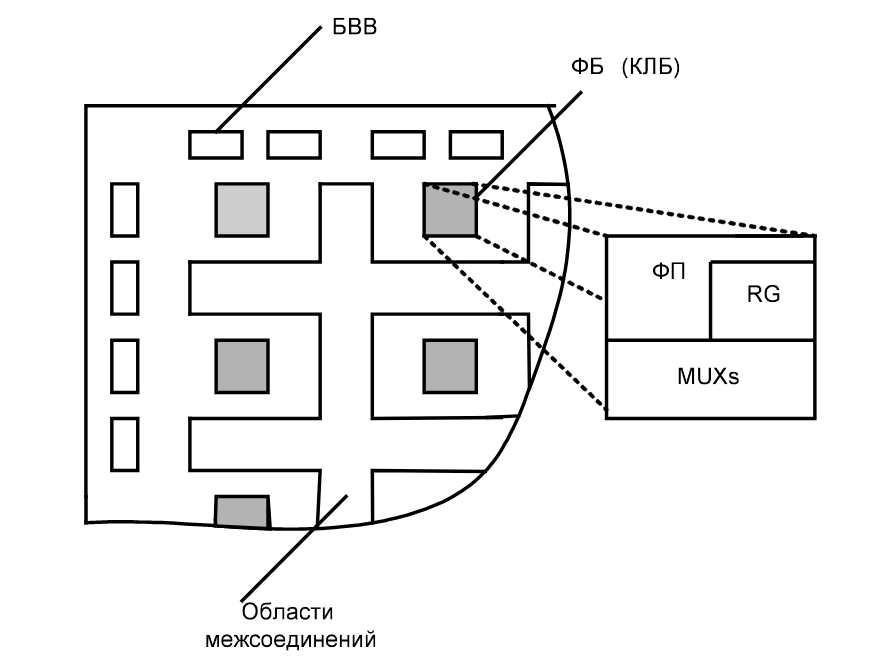
\includegraphics[scale=0.4]{ugrymov_fpga_artchitecture.png}
  \captionof{figure}{ Фрагмент базовой архитектуры FPGA \cite{ugrymov_digital_circuit_engineering} }
  \label{fig:domain:fpga:fpga_architecture}
\end{center}

Конфигурируемые логические блоки состоят из:
\begin{itemize}
  \item некоторого количества элементов выполняющих логические преобразования;
  \item набора мультиплексоров для перенаправления выходных сигналов логических преобразователей;
  \item триггеров для хранения значений сигналов.
\end{itemize}

Схема современного КЛБ на примере семейства Spartan компании \en{Xilinx} представлена на рисунке~\ref{fig:domain:fpga:clb}

\begin{center}
  \centering
  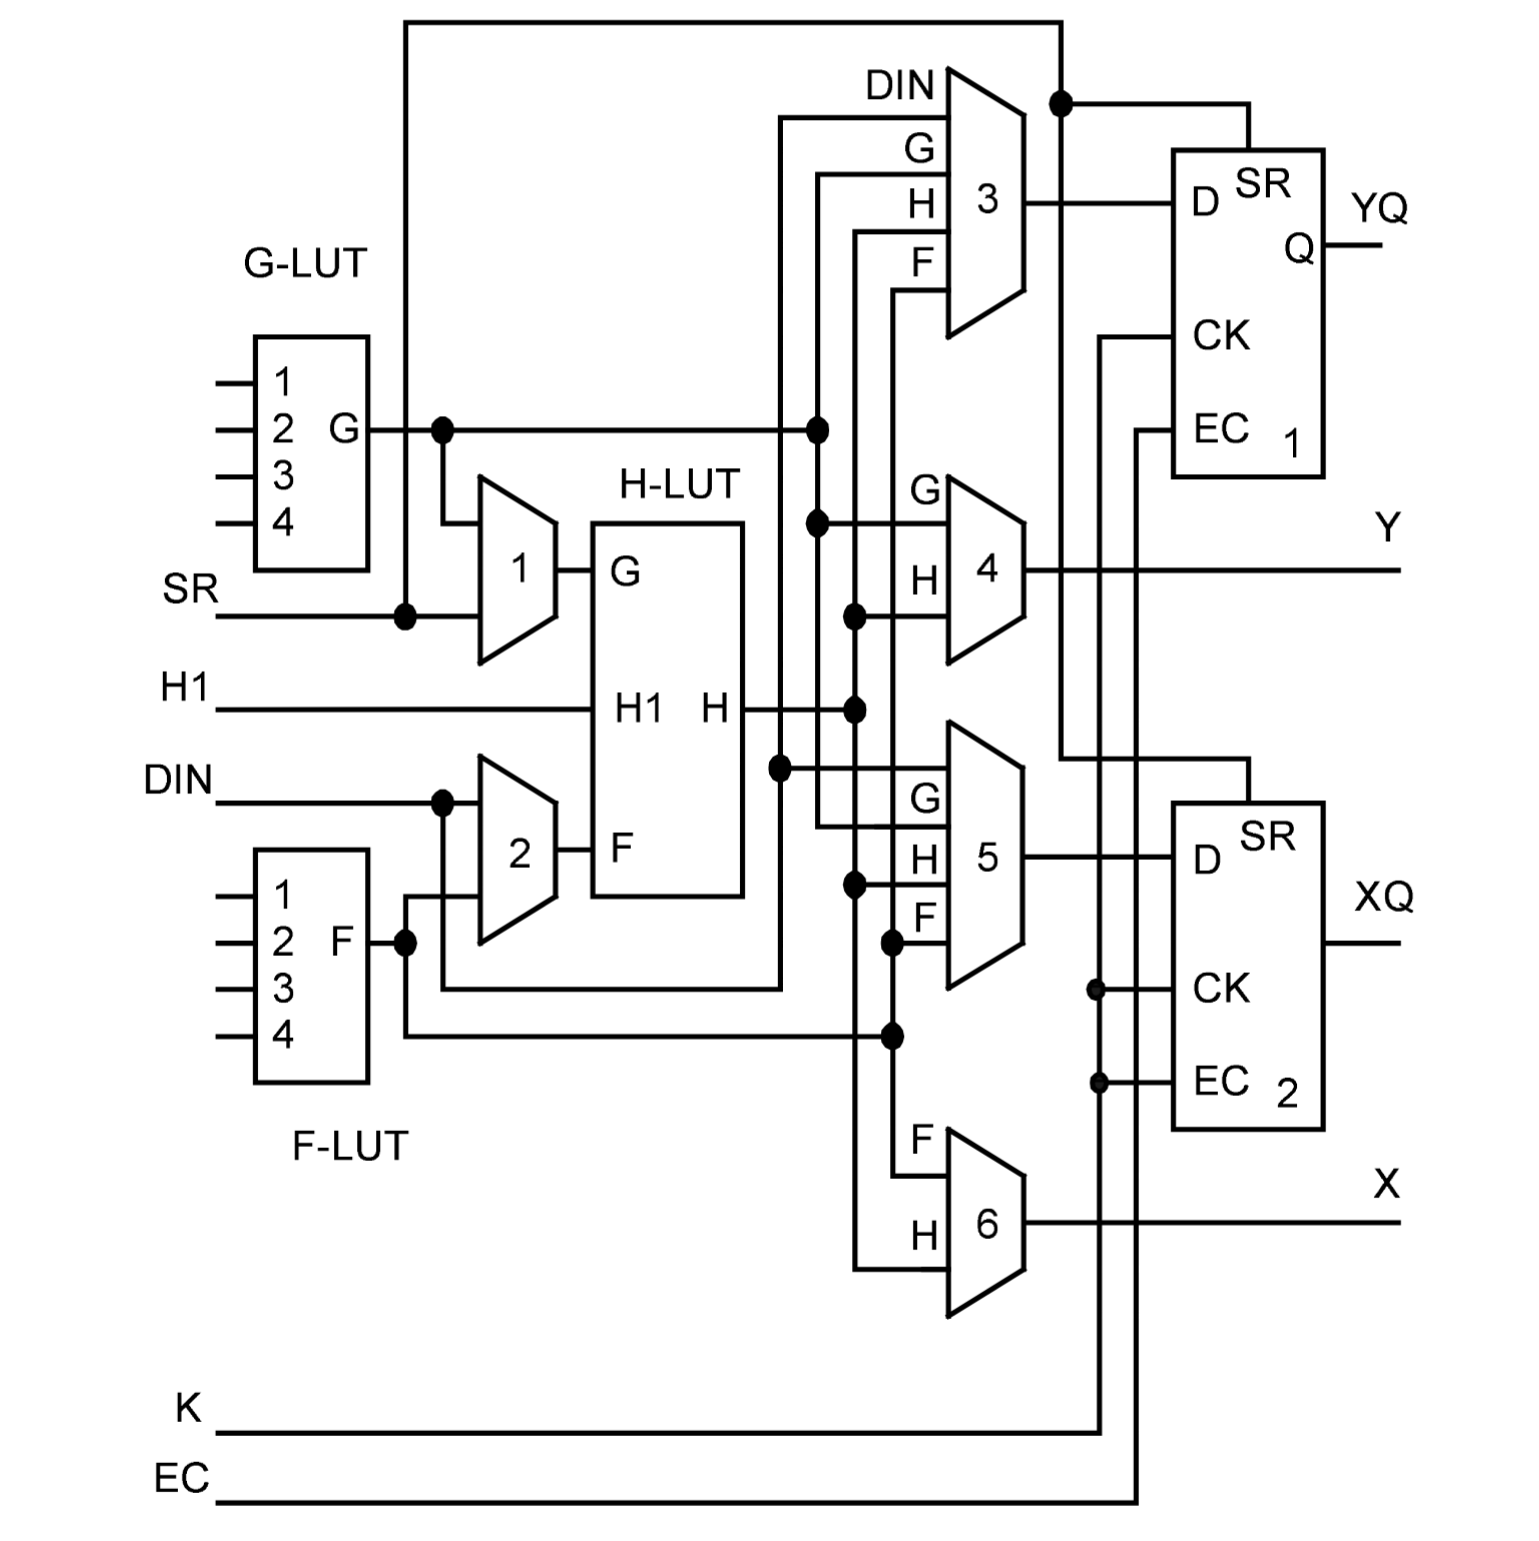
\includegraphics[scale=0.28]{ugrymov_fpga_clb.png}
  \captionof{figure}{ Логический блок семейства Spartan }
  \label{fig:domain:fpga:clb}
\end{center}

Системы межсоединений проектируются в широком диапазоне технологических и архитектурных решений.
Основная цель при построении эффективной системы коммутации --- обеспечение максимальной коммутируемости блоков
при минимальном количестве элементов связи с предсказуемыми задержками сигналов. Обозрение данной тематики задача достаточно нетривиальная,
стоит лишь отметить, что предсказуемость задержек это ключевой фактор в выборе микросхемы для проектирования системы реального времени.

С каждым выводом микросхемы ассоциируется свой блок ввода-вывода, который может настраиваться как вход, выход или двунаправленный вывод.
Упрощенная схема блока В/В представлена на рисунке~\ref{fig:domain:fpga:io}

\begin{center}
  \centering
  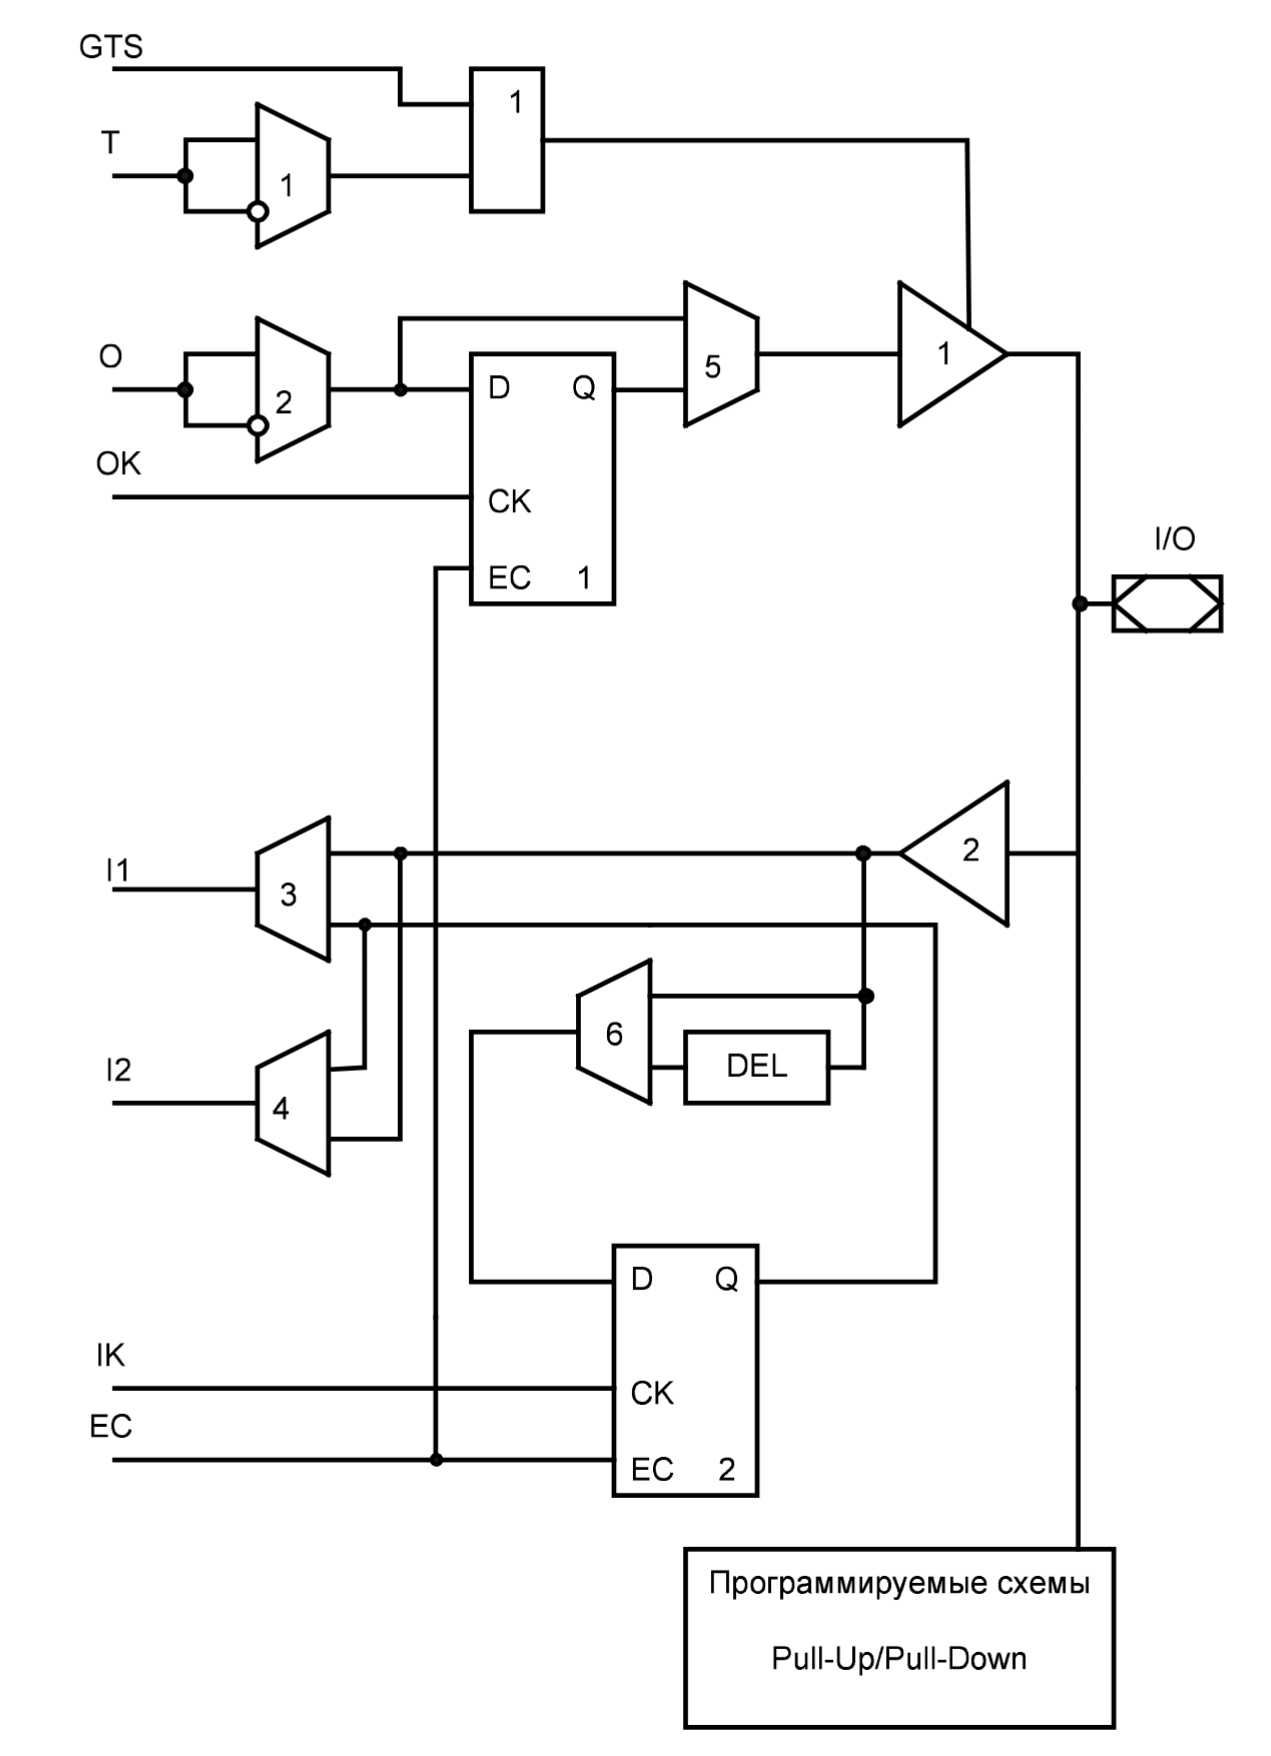
\includegraphics[scale=0.25]{ugrymov_fpga_io.png}
  \captionof{figure}{ Пример схемы блока ввода-вывода FPGA }
  \label{fig:domain:fpga:io}
\end{center}

Блок разделен на две части для работы как на вход, так и на выход. Основной интерес представляют буферы с тремя состояниями
1 и 2. Они имеют программируемые уровни сигналов(КМОП или ТТЛ), что заметно упрощает подключение пользовательских периферийных устройств
напрямую к микросхеме без подключения внешнего преобразователя уровня.

Основными игроками на рынке микросхем FPGA являются Xilinx и Altera. Они производят чипы применимые как в военной и космической сферах,
так и для потребительских нужд. Микросхемы широко варьируются по количеству логических блоков, размеру
статической памяти, количеству блоков ввода-вывода и поддержкой специфических блоков.

Однако для проектирования и отладки системы важен выбор не только микросхемы,
но и отладочной платы с необходимым набором периферии. Подробное сравнение отладочных
плат с микросхемами последнего поколения от различных производителей показывает, что
платы с микросхемами \en{Xilinx} наиболее разнообразны и представлены в более широком ценовом диапазоне,
чем платы Altera \cite{fpga_boards_comparison}.
Вследствие чего сделан выбор применения микросхем Xilinx в дипломном проекте.

\subsection{Сравнение cемейств микросхем Xilinx}
\label{sub:domain:fpga_comparison}

Компания Xilix является технологическим лидером на рынке производства микросхем FPGA.
На данный момент наиболее актуальная линейка микросхем --- Xilinx 7 series\cite{7_series_overview}.
Продукты данной линейки покрывают всевозможные требования к микросхеме: от низкого энергопотребления, малого размера, низкой цены до
поддержки высокоскоростных интерфейсов и большого количества логических и DSP (Digital Signal Processing) блоков.

Седьмое поколение микросхем Xilinx делится на 4 основные категории:
\begin{itemize}
  \item Spartan-7: для недорогих и маломощных систем, требующих высокую производительность ввода-вывода.
    Имеет наименьшую площадь посадочного места во всей линейке;
  \item Artix-7: оптимизирован для маломощных приложений с требованиями по высокой пропускной способности логических и DSP блоков.
    Обладает наиболее высоким параметром производительности на ватт;
  \item Kintex-7: микросхема с лучшим соотношением цены к производительности;
  \item Virtex-7: лучшая в классе производительность с применением новейших производственных технологий.
\end{itemize}

Так как в системах обработки видео с помощью FPGA блоки DSP выполняют роль сопроцессора, то
основная нагрузка ложится на саму микросхему. Исходя из этого следует подбирать микросхему
руководствуясь её предельной тактовой частоты и количества логических блоков\cite{7_series_selection_guide}.

Старшие микросхемы в линейке Spartan работают на частотах порядка 500 МГц, однако обладают слишком малым количеством
логических и DSP блоков.

FPGA линейки Virtex являются самым передовым решением компании, их характеристики превосходят необходимые требования,
но стоимость на порядок выше младших решений делает их выбор не оптимальным.

Семейства Kintex и Artix используют 28 нм техпроцесс, основное различие различается в количестве DSP блоков, что не является
ключевым фактором в выборе микросхемы. При схожих параметрах, микросхемы Artix стоят меньше чем Kintex\cite{artix_kintex_price_comparison},
что послужило основанием для выбора данного семейства в дипломном проекте.

% Плюсы fpga конкретно для DIP dark fantasies

% Параллелизм в алгоритмах обработки изображений существует в двух основых формах --- пространственный и временный.
% Реализации данных алгоритмов на FPGA потенциально могут использовать комбинацию двух форм.\cite{downton_dip_architectures}.

% В частости, в задачах обработки изображения, FPGA ценится за возможность применения в системах
% с динамической реконфигрурацией, в которых требуется быстрая смена настроек системы для подстраивания
% под изменяющиеся внешние параметры \cite{burns_fpga_run_time_reconf}.

% Можно добавить отдельную секцию про выбор платы, но это уже занадто

\subsection{Обзор платы AC701}
\label{sub:domain:ac701}

Плата AC701 от компании Xilinx представляет собой так называемый \en{evaluation board},
содержащую весь возможный набор периферийных устройств подключаемых к микропроцессору.
Среди них особый интерес представляют:
\begin{itemize}
  \item микросхема XC7A200T-2FBG676C семейства Artix-7;
  \item 1GB DDR3 SODIMM;
  \item программируемый осциллятор;
  \item FMC (FPGA Mezzanine Card);
  \item шина I2C разведённая ко всей программируемой на плате периферии;
  \item контроллер и коннектор HDMI.
\end{itemize}

Структурная схема платы представлена на рисунке~\ref{fig:domain:ac701:block_design}

\begin{center}
  \centering
  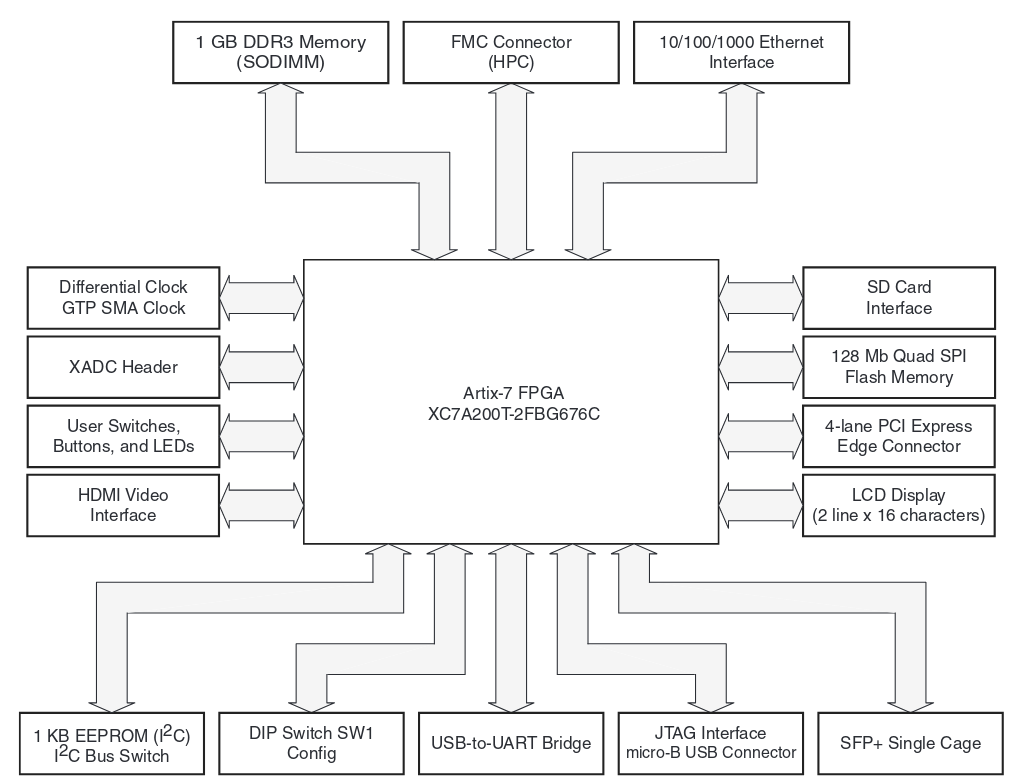
\includegraphics[scale=0.4]{ac701_block_design.png}
  \captionof{figure}{ Блок схема платы AC701 }
  \label{fig:domain:ac701:block_design}
\end{center}

Кадр HDTV видеопотока занимает порядка 1280 $\cdot$ 720 $\cdot$ 3 $=$ 2,76 МБ памяти. Размер SRAM памяти
микросхемы составляет 2,8 МБ, что позволяет буферизировать один кадр видеопотока. Однако большинство
алгоритмов обработки изображений работают со буфером памяти, в котором сохраняются промежуточные результаты
вычислений. Для таких целей объёма SRAM памяти становится недостаточно. Поэтому
для временного хранения потока приходящих кадров необходима динамическая память.   % Можно добавить ссылку на расчёты во введении или привести новые для 2160/1080

Программируемый осциллятор позволяет подключать к дополнительной периферии, например камере, тактовый сигнал произвольной частоты.
Для задания опорной частоты используется шина I2C. Частота варьируется от 10 МГц до 810 МГц. Высокие частоты достигаются применением дифференциальной пары.
Схема осциллятора представлена на рисунке~\ref{fig:domain:ac701:user_clock}

\begin{center}
  \centering
  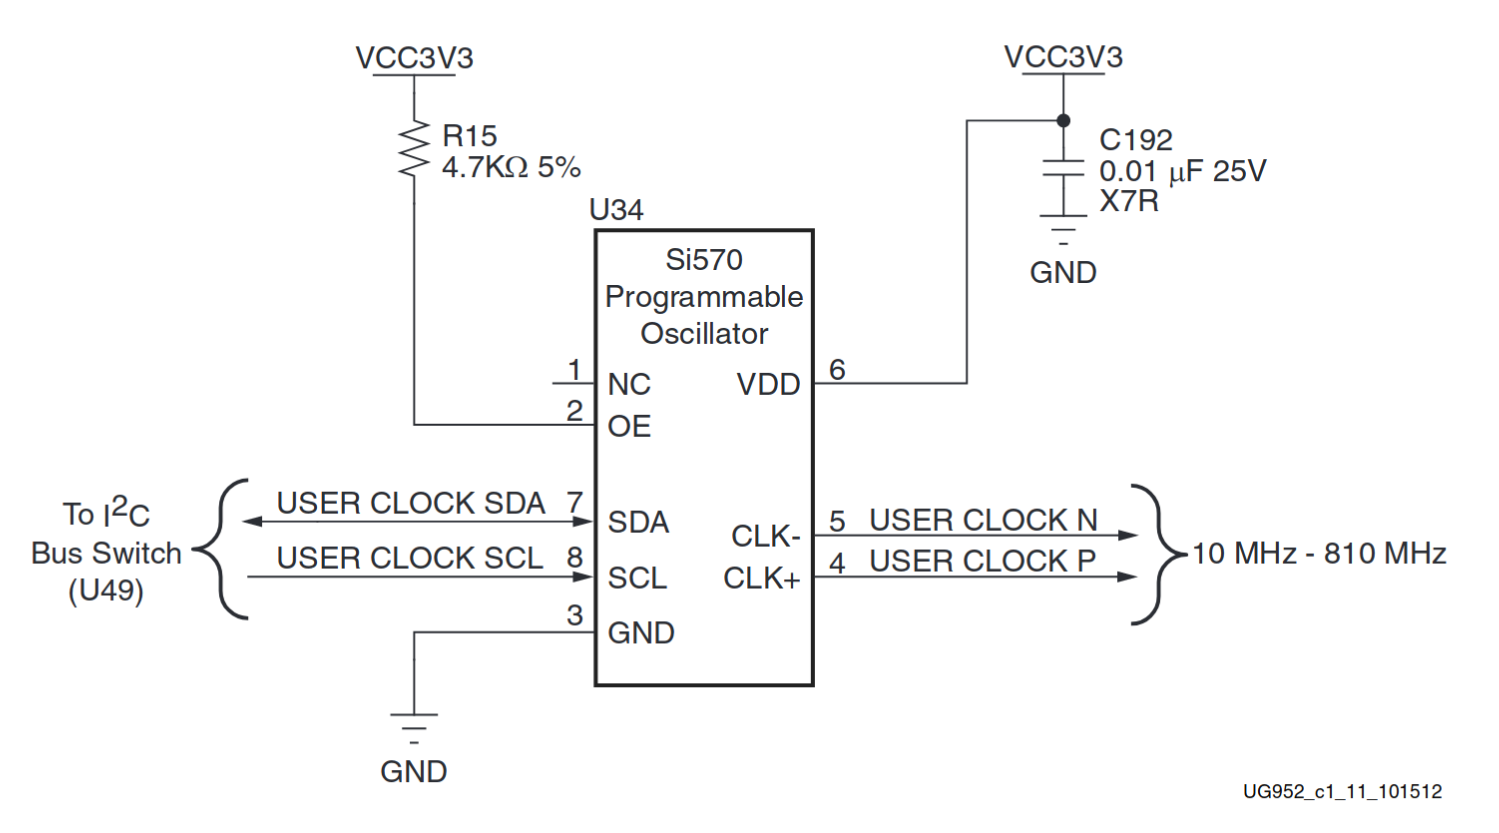
\includegraphics[scale=0.25]{ac701_user_clock.png}
  \captionof{figure}{ Программируемый осциллятор }
  \label{fig:domain:ac701:user_clock}
\end{center}

Подключение произвольных периферийных устройств осуществляется через разъём FMC, поддерживающий передачу
высокочастотных дифференциальный и однополярных сигналов на частотах до 9 ГГц\cite[c. 57]{ac701_user_guide}.
К таким устройствам относятся любые источники высокочастотных данных, такие как камеры, приёмники сигналов и так далее.

Программирование устройств на плате осуществляется посредством записи внутренних регистов по шине I2C. Она служит основным
инструментом настройки и диагностирования состояния компонентов на плате. Точный список устройств показан на
рисунке~\ref{fig:domain:ac701:i2c}

\begin{center}
  \centering
  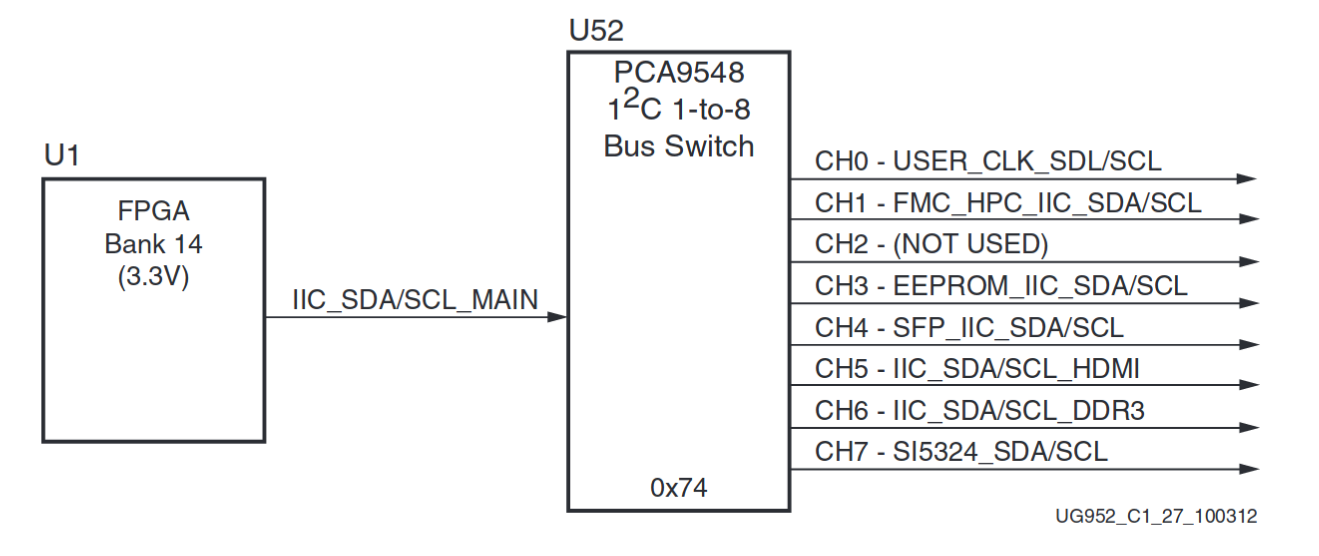
\includegraphics[scale=0.25]{ac701_i2c.png}
  \captionof{figure}{ Топология шины I2C }
  \label{fig:domain:ac701:i2c}
\end{center}

Обработанное видео передаётся через коннектор HDMI (\en{High Definition Multimedia Interface}) на устройство видеовывода либо дальнейшей обработки. В качестве
HDMI контроллера на плате установлен ADV7511KSTZ-P компании Analog Devices. Контроллер поддерживает передачу видео формата 1080p 60 Гц в
цветовом пространстве YCbCr 4:4:4, блоками по 24 бита.
Схема подключения контроллера представлена на рисунке~\ref{fig:domain:ac701:hdmi}

\begin{center}
  \centering
  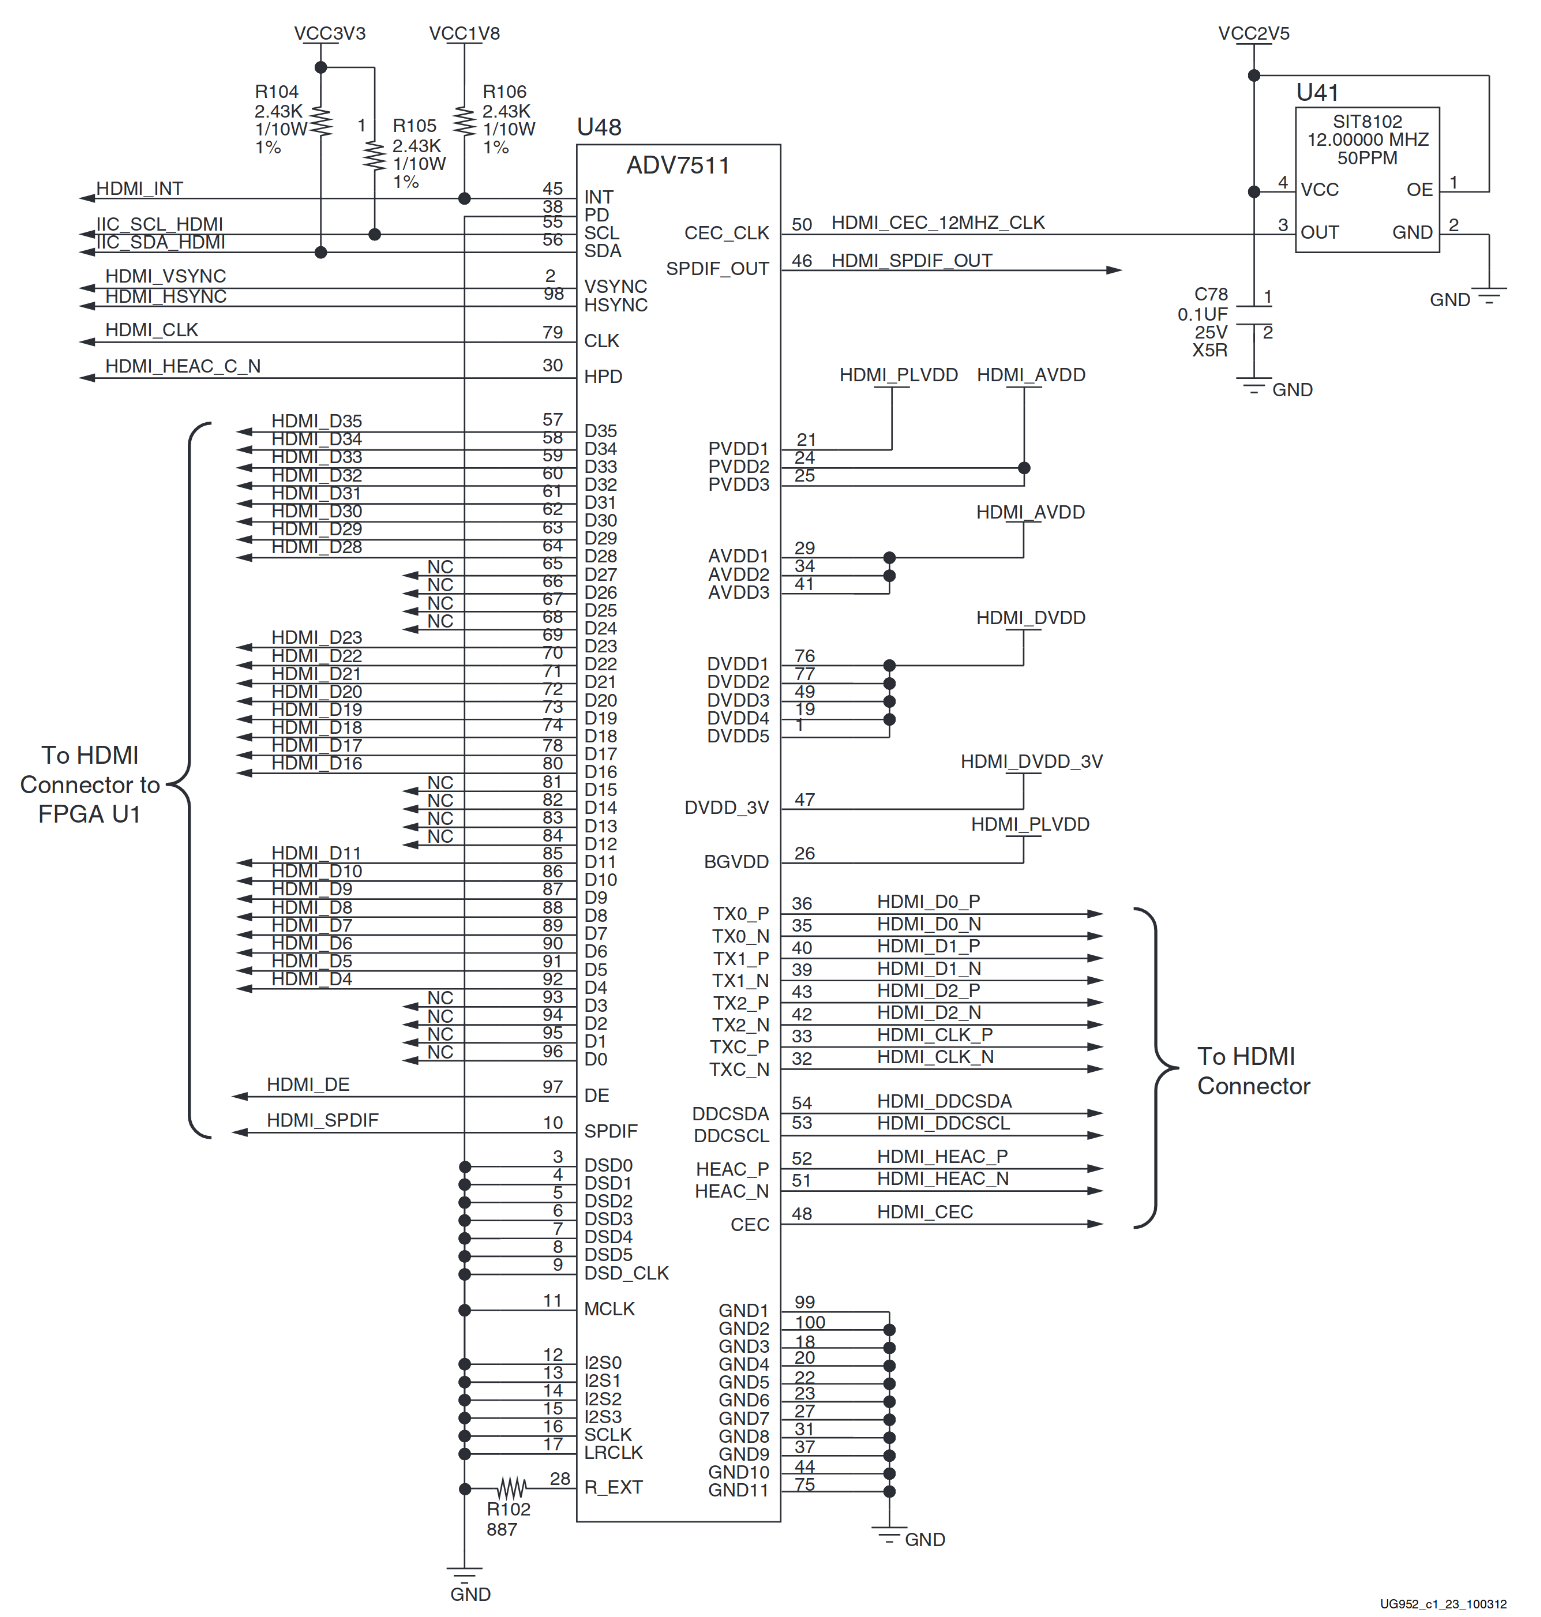
\includegraphics[scale=0.28]{ac701_hdmi.png}
  \captionof{figure}{ Схема подключения HDMI контроллера }
  \label{fig:domain:ac701:hdmi}
\end{center}

Более подробная информация о подключении, назначении внутренних регистров и режимах работы содержится в \cite{adv7511_datasheet}.

\subsection{Обзор камер}
\label{sub:domain:camera}

Одним из источников видео являются видеокамеры.

Оптические сенсоры современных камер производятся по двум технологиям: ПЗС и КМОП.
Основной принцип работы матрицы на приборе с зарядовой связью заключается в сдвиге заряда,
накопленного элементами ПЗС матрицы.
В свою очередь в КМОП-матрицах фоточувствительные элементы являются независимыми друг от друга единицами
и не влияют напрямую на накопленный друг другом заряд.
Несмотря на низкую светочувствительность КМОП-матриц по сравнению с ПЗС, их цена, энергопотребление и
быстродействие почти полностью вытеснили ПЗС-матрицы с рынка потребительской электроники, поэтому
в дальнейшем будут обозреваться КМОП-камеры.

Критерием выбора служит поддержка съёмки видео высокого разрешения (1280x720 HDTV и выше).
Большинство камер поддерживают либо меньшее разрешение, либо поставляются на платах с большим
количеством лишней периферии. Среди подходящих под требование наиболее выделяется модуль
MT9T031C12STCH ES компании Aptina. При разрешении 1280x720 частота кадров достигает 38 снимков в секунду,
что приемлемо для восприятия человеком. Так как современные FPGA работают от напряжения 3.3 В, данная камера
может питаться напрямую от источника питания для платы без преобразований\cite{image_sensor_datasheet}.
Схема подключения камеры представлена на рисунке~\ref{fig:domain:camera:camera_configuration}

\begin{center}
  \centering
  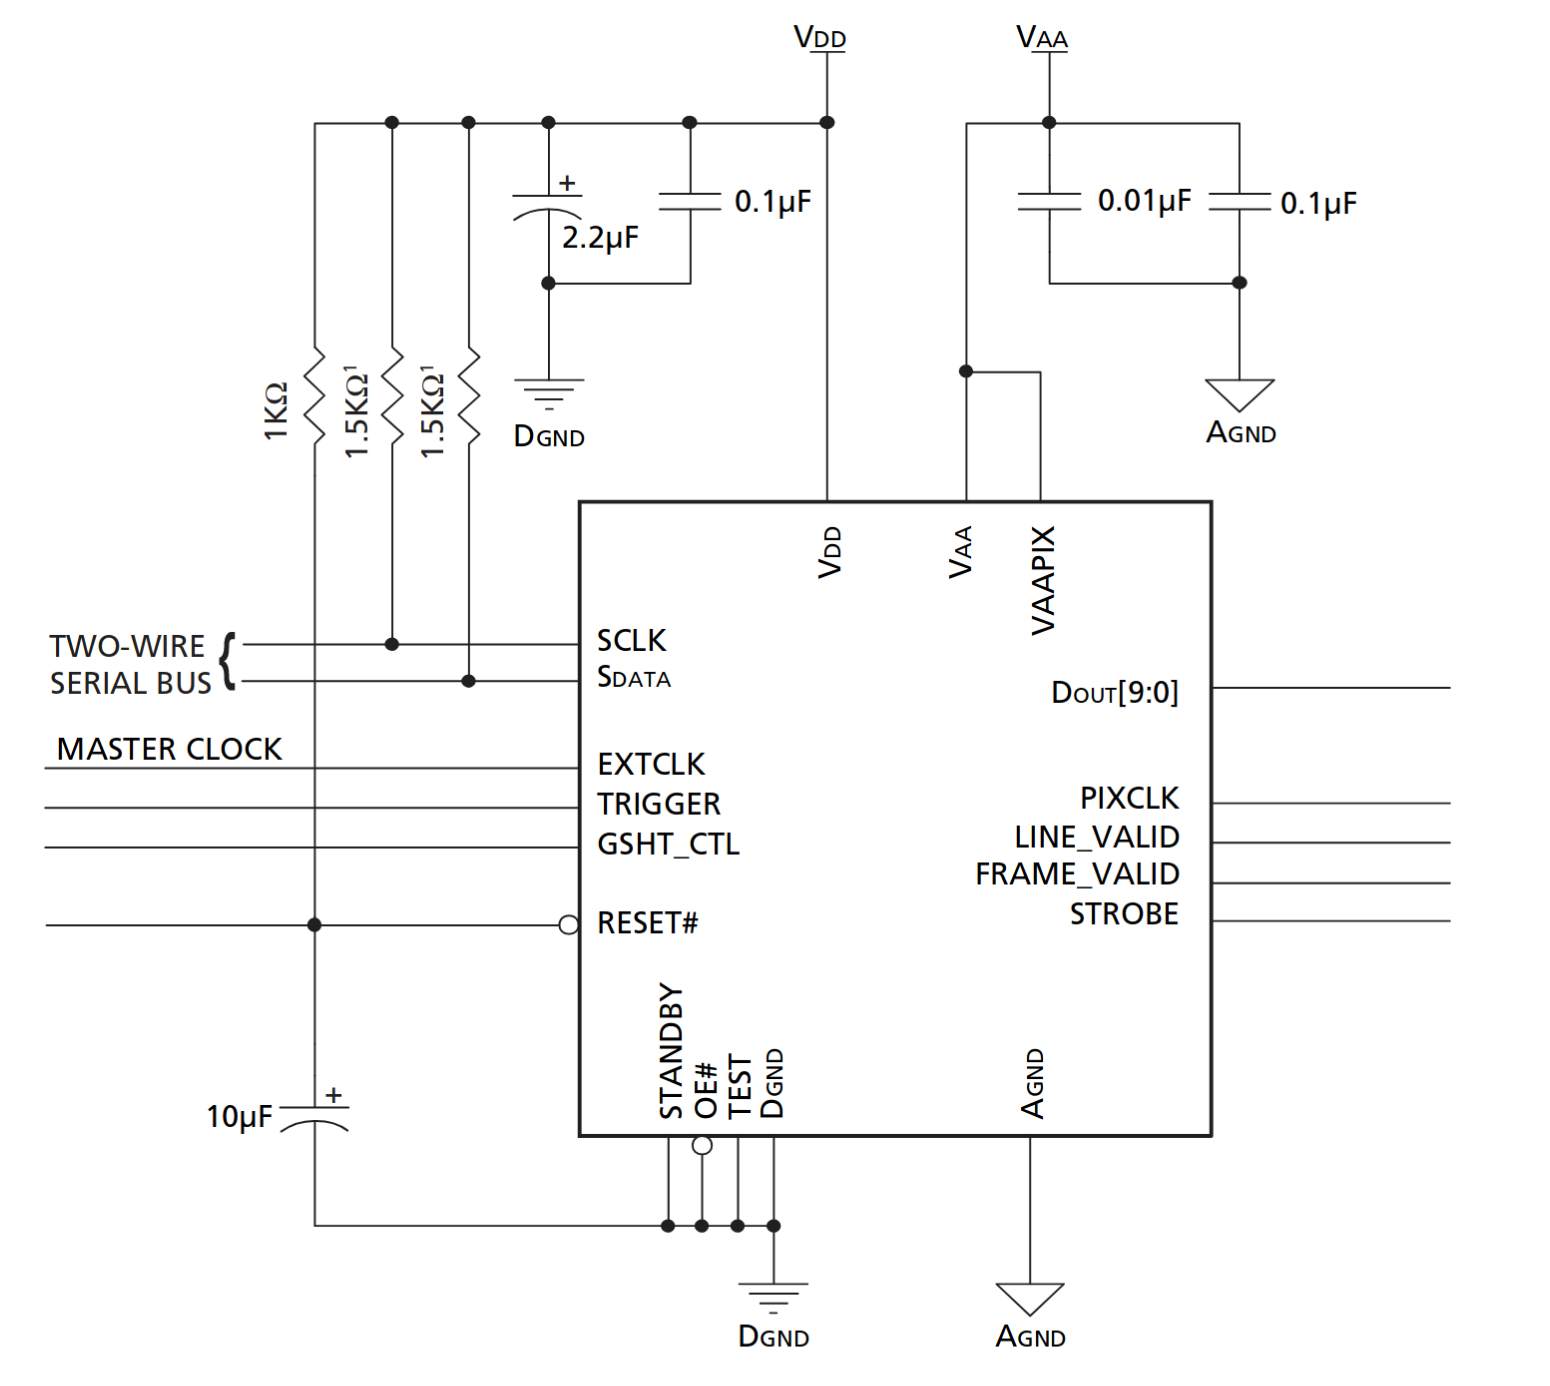
\includegraphics[scale=0.22]{camera_configuration.png}
  \captionof{figure}{ Схема подключения камеры \cite{camera_module_datasheet} }
  \label{fig:domain:camera:camera_configuration}
\end{center}

% Это чтобы не ехали подписи
В качестве синхросигналов используется HSYNC и VSYNC, видеоданные передаются по 10-битной параллельной шине.
Модуль поддерживает различные режимы работы, одним из которых является режим пропуска областей кадра, для
уменьшения объёма передаваемых данных. Настройка камеры производится записью внутренних регистров по протоколу I2C.
% \subsection{Microblaze}
% \label{sub:domain:microblaze}

\subsection{Обзор аналогов}
\label{sub:domain:alternatives}

Системы обработки видео на FPGA получили распространение в конце 1990-ых годов, когда
производство программируемой логики стало коммерчески выгодным. Работы делятся на несколько
направлений: портирование алгоритмов ЦОС с последующими замерами времени выполнения,
проектирование систем реального времени, создание систем обработки видео для встраиваемых систем.

Данные системы, как правило, не обладают модульной архитектурой: попытка внесения изменений,
например, добавление нового фильтра в цепочку обработки, требует изменения большей части
составных блоков.
К примеру, в работе \cite{meng_fpga_based_video_processing} разработанная система
имеет линейную архитектуру, не предполагая наличия управляющей логики, что существенно сужает круг
её применения. Архитектура линейной системы представлена на рисунке~\ref{fig:domain:alternatives:linear_architecture}

\begin{center}
  \centering
  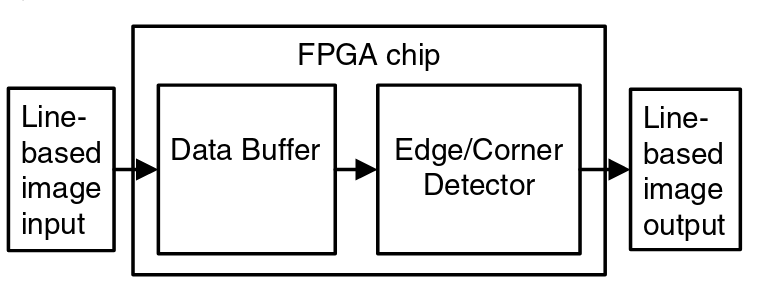
\includegraphics[scale=0.28]{system_linear_architecture.png}
  \captionof{figure}{ Архитектура линейной системы обработки видео }
  \label{fig:domain:alternatives:linear_architecture}
\end{center}

Другие системы \cite{embeded_real_time_fpga_modular} разделяют управляющую
и обрабатывающую логику, однако не поддерживают добавления блоков обработки в произвольное
место в потоке данных(перед конвертацией видео во внутренний формат FPGA или после).
Схема данной системы представлена на рисунке~\ref{fig:domain:alternatives:microblaze_architecture}

\begin{center}
  \centering
  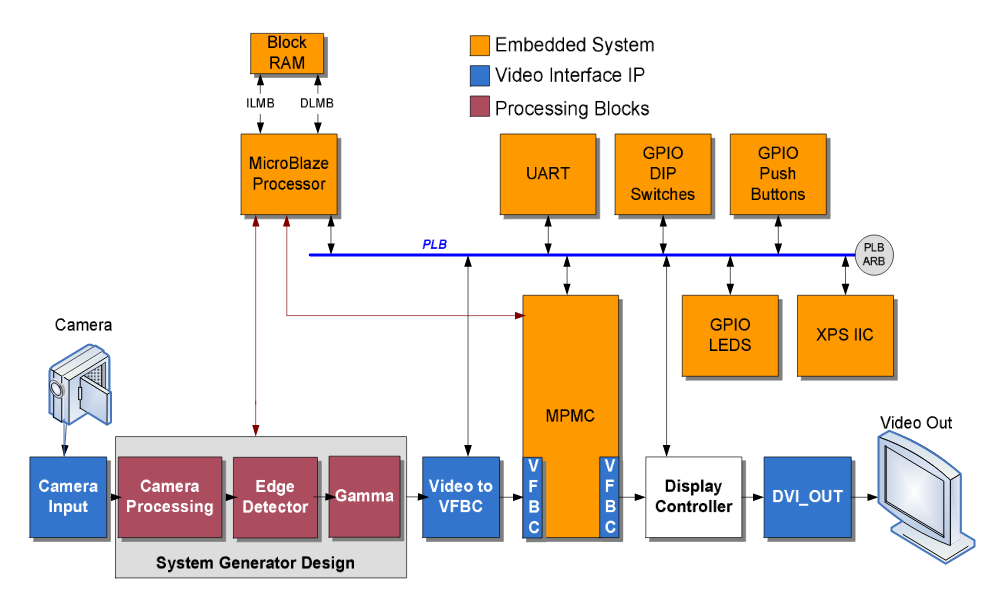
\includegraphics[scale=0.3]{system_microblaze_architecture.png}
  \captionof{figure}{ Потоковая система обработки видео }
  \label{fig:domain:alternatives:microblaze_architecture}
\end{center}

Наиболее удачным решением является комбинация линейной системы, поддерживающей интеграцию сторонних модулей в цепь обработки, и
выделенного модуля управления, для настройки и отслеживания состояния системы.


\section{СТРУКТУРНОЕ ПРОЕКТИРОВАНИЕ}
\label{sec:structural}

После проработки теоретических вопросов связанных с разработкой системы и
составления списка необходимых требований к системе, необходимо разбить проектируемую систему
на функциональные блоки. Данный подход обеспечивает архитектурную гибкость, позволяя
модифицировать или заменять функциональные блоки без изменения системы в целом.

В разрабатываемой системе обработки видео можно выделить следующие блоки:

\begin{itemize}
  \item блок камеры;
  \item блок Video DMA для входного видеопотока;
  \item блок ОЗУ;
  \item блок Video DMA для выходного видеопотока;
  \item блок микропроцессора;
  \item блок контроллера HDMI;
  \item блок контроллера I2C.
\end{itemize}

Структурная схема, иллюстрирующая перечисленные блоки и связи
между ними приведена на чертеже ГУИР.400201.064 Э1.

Каждый функциональный блок выполняет свой круг задач и взаимодействует с другими блоками
посредством различных аппаратных интерфейсов и протоколов шины.

Рассмотрим более подробно функциональные блоки системы.

\subsection{Блок камеры}
\label{sec:structural:camera}

Блок камеры является инициатором входного видеопотока. Перед началом работы происходит
процесс инициализации, где задаётся разрешение видео, количество кадров в секунду,
различные режимы выборки и т.д. Видеопоток формируется в формате Bayer RGB, в котором
на каждый итоговый пиксель приходится 25\% красных, 25\% синих и 50\% зеленых элементов.
Такая конфигурация светофильтра даёт большую разрешающую способность в зелёной области спектра,
что соответствует особенностям человеческого зрения. Сформированный поток пикселей интерполируется
контроллером камеры, после чего при помощи внешней синхронизации передаётся на преобразователь
RGB в протокол AXI4-Stream(далее AXIS). Модули по обработке видео могут встраиваться в систему как до преобразования в
AXIS, так и на последующих этапах.

% Дописать ещё чё нить

\subsection{Блок Video DMA для входного видеопотока}
\label{sec:structural:vdma_in}
Блок Video DMA(далее VDMA) для входного видеопотока обеспечивает высокоскоростной прямой доступ к памяти
между ОЗУ и видеопериферией по протоколам AXI4 и AXIS. Master-устройством выступает контроллер ОЗУ,
инициируя транзакцию по передаче части кадра из Slave-устройства преобразователя в блок памяти ОЗУ.
Такое решение позволяет исключить микропроцессор из потока обработки данных, где он является
критическим местом по производительности. VDMA поддерживает режим пакетного обмена, дополнительно
ускоряя обмен между камерой и ОЗУ.


\section{ФУНКЦИОНАЛЬНОЕ ПРОЕКТИРОВАНИЕ}
\label{sec:functional}

В данном разделе рассматривается проектирование системы на функциональном уровне, в
соответствии с полученной ранее структурной схемой. Для обеспечения модульности,
на данном уровне используются IP-ядра и стандартизированные протоколы обмена данными
между ними.

Разработка устройств на FPGA заметно облегчается механизмом IP-ядер (\en{Intellectual Property}) --- готовых
блоков для проектирования микросхем и прочих цифровых устройств. IP-ядра представляют собой
конфигурируемый блок цифрового устройства, описанный на HDL (\en{Hardware Description Language}).
Как правило, разработчик IP-ядра включает в него широкий перечень изменяемых параметров,
позволяя сторонним разработчикам переиспользовать ядро в своих целях, внося минимум необходимых
изменений вручную.

\subsection{Структура системы}
\label{sec:functional:structure}

Разрабатываемая система разделена на несколько блоков:

\begin{itemize}
  \item Video In to AXI4-Stream --- блок преобразования видеопотока в \en{AXI4-Stream};
  \item VDMA In --- Video DMA для входного видеопотока;
  \item Memory Interface Generator --- контроллер DDR-пямяти;
  \item VDMA Out --- Video DMA для выходного видеопотока;
  \item AXI CLKGEN --- генератор тактового сигнала для контроллера \en{HDMI};
  \item AXI HDMI TX --- блок управления контроллером \en{HDMI};
  \item AXI Camera I2C --- блок управления камерой посредством I2C;
  \item AXI HDMI I2C --- блок конфигурации контроллера \en{HDMI} посредством \en{I2C};
  \item AXI UART-Lite --- блок контроллера \en{UART};
  \item Microblaze --- soft-core микропроцессор для управления работой блоков;
  \item Microblaze Debug Module --- отладочный модуль для \en{Microblaze};
  \item Microblaze Local Memory --- локальная память \en{Microblaze};
  \item Processor System Reset --- контроллер сброса системы.
    % Докинуть сюда контроллер прерываний
\end{itemize}

Чертёж системы приведён ГУИР.400201.064 Э2.

\subsection{Video In to AXI4-Stream}
\label{sec:functional:video_in_to_axi4stream}
Большинство IP-ядер нацеленные на обработку видео используют протокол AXI4-Stream для
обмена данных. Передача видео между системами, обычно, сопровождается сигналами гашения и
синхросигналами для указания вертикальной и горизонтальной синхронизации, а также
валидности данных в видеопотоке. Интерфейс DVI (Digital Visual Interface) является
одним из представителей такого режима передачи. Ядро Video In to AXI4-Stream преобразует
входящий видеопоток и его управляющие и синхросигналы в протокол AXI4-Stream для
связи с другими блоками, поддерживающими данный протокол. На вход блоку поступает
видеопоток в параллельном виде, частота прорисовки одного пикселя и следующий набор
тайминговых сигналов:

\begin{itemize}
  \item Vsync, Hsync, Data Valid;
  \item Vblank, Hblank, Data Valid;
  \item Vsync, Hsync, Vblank, Hblank, Data Valid.
\end{itemize}

Для полноценной работы блока достаточно любого из этих трёх наборов сигналов. Выбор конкретного
множества существеннен при исползовании детектора Video Timing Controller.
Внутреннее устройство блока представлено на рисунке~\ref{fig:functional:vid_in_to_axi4stream:inner_structure}

\begin{center}
  \centering
  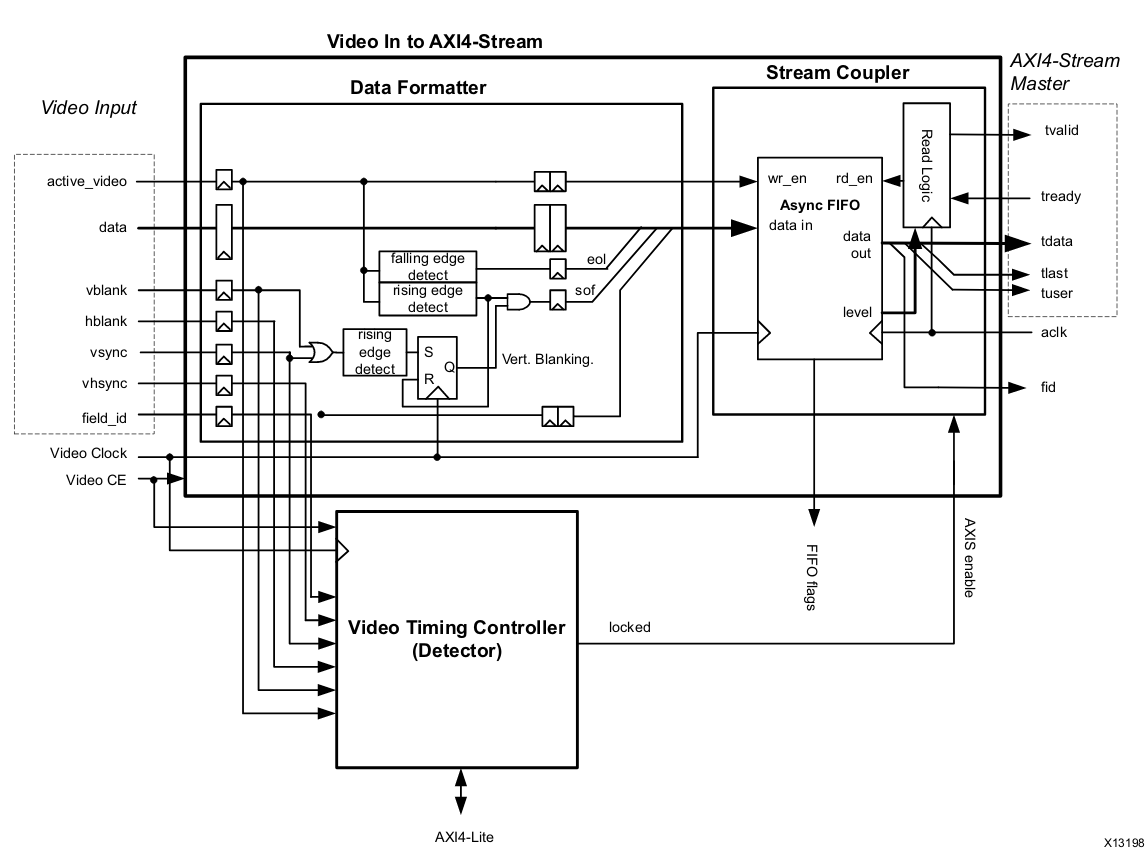
\includegraphics[scale=0.4]{vid_in_to_axi4stream.png}
  \captionof{figure}{ Структурная схема ядра Video In to AXI4-Stream }
  \label{fig:functional:vid_in_to_axi4stream:inner_structure}
\end{center}

Описание сигналов общего назначения:

\begin{itemize}
  \item ACLK --- тактовый сигнал шины AXI4-Stream, входной видеосигнал сэмплируется по фронту
    тактового импульса, выходной сигнал \en{AXI4-Stream} изменяется через некоторое время после фронта ACLK;
  \item ACLKE --- разрешение тактирования, активный высокий уровень. В случае подачи низкого уровня
    приостанавливает работу выходной шины, сохраняя внутреннее состояние блока. При переходе
    из низкого уровня в высокий входной видеопоток не сэмплируется, таким образом подавляя перезаписывание
    кадра в памяти блока.
  \item VCE (Video Clock Enable) --- разрешение работы внутренних регистов, отвечающих за работу с видео.
    Используется, когда видеосигнал подаётся с большей частотой, чем подразумевает стандарт синхронизации видео.
\end{itemize}

Описание видеосигналов приведено в таблице~\ref{table:functional:vid_in_to_axi4stream:video_signals}

\begin{table}[ht]
  \caption{Описание видеосигналов блока Video In to AXI4-Stream}
  \label{table:functional:vid_in_to_axi4stream:video_signals}
  \begin{tabular}{| >{\centering}m{0.18\textwidth}
                  | >{\centering}m{0.17\textwidth}
                  | >{\centering\arraybackslash}m{0.57\textwidth}|}
   \hline
    Обозначение сигнала & Разрядность & Краткое описание \\
    \hline
    ACTIVE & 1 & Валидность видеоданных. 1 --- активный видеопоток,
                        0 --- отсутствие видеоданных \\
    \hline
    DATA & 10 & Параллельный видеопоток \\
    \hline
    HBLNK & 1 & Строчный гасящий импульс, активный высокий уровень \\
    \hline
    HSYNC & 1 & Сигнал горизонтальной синхронизации, активный высокий уровень \\
    \hline
    VBLNK & 1 & Кадровый гасящий импульс, активный высокий уровень \\
    \hline
    VSYNC & 1 & Сигнал вертикальной синхронизации, активный высокий уровень \\
    \hline
  \end{tabular}
\end{table}

Описание сконвертированного видеопотока приведено в таблице~\ref{table:functional:vid_in_to_axi4stream:output_signals}

\begin{table}[ht]
  \caption{Описание выходных сигналов блока Video In to AXI4-Stream}
  \label{table:functional:vid_in_to_axi4stream:output_signals}
  \begin{tabular}{| >{\centering}m{0.18\textwidth}
                  | >{\centering}m{0.17\textwidth}
                  | >{\centering\arraybackslash}m{0.57\textwidth}|}
    \hline
    Обозначение сигнала & Разрядность & Краткое описание \\
    \hline
    TDAT & 32 & Видеоданные, соответствует AXI4-Stream TDATA \\
    \hline
    TVAL & 1 & Валидность видеоданных, соотвествует AXI4-Stream TVALID \\
    \hline
    TRDY & 1 & Готовность Slave-устройства принять данные, соотвествует AXI4-Stream TREADY \\
    \hline
    TLAST & 1 & Сигнал End of Line, соотвествует AXI4-Stream TLAST \\
    \hline
    TUSER & 1 & Начало нового кадра, соотвествует AXI4-Stream TREADY \\
    \hline
  \end{tabular}
\end{table}

По спецификации AXI4-Stream разрядность линий TDATA должна быть кратна 8-ю битам. % Вот тут хер пойми как правильно просклонять
Если входной видеопоток не кратен 8 битам, то данные должны быть дополнены нулями
начиная с старшего значащего бита. Таким же образом упакован выходной видеопоток.
На рисунке~\ref{fig:functional:vid_in_to_axi4stream:packed_output} показан
видеопоток с 12-ю битами на один канал формата RGB.

\begin{center}
  \centering
  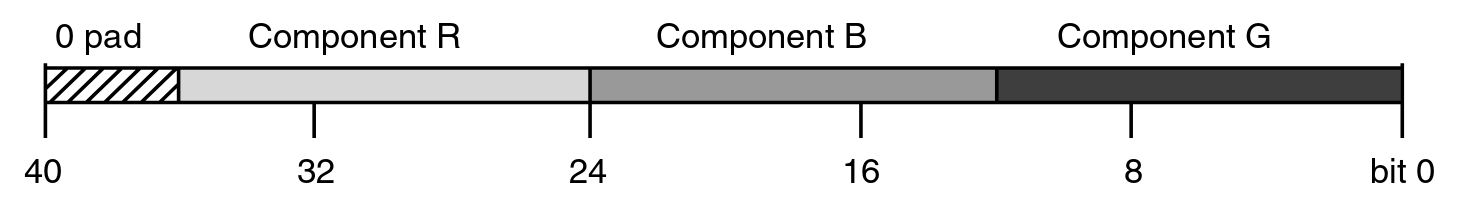
\includegraphics[scale=0.3]{vid_in_to_axi4stream_output.png}
  \captionof{figure}{ Упаковка выходного видеопотока в формате RGB }
  \label{fig:functional:vid_in_to_axi4stream:packed_output}
\end{center}

На входы блока подаётся видеопоток с CMOS-камеры. Для этого ядро конфиругируется в режим
\en{Image Sensor}, выбирается нужная разрядность (в данном случае 10 бит). Так как различные
матрицы выдают цветовые каналы в различном порядке, необходимо сконфигурировать порядок цветовых
каналов во входном видеопотоке.

При подключении камеры линии отрисовки пикселей, вертикальной и горизонтальной синхронизации,
валидности данных подключаются напрямую к контроллеру камеры, на линии VCE и ACLKE подаётся высокий уровень,
линия ACLK к общей линии тактирования системы. Для подачи выского или низкого уровня используется
специальный блок констант.

% Что нибудь ещё про камеру сказануть

\subsection{VDMA In}
\label{sec:functional:vdma_in}
Для обработки изменений в частоте кадров или изменения их размеров в приложениях
связанных с видеоконтентом используют кадровые буферы. Скоростной обмен между
таким буфером и системой обработки необходим: основные временные затраты
приходятся на передачу блоков данных из буфера и запись в него модифицированных частей кадра.

Ядро VDMA предоставляет возможность для высокоскоростного обмена между \en{AXI4-Stream} видеоинтерфейсом
и стандартным \en{AXI4}, разгружая управляющее устройство от активного контроля передачи.

Блок работает как стандартное устройство DMA, путём записи в регистры размера передаваемого блока данных,
начального адреса записи или чтения и количества циклов повторения операции. Оптимизация подобных
операций на микропроцессоре крайне затруднительна.

Блок VDMA оптимизирован для работы с непрерывным потоком данных, благодаря пакетному режиму передачи.
VDMA, в отличие от AXI DMA, имеет дополнительные линии для поддержки передачи видео без потери
сигналов развёртки и частоты отрисовки пикселей, что в дальнейшем можно использовать для смены частоты кадров.

%Добавить текст, чтобы всё съехало на новый лист
Внутреннее устройство блока представлено на рисунке~\ref{fig:functional:vdma_in:inner_structure}

\begin{center}
  \centering
  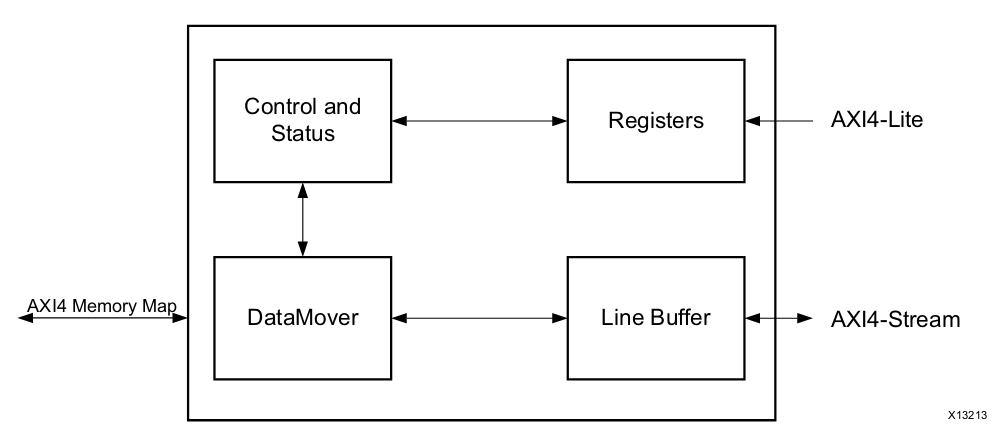
\includegraphics[scale=0.4]{vdma_structure.png}
  \captionof{figure}{ Структурная схема ядра VDMA }
  \label{fig:functional:vdma_in:inner_structure}
\end{center}

После программирования регистров по шине AXI4-Lite, блок управления и статуса генерирует список команд
для блока \en{DataMover}, чтобы инициировать команды чтения и записи интерфейса \en{AXI4 master}.
Асинхронный строковый буфер используется как временное хранилище пикселей с целью их последующей
записи на интерфейс \en{AXI4-Memory Map} или AXI4-Stream.

В случае записи VDMA прингимает кадры по slave интерфейсу AXI4-Stream и записиывает
их в память системы по master интерфейсу AXI4 master. В случае чтения ядро считывает
кадры по master интерфейсу AXI4 из системной памяти и перенаправляет их на master интерфейс
AXI4-Stream. Чтение и запись происходят независимо. Блок поддерживает возможность синхронизировать
входящие или исходящие кадры с внешним тактовым сигналом.

Основные возможности:
\begin{itemize}
  \item совместимость с протоколом AXI4 позволяет использовать модуль в любых приложениях, не разрабатывая
    собственный протокол высокоскоростной передачи данных;
  \item ядро поддеживает разрядность шины AXI4 в 32, 64, 128, 256, 512 и 1024 бита;
  \item ядро поддеживает разрядность шины AXI4-Stream по множителям 8 до 1024 бит;
  \item встроенные 32 кадровых буфера для 32-битного адресного пространства;
  \item опционально используется контроллер автоматического выравниваения обращений к памяти,
    транслируя обращение к произвольному адресу в выровненное. Поддерживается вплоть до 64-битной
    шины \en{AXI4-Stream};
  \item каждый канал VDMA может быть синхронизирован с другим при помощи \en{Genclock}, не позволяя
    при этом обоим каналам обращаться к одному и тому же кадровому буферу;
  \item поддержка асинхронных синхросигналов для различных типов AXI интерфейсов;
  \item блок способен динамически изменять частоту тактирования AXI4-Stream интерфейса,
    что позволяет передавать кадры с частотой и разрешением, отличным от исходных;
  \item поддержка различных механизмов синхронизации кадров, используя пользовательские линии
    шин AXI4.
\end{itemize}

Описание входных сигналов общего назначения приведено в таблице~\ref{table:functional:vmda_in:common_signals}

\begin{table}[ht]
  \caption{Описание входных сигналов общего назначения блока VDMA}
  \label{table:functional:vmda_in:common_signals}
  \begin{tabular}{| >{\centering}m{0.18\textwidth}
                  | >{\centering}m{0.17\textwidth}
                  | >{\centering\arraybackslash}m{0.57\textwidth}|}
   \hline
    Обозначение сигнала & Разрядность & Краткое описание \\
    \hline
    SC & 1 & тактовый сигнал AXI4-Lite \\
    \hline
    S2MC & 1 & тактовый сигнал AXI4-Stream to Memory Map \\
    \hline
    SS2MC & 1 & тактовый сигнал slave AXI4-Stream to Memory Map \\
    \hline
    ARST & 1 & сигнал сброса AXI4-Lite \\
    \hline
    ACLK & 1 & тактовый сигнал шины AXI4-Lite \\
    \hline
  \end{tabular}
\end{table}

Рассмотрим сигналы, используемые во входном VDMA при считывании кадров с преобразователя и последующей их передаче
в оперативную память. Для этого применяется 3 AXI интерфейса: AXI4-Lite для конфигурации ядра,
slave интерфейс AXI4-Stream to Memory Map для считывания входящего видеопотока и master интерфейc AXI4
для записи потока в оперативную память.

\section{РАЗРАБОТКА ПРОГРАММНЫХ МОДУЛЕЙ}
\label{sec:software_modules}

После проектирования аппаратной базы системы обработки видеопотока
необходимо разработать программный слой проекта. Конфигурация системы
осуществляется при помощи микропроцессора MicroBlaze. Она делится
на два множества: конфигурирование IP-блоков по протоколу AXI4-Lite и
внешней периферии, такой как контроллер HDMI и CMOS-камера, посредством
шины I2C. Рассмотрим подробнее часть функций.


Так как работа с контроллером HDMI происходит по протоколу I2C, то
сперва необходимо задать адрес устройства контроллера на этой шине.
Для этого необходимо проинициализировать блок AXI HDMI TX адресом контроллера,
взаимодействие с блоком происходит по шине AXI4-Lite.
Для этого вызывается библиотечная функция \texttt{HAL\_paltform\_init}, которая
задаёт адрес на шине I2C и адрес устройства сброса.

Для поддержки произвольного адреса контроллера на шине используется макроподстановка,
результат которой зависит от того, объявлен ли произвольный адрес контроллера в файле
BSP (\en{Board Support Package}):
\medskip
\begin{lstlisting}[style=C]
#ifdef XPAR_AXI_IIC_0_BASEADDR
	HAL_platform_init(XPAR_AXI_IIC_0_BASEADDR, XPAR_AXI_PSR_0_BASEADDR);
#else
  	HAL_platform_init(XPAR_AXI_IIC_MAIN_BASEADDR, XPAR_AXI_PSR_0_BASEADDR);
#endif
\end{lstlisting}
\medskip

После инициализации адреса контроллера необходимо рассчитать параметры
частоты для блока AXI CLKGEN, который тактирует контроллер HDMI.
Частота генериуемого тактового сигнала задаётся путём записи нужных
значений в регистры блока управления тактовыми сигналами. Рассмотрим
примитивы по работе с MMCM.

Первым примитивом, необходимым для отслеживания состояния блока, является
чтение из блока управления тактовыми сигналами. Так как работа с блоком происходит
не напрямую, а через аппаратную прослойку, то чтение ргеистров происходит со смещением
от адреса блока CLKGEN:
\medskip
\begin{lstlisting}[style=C]
  static void read(unsigned long register, unsigned long *value)
  {
	*value = Xil_In32(CF_CLKGEN_BASEADDR + register);
  }
\end{lstlisting}
\medskip

Чтение производится по шине AXI4-Lite, а так как микропроцессор реализует
отображение периферийных устройств в память, то чтение представляет собой не что иное,
как разименование указателя, размером, равным разрядности шине данных:
\medskip
\begin{lstlisting}[style=C]
  static INLINE u32 Xil_In32(UINTPTR Addr)
  {
	return *(volatile u32 *) Addr;
  }
\end{lstlisting}
\medskip

Определение \texttt{CF\_CLKGEN\_BASEADDR}, по аналогии с определениями для
контроллера I2C, является стартовым адресом блока CLKGEN на шине AXI4-Lite.

Примитив записи регистров выглядит схожим образом:
\medskip
\begin{lstlisting}[style=C]
  static void write(unsigned long register, unsigned long value)
  {
	Xil_Out32(CF_CLKGEN_BASEADDR + register, value);
  }
\end{lstlisting}
\medskip

Запись значения в память раскрывается схожим образом, при этом
заданный адрес выравнивается кратно размеру шины адреса, после
чего происходит запись:
\medskip
\begin{lstlisting}[style=C]
  static INLINE void Xil_Out32(UINTPTR Addr, u32 Value)
  {
	volatile u32 *LocalAddr = (volatile u32 *)Addr;
	*LocalAddr = Value;
  }
\end{lstlisting}
\medskip

Примитивы чтения и записи не содержат логики обработки ошибок и не учитывают
задержки при применении параметров для блока управления частоты. Поэтому
необходимо обернуть примитивы управляющей логикой. Пример функции чтения
значения регистра блока управления тактовыми сигналами:
\medskip
\begin{lstlisting}[style=C]
  static int mmcm_read(unsigned int reg, unsigned int *val)
  {
	unsigned int reg_val;
	int ret;

	ret = wait_non_busy(axi_clkgen);
	if (ret < 0) {
      return ret;
    }

	reg_val = AXI_CLKGEN_V2_DRP_CNTRL_SEL | AXI_CLKGEN_V2_DRP_CNTRL_READ;
	reg_val |= (reg << 16);

	write(AXI_CLKGEN_V2_REG_DRP_CNTRL, reg_val);

	ret = wait_non_busy(axi_clkgen);
	if (ret < 0) {
      return ret;
    }

	*val = ret;

	return 0;
  }
\end{lstlisting}
\medskip

Чтение значения происходит до истечения программного таймаута, так как
конфигурация выполняется единожды, из-за чего нет необходимости использовать
таймеры. Истечение таймаута может говорить о занятости устройства или аварийном статусе.
При чтении, необходимо считать статус блока управления тактовыми сигналами,
так как тот может быть заблокирован для модификации, например во время смены частоты.
Затем происходит запись управляющих регистров, для выбора канала в MMCM. В данном
случае используется нулевой канал. После чего происходит чтение значения регистра данного
канала.

Запись значения в регистры происходит следующим образом:
\medskip
\begin{lstlisting}[style=C]
  static int mmcm_write(unsigned int reg, unsigned int val, unsigned int mask)
  {
	unsigned int reg_val = 0;
	int ret;

	ret = wait_non_busy(axi_clkgen);
	if (ret < 0) {
      return ret;
    }

	if (mask != 0xffff) {
      mmcm_read(reg, &reg_val);
      reg_val &= ~mask;
	}

	reg_val |= AXI_CLKGEN_V2_DRP_CNTRL_SEL | (reg << 16) | (val & mask);

	write(AXI_CLKGEN_V2_REG_DRP_CNTRL, reg_val);

	return 0;
  }
\end{lstlisting}
\medskip

Функция \texttt{wait\_non\_busy} обеспечивает обнаружение окна доступа к устройству,
возвращая управление, когда блок готов принимать и передавать данные:
\medskip
\begin{lstlisting}[style=C]
  static int wait_non_busy(struct axi_clkgen *axi_clkgen)
  {
	unsigned int timeout = 10000;
	unsigned int val;

	do {
      read(AXI_CLKGEN_V2_REG_DRP_STATUS, &val);
	} while ((val & AXI_CLKGEN_V2_DRP_STATUS_BUSY) && --timeout);

	if (val & AXI_CLKGEN_V2_DRP_STATUS_BUSY)
    return -EIO;

	return val & 0xffff;
  }
\end{lstlisting}
\medskip

Для настройки необходимой частоты требуется задать канал MMCM, на котором
будет сгенерирован сигнал, делитель частоты для данного канала, указать
фильтры, которые будут применены к сгенерированному сигналу, а также
записать, при каких значениях модуль генерации тактовых сигналов
зафиксирует параметры сгенерированной частоты. Функция \texttt{set\_rate}:
\medskip
\begin{lstlisting}[style=C]
  static int set_rate(struct clk_hw *clk_hw, unsigned long rate, unsigned long parent_rate)
  {
    *axi_clkgen = clk_hw_to_axi_clkgen(clk_hw);
	unsigned int d, m, dout;
	unsigned int nocount;
	unsigned int high;
	unsigned int edge;
	unsigned int low;
	uint32_t filter;
	uint32_t lock;

	if (parent_rate == 0 || rate == 0)
    return -EINVAL;

	CLKGEN_calc_params(parent_rate, rate, &d, &m, &dout);

	if (d == 0 || dout == 0 || m == 0)
    return -EINVAL;

	filter = lookup_filter(m - 1);
	lock = lookup_lock(m - 1);

	CLKGEN_calc_clk_params(dout, &low, &high, &edge, &nocount);
	mmcm_write(MMCM_REG_CLKOUT0_1, (high << 6) | low, 0xefff);
	mmcm_write(MMCM_REG_CLKOUT0_2, (edge << 7) | (nocount << 6), 0x03ff);

	CLKGEN_calc_clk_params(d, &low, &high, &edge, &nocount);
	mmcm_write(MMCM_REG_CLK_DIV,
    (edge << 13) | (nocount << 12) | (high << 6) | low, 0x3fff);

	CLKGEN_calc_clk_params(m, &low, &high, &edge, &nocount);
	mmcm_write(MMCM_REG_CLK_FB1,
    (high << 6) | low, 0xefff);
	mmcm_write(MMCM_REG_CLK_FB2,
    (edge << 7) | (nocount << 6), 0x03ff);

	mmcm_write(MMCM_REG_LOCK1, lock & 0x3ff, 0x3ff);
	mmcm_write(MMCM_REG_LOCK2,
    (((lock >> 16) & 0x1f) << 10) | 0x1, 0x7fff);
	mmcm_write(MMCM_REG_LOCK3,
    (((lock >> 24) & 0x1f) << 10) | 0x3e9, 0x7fff);
	mmcm_write(MMCM_REG_FILTER1, filter >> 16, 0x9900);
	mmcm_write(MMCM_REG_FILTER2, filter, 0x9900);

	return 0;
  }
\end{lstlisting}
\medskip

Расчёт параметров производится библиотечными функциями блока генерации тактовых сигналов.
Передаваемые значения коэффициента фильтрации и частоты вычисляется путём обхода таблицы коэффициентов.
Запись предельных значений для частоты производится путём сдвига рассчитанного значения,
с применением маски, т.к. за определённые параметры отвечает не целый регистр, а группа бит,
в которое нужно сместить полученное значение.

Настройка ядра AXI HDMI TX происходит с использованием библиотеки от производителя контроллера,
так как включает примитивы по работе с контроллером HDMI по протоколу I2C.
Для удобства при инициализации сложного устройства используется структура, содержащая
все конфигурируемые параметры. Инициализация блока включает в себя аппаратную и программную часть, и
начинается с установки параметров работы устройства:
\medskip
\begin{lstlisting}[style=C]
  ATV_ERR init_transmitter()
  {
    last_detected_mode = MODE_INVALID;

    trasmitter.changed = TRUE;
    trasmitter.mode = MODE_NONE;
    trasmitter.req_output_mode = OUT_MODE_HDMI;
    trasmitter.bits_per_color = 8;
    trasmitter.format = SDR_444_SEP_SYNC;
    trasmitter.pixel_style = 2;
    trasmitter.alignment = ALIGN_RIGHT;
    trasmitter.pixel_encoding = OUT_ENC_YUV_444;
    trasmitter.in_color_space = TX_CS_RGB;
    trasmitter.out_color_space = TX_CS_RGB;
    trasmitter.audio_interface = TX_SPDIF;
    trasmitter.debug = true;

    mute = MUTE_ENABLE;

    software_init();
    hardware_init();

    return ATVERR_OK;
  }
\end{lstlisting}
\medskip

Данная функция задаёт цветовое пространство входного и выходного потока,
количество бит на канал, кодировку изображения, количество передаваемых
пикселей за такт. После чего выполняется программная и аппаратная инициализация.


Программная инициализация состоит из зануления структуры, которая используется
передатчиком для хранения текущего состояния:
\medskip
\begin{lstlisting}[style=C]
  void software_init()
  {
    memset(&(tx_status), 0, sizeof(TX_STATUS_PKT));

    tx_status.Hpd        = false;
    tx_status.Msen       = false;
  }
\end{lstlisting}
\medskip

Аппаратная инициализация производит запись значений структуры с конфигурационными
параметрами в устройство средствами библиотеки, так же активируя режим
TMDS (\en{Transition-minimized differential signaling}), используемый протоколами
DVI и HDMI для уменьшения помех в сигнале, путём применения дифференциальных сигналов
и избыточного кодирования \en{8b/10b}. Отключается звуковой канал, так как он не
используется в проекте.
\medskip
\begin{lstlisting}[style=C]
  void hardware_init()
  {
    HAL_enable_tx_hpd(true);

    ADIAPI_TxInit(true);

    ADIAPI_TxEnableTmds(true, true);

    ADIAPI_TxSetAvmute(TX_AVMUTE_OFF);
    ADIAPI_TransmitterSetMuteState();

    ADIAPI_TxSetOutputMode(trasmitter.req_output_mode);

    ADIAPI_TxSetInputPixelFormat(transmitter.bits_per_color,
    trasmitter.format,
    trasmitter.pixel_style,
    trasmitter.alignment,
    false,
    false);

    ADIAPI_TxSetOutputPixelFormat(trasmitter.out_pixel_format, true);

    ADIAPI_TxSetCSC(trasmitter.in_color_space, trasmitter.out_color_space);

    ADIAPI_TxSetAudioInterface(trasmitter.audio_interface, AUD_SAMP_PKT, true);

    ADIAPI_TxSetEnabledEvents(TX_EVENT_ALL_EVENTS, false);
    ADIAPI_TxSetEnabledEvents(
    (TX_EVENT)(TX_EVENT_HPD_CHG | TX_EVENT_MSEN_CHG | TX_EVENT_EDID_READY),
    true);

    ADIAPI_TxEnablePackets(PKT_AV_INFO_FRAME, true);
  }
\end{lstlisting}
\medskip

Конфигурация VDMA осщуествляется функцией \texttt{init\_vdma},
которая сбрасывает конечный автомат блока в стартовое состояние. После сброса
осуществляется поиск конфигурационного файла, экспортированного при создании битстрима.
Конфигурация содержит значения включенных параметров блока. В случае успешного поиска
происходит считывание конфигурационного файла. Для установки количества кадров в секунду,
считанных и записанных VDMA используются счётчики кадров. Тело функции приведено ниже:
\medskip
\begin{lstlisting}[style=C]
  int init_vdma(XAxiVdma* instance, int device_id)
  {
    XAxiVdma_Config* config;
    XAxiVdma_FrameCounter frame_config;

    if (context_init == 0) {
      for (int i = 0; i < XPAR_XAXIVDMA_NUM_INSTANCES; i++) {
        vdma_cores[i].instance = NULL;
        vdma_cores[i].device_id = -1;
        vdma_cores[i].hsize = 0;
        vdma_cores[i].vsize = 0;
        vdma_cores[i].init_done = 0;
        vdma_cores[i].buffer_address = 0;
        vdma_cores[i].enable_frm_cnt_intr = 0;
        vdma_cores[i].number_of_frame_count = 0;
      }
      context_init = 1;
    }
    config = XAxiVdma_LookupConfig(device_id);
    if (!config) {
      xil_printf("No video DMA found for ID %d\n", device_id);
      return XST_FAILURE;
    }

    if (vdma_cores[device_id].init_done == 0) {
      vdma_cores[device_id].instance = instance;

      int status = XAxiVdma_CfgInitialize(vdma_cores[device_id].instance,
      config, config->BaseAddress);
      if (status != XST_SUCCESS) {
        xil_printf("Configuration Initialization failed %d\n",
        status);
        return XST_FAILURE;
      }

      vdma_cores[device_id].init_done = 1;
    }

    vdma_cores[device_id].device_id = device_id;
    vdma_cores[device_id].vsize = vsize;

    vdma_cores[device_id].buffer_address = buf_base_addr;
    vdma_cores[device_id].enable_frm_cnt_intr = enable_frm_cnt_intr;
    vdma_cores[device_id].number_of_frame_count = number_frame_count;
    vdma_cores[device_id].hsize = hsize * (config->Mm2SStreamWidth >> 3);

    status = setup_write_channel(&vdma_cores[device_id]);
    if (status != XST_SUCCESS) {
      xil_printf("Write channel setup failed %d\n", status);
      if (status == XST_VDMA_MISMATCH_ERROR)
      xil_printf("DMA mismatch error\n");
      return XST_FAILURE;
    }

    frame_config.WriteDelayTimerCount = 1;
    frame_config.WriteFrameCount = number_frame_count;

    XAxiVdma_SetFrameCounter(vdma_cores[device_id].instance, &frame_config);

    return XST_SUCCESS;
  }
\end{lstlisting}
\medskip

В процессе инициализации DMA задаются параметры для интерфейса AXI-Stream to
AXI4, при помощи которого производится запись видеопотока в память. Для
хранения настроек используется структура \texttt{vdma}, которая хранит
все параметры блока. Одним из полей структуры является библиотечная
структура \texttt{XAxiVdma\_DmaSetup}, при помощи которой можно
задать параметры канала чтения и записи раздельно. Запись параметров
производится следующей функцией:
\medskip
\begin{lstlisting}[style=C]
  static int setup_write(vdma_handler* vmda)
  {
    vdma->write_config.vsize = vdma->vsize;
    vdma->write_config.hsize = vdma->hsize;

    vdma->write_config.stride = vdma->hsize;
    vdma->write_config.frame_delay = false;

    vdma->write_config.enable_circular_buf = true;
    vdma->write_config.enable_sync = false;

    vdma->write_config.point_num = false;
    vdma->write_config.enable_frame_counter = false;

    vdma->write_config.fixed_frame_store_addr = false;

    int status = XAxiVdma_DmaConfig(vdma->instance, XAXIVDMA_WRITE, &vdma->write_config);
    if (status != XST_SUCCESS) {
      xil_printf("Writing config failed %d\n", status);
      return status;
    }

    u32 addr = vdma->buffer_address;

    for (int i = 0; i < vdma->instance->max_frames; i++) {
      vdma->write_config.frame_store_start_addr[i] = addr;
      addr += (vdma->hsize * vdma->vsize);
    }

    status = XAxiVdma_DmaSetBufferaddr(vdma->instance,
    XAXIVDMA_WRITE,
    vdma->write_config.frame_store_start_addr);
    if (status != XST_SUCCESS) {
      xil_printf("Setting buffer address failed %d\n", status);
      return XST_FAILURE;
    }

    return XST_SUCCESS;
  }
\end{lstlisting}
\medskip

Настройка канала чтения происходит аналогичным образом, при это меняется ряд параметров
и добавляется параметр кадровой синхронизации.

Запуск чтения и записи осуществляется функцей \texttt{start\_transfer}, которая
передаёт команду на запуск и проверяет код возврата начала операции:
\medskip
\begin{lstlisting}[style=C]
  static int start_transfer(XAxiVdma *vdma)
  {
	int status;

	status = XAxiVdma_DmaStart(vmda, XAXIVDMA_WRITE);
	if (status != XST_SUCCESS) {
      xil_printf("Start Write transfer failed %d\n", status);

      return XST_FAILURE;
	}

	status = XAxiVdma_DmaStart(vmda, XAXIVDMA_READ);
	if (status != XST_SUCCESS) {
      xil_printf("Start read transfer failed %d\n", status);

      return XST_FAILURE;
	}

	return XST_SUCCESS;
  }
\end{lstlisting}
\medskip

\section{РУКОВОДСТВО ПО ЗАПУСКУ}
\label{sec:bootstrap}

Спроектированная система может быть портирована на любую плату с
микросхемой FPGA седьмой серии от компании Xilinx. На плате
должна присутствовать минимально необходимые компоненты:
\begin{itemize}
  \item микросхема 7 поколения компании Xilinx;
  \item микросхема SDRAM DDR;
  \item контроллер и разъём HDMI;
  \item выводы общего назначения.
\end{itemize}

Для подключения камеры используются выводы общего назначения,
прошивка бистрима осуществляется по JTAG, в основном
подключенный к конвертеру USB.

Сборка проекта осуществляется в системе автоматического проектирования
\en{Vivado}, более ранняя САПР \en{ISE Design Suite} не поддерживает
седьмое поколение микросхем FPGA.

Рассмотрим настройку, сборку и загрузку проекта на отладочную плату
поэтапно.

\subsection{Настройка проекта}
\label{sec:bootstrap:configuration}

После запуска Vivado появляется главный экран, на котором необходимо выбрать
окно текущего проекта. Для импортирования проекта необходимо:
\begin{itemize}
  \item скачать исходный код проекта в виде набора HDL модулей, IP-ядер и TCL скриптов;
  \item переместить исходный код проекта в рабочую директорию;
  \item перейти в папку с проектам при помощи команды \texttt{cd} в TCL консоли Vivado;
  \item ввести команду \texttt{source project\_name.tcl}.
\end{itemize}

Иллюстрация последних двух действий приведена на рисунке~\ref{fig:bootstrap:configuration:source}

\begin{center}
  \centering
  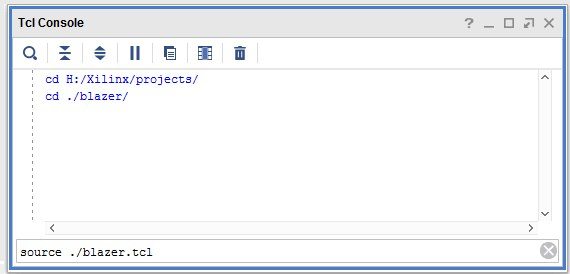
\includegraphics[scale=0.5]{source_project.jpg}
  \captionof{figure}{Развёртывание проекта в среде Vivado}
  \label{fig:bootstrap:configuration:source}
\end{center}

При использовании иной отладочной платы или камеры необходимо изменить отображение внутренней
логики на выводы микросхемы. Перепланировка выводов микросхемы осуществляется либо в специальном
разделе \en{I/O Planning} в разделе меню \en{Tools}, либо задать соотвествие в \en{constraints}
файле проекта. Дерево выбора \en{constraints} файла представлено на рисунке~\ref{fig:bootstrap:configuration:constraints_tree}

\begin{center}
  \centering
  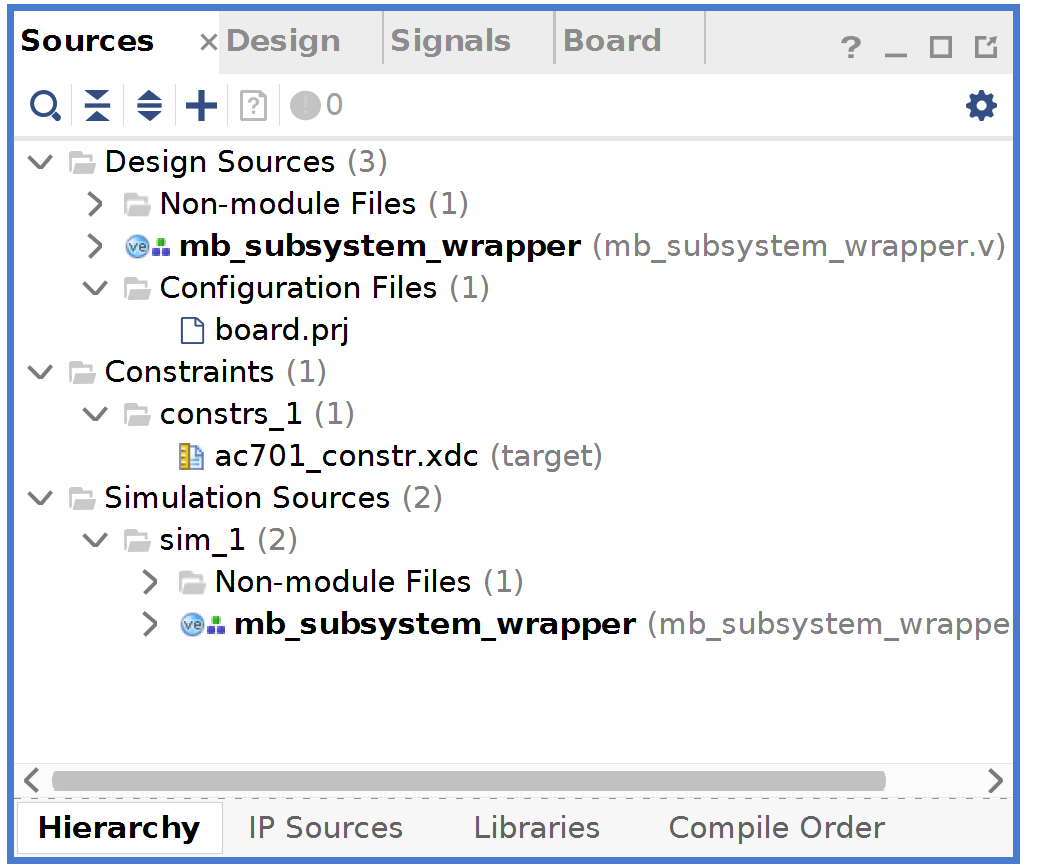
\includegraphics[scale=0.3]{constraints_tree.png}
  \captionof{figure}{Дерево исходного кода проекта}
  \label{fig:bootstrap:configuration:constraints_tree}
\end{center}

Пример \en{constraints} файла приведён на рисунке~\ref{fig:bootstrap:configuration:constraints_file}

\begin{center}
  \centering
  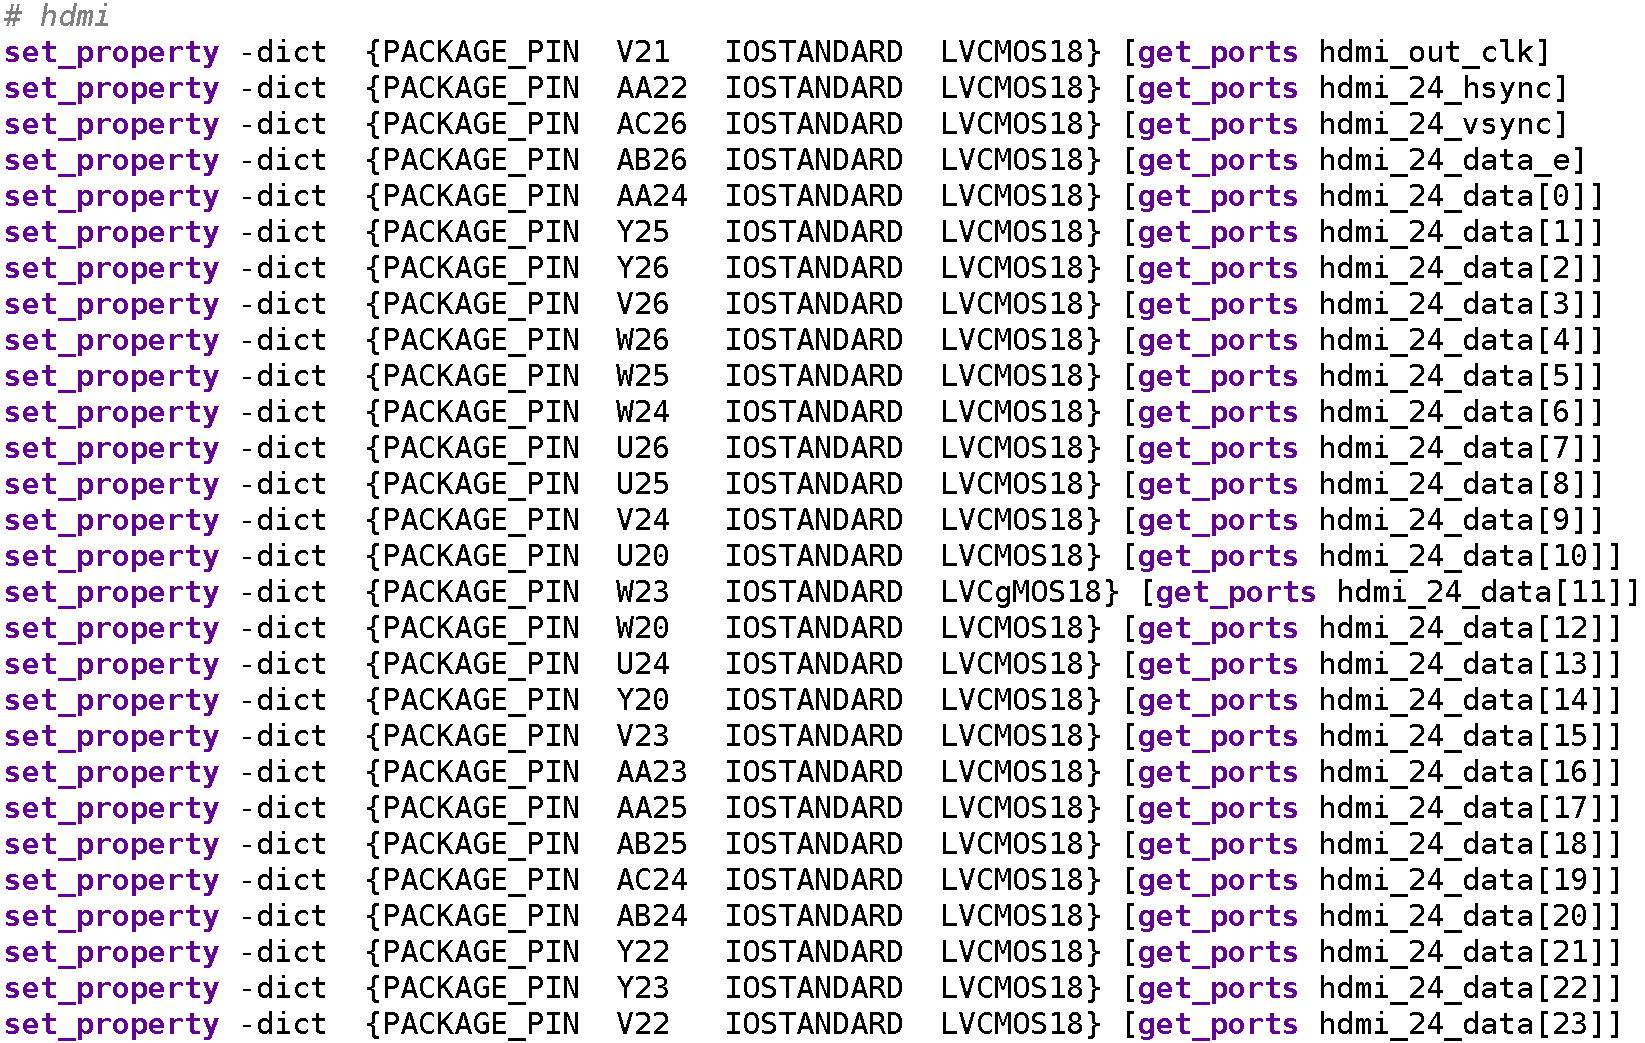
\includegraphics[scale=0.25]{constraints.png}
  \captionof{figure}{Пример \en{constraints} файла}
  \label{fig:bootstrap:configuration:constraints_file}
\end{center}

\en{Constraints} файл содержит соответствие внешних сигналов верхнего HDL модуля и
выводов микросхемы FPGA. Каждый вывод обладает уровнями допустимых напряжений, на что
следует обратить особое внимание при подключении периферии с нестандартными для FPGA
порогами. При этом только некоторые выводы могут передавать высокочастотные
тактовые сигналы, поэтому для выделения списка кандидатов на подключение из всего
множества выводов следует обратиться к технической документации микросхемы либо
предоставить выбор полуавтоматическому планировщику, работа которого должна сопровождаться
помощью со стороны пользователя.

Все необходимые изменения внешних сигналов системы могут производиться как в \en{block design},
так и в верхнем HDL модуле. При внесении изменений требуется перегенерировать модуль. Для
этого требуется открыть диалоговое меню при клике на файл на вершине иерархии, после чего выбрать пункт
\en{Create HDL Wrapper} и выбрать автоматическое обновление при изменении схемы проекта. Пример создания
верхнего модуля HDL приведено на рисунке~\ref{fig:bootstrap:configuration:hdl_wrapper}

\begin{center}
  \centering
  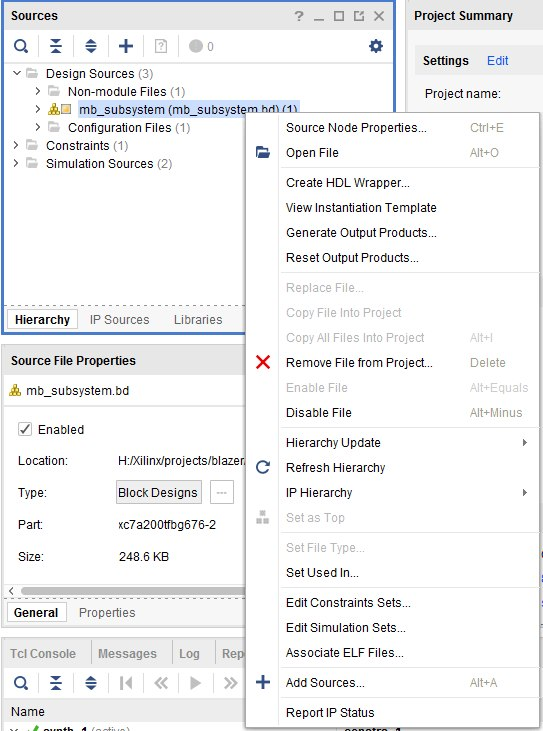
\includegraphics[scale=0.4]{hdl_wrapper.jpg}
  \captionof{figure}{Создание верхнего модуля HDL}
  \label{fig:bootstrap:configuration:hdl_wrapper}
\end{center}

После внесения изменений в проект следует этап синтезирования, реализации
синтезированного устройства на блоках микросхемы и генерация битстрима.

\subsection{Сборка проекта}
\label{sec:bootstrap:compilation}

Сборка проекта делится на несколько этапов, каждый из которых зависит от успешного
результата предыдущего.

На этапе синтеза HDL код переводится на уровень RTL (\en{Register Transfer Level}).
При наличии несинтезируемых конструкций в коде синтез прерывается с ошибкой. На этапе
синтеза присутствует возможность перезадать \en{constraints}, сменить метод синтеза и
просмотреть синтезированную схему. Пример синтезированной схемы представлен
на рисунке~\ref{fig:bootstrap:compilation:synthesis_result}

\begin{center}
  \centering
  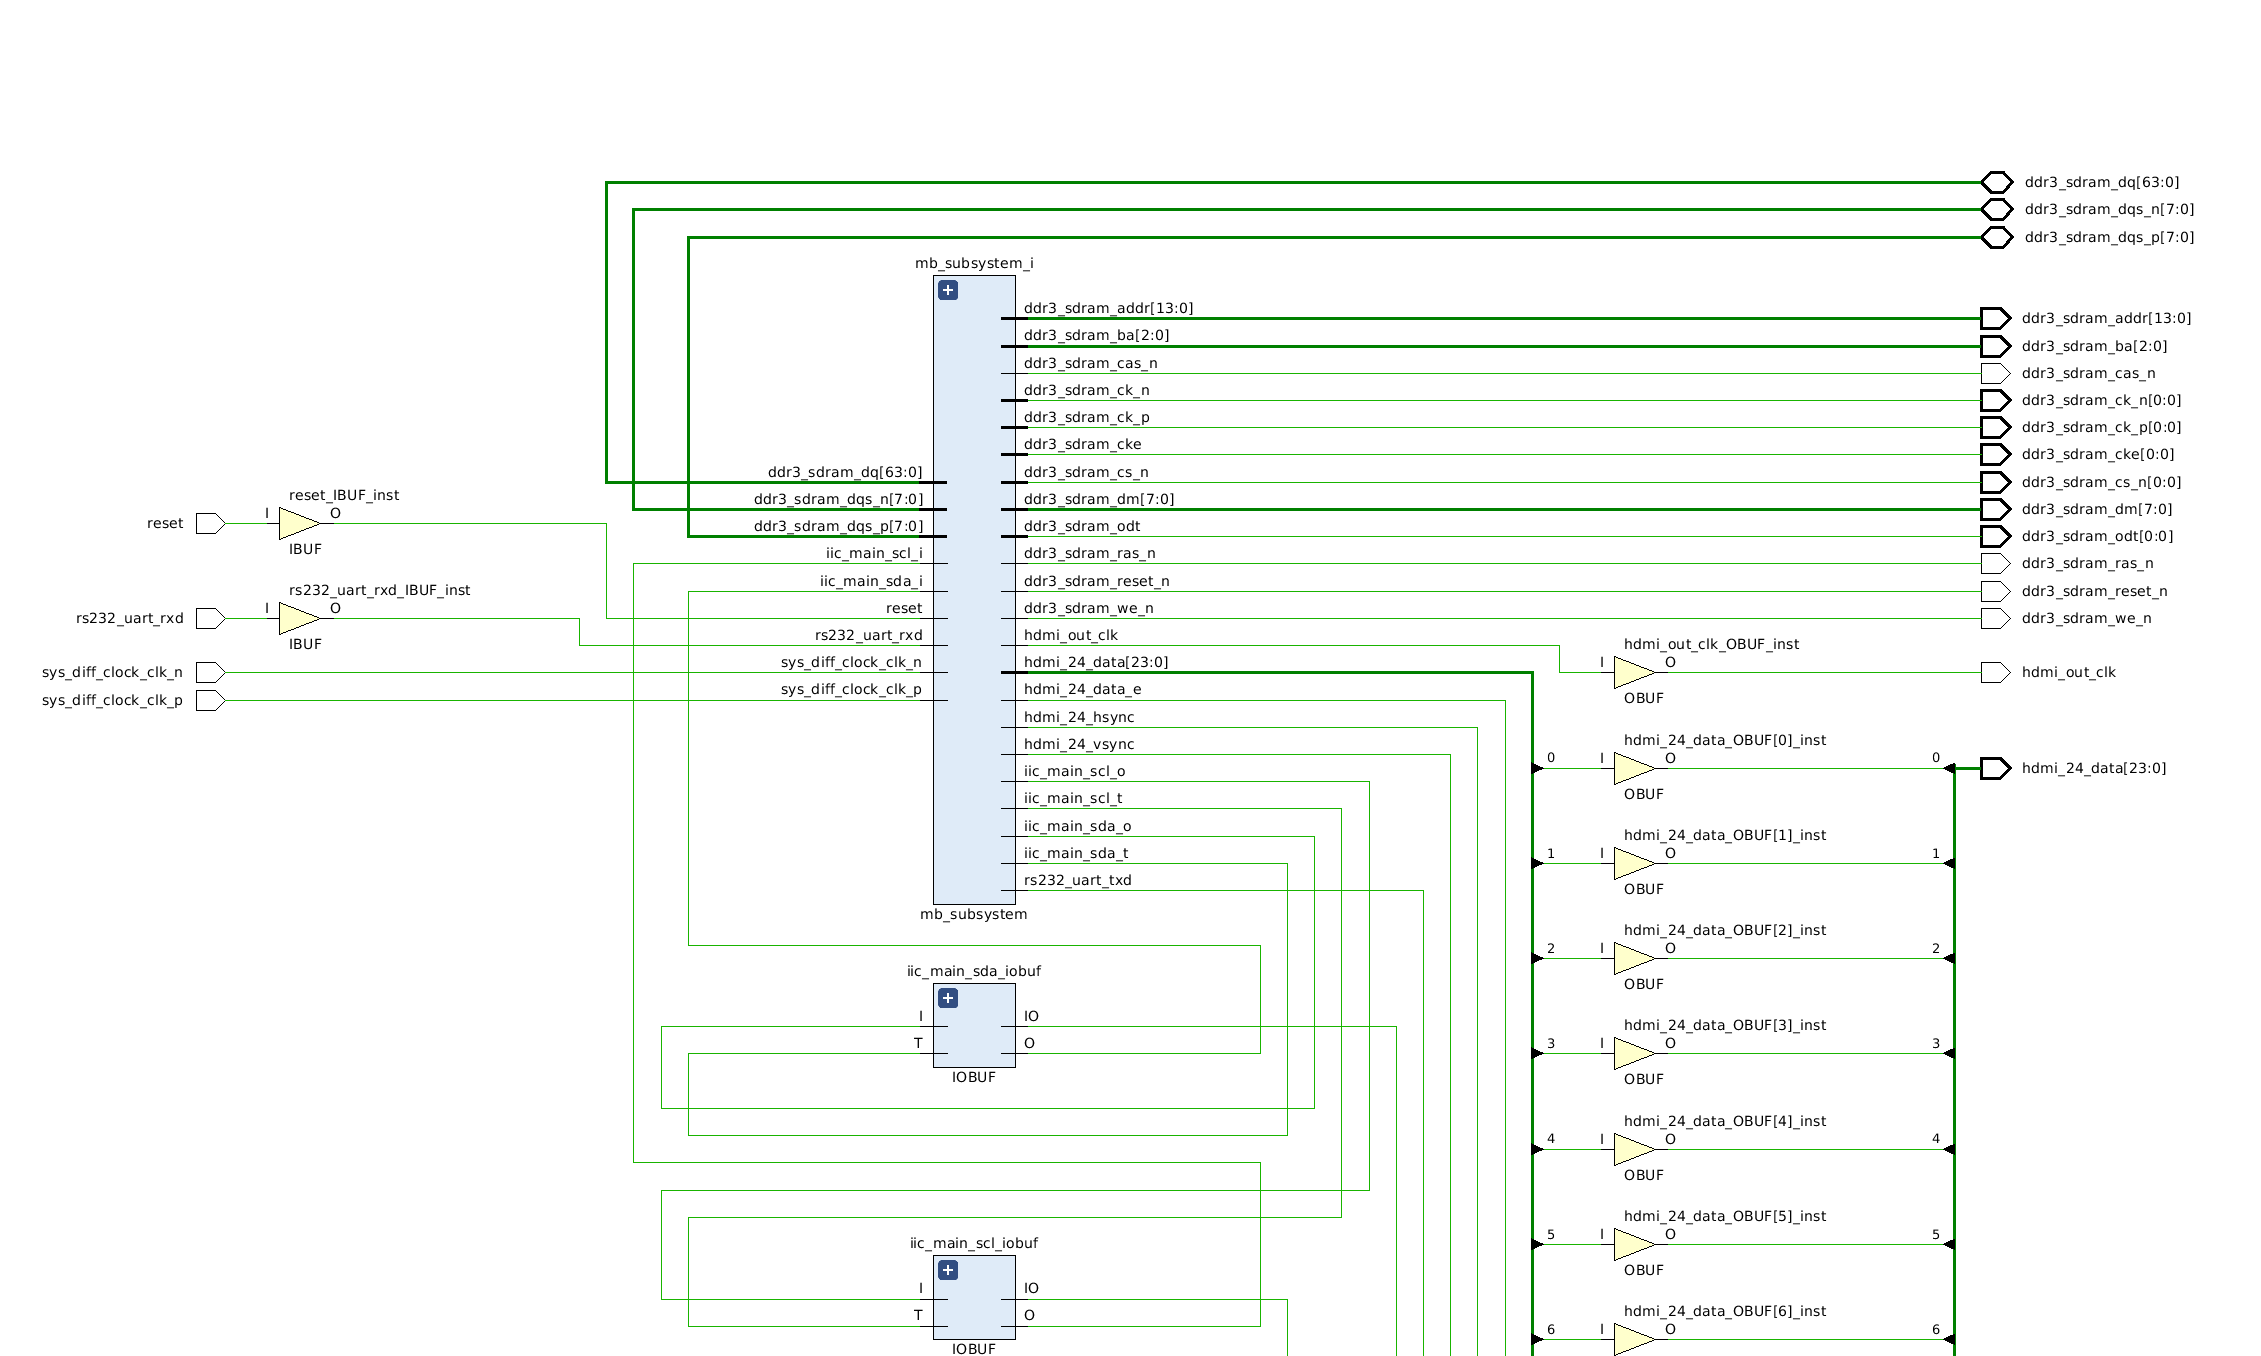
\includegraphics[scale=0.2]{synthesis_result.png}
  \captionof{figure}{Пример синтезированной схемы}
  \label{fig:bootstrap:compilation:synthesis_result}
\end{center}

Запуск синтеза производится соответствующим пунктом \en{Flow Navigator}. Блок работы с
синтезом представлен на рисунке~\ref{fig:bootstrap:compilation:synthesis_menu}

\begin{center}
  \centering
  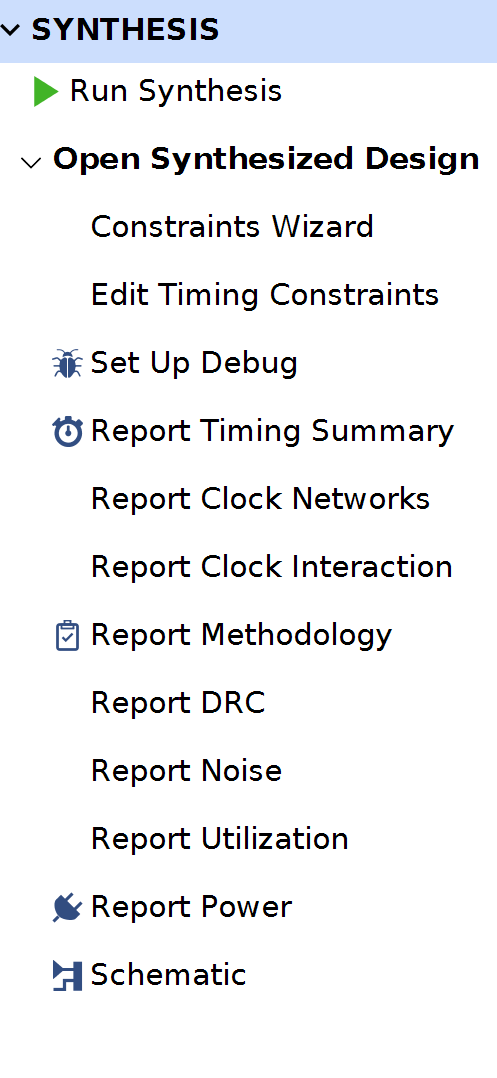
\includegraphics[scale=0.2]{synthesis_menu.png}
  \captionof{figure}{Блок работы с синтезом}
  \label{fig:bootstrap:compilation:synthesis_menu}
\end{center}

На этапе имплементации происходит реализация синтезированной схемы на логических блоках FPGA.
При этом каждому синтезированному блоку назначается КЛБ микросхемы, после назначения происходит
проводка маршрутов по трассам межсоединений. Алгоритмы имплементации занимаются поиском первого
подходящего по ограничения результата, а не лучшего среди нескольких кандидатов. Поэтому доведение
имплементации происходит путём модификации ограничений, подгоняя ограничения под различные случаи.

Пример реализации системы на ресурсах микросхемы
представлен на рисунке~\ref{fig:bootstrap:compilation:implementation_result}

\begin{center}
  \centering
  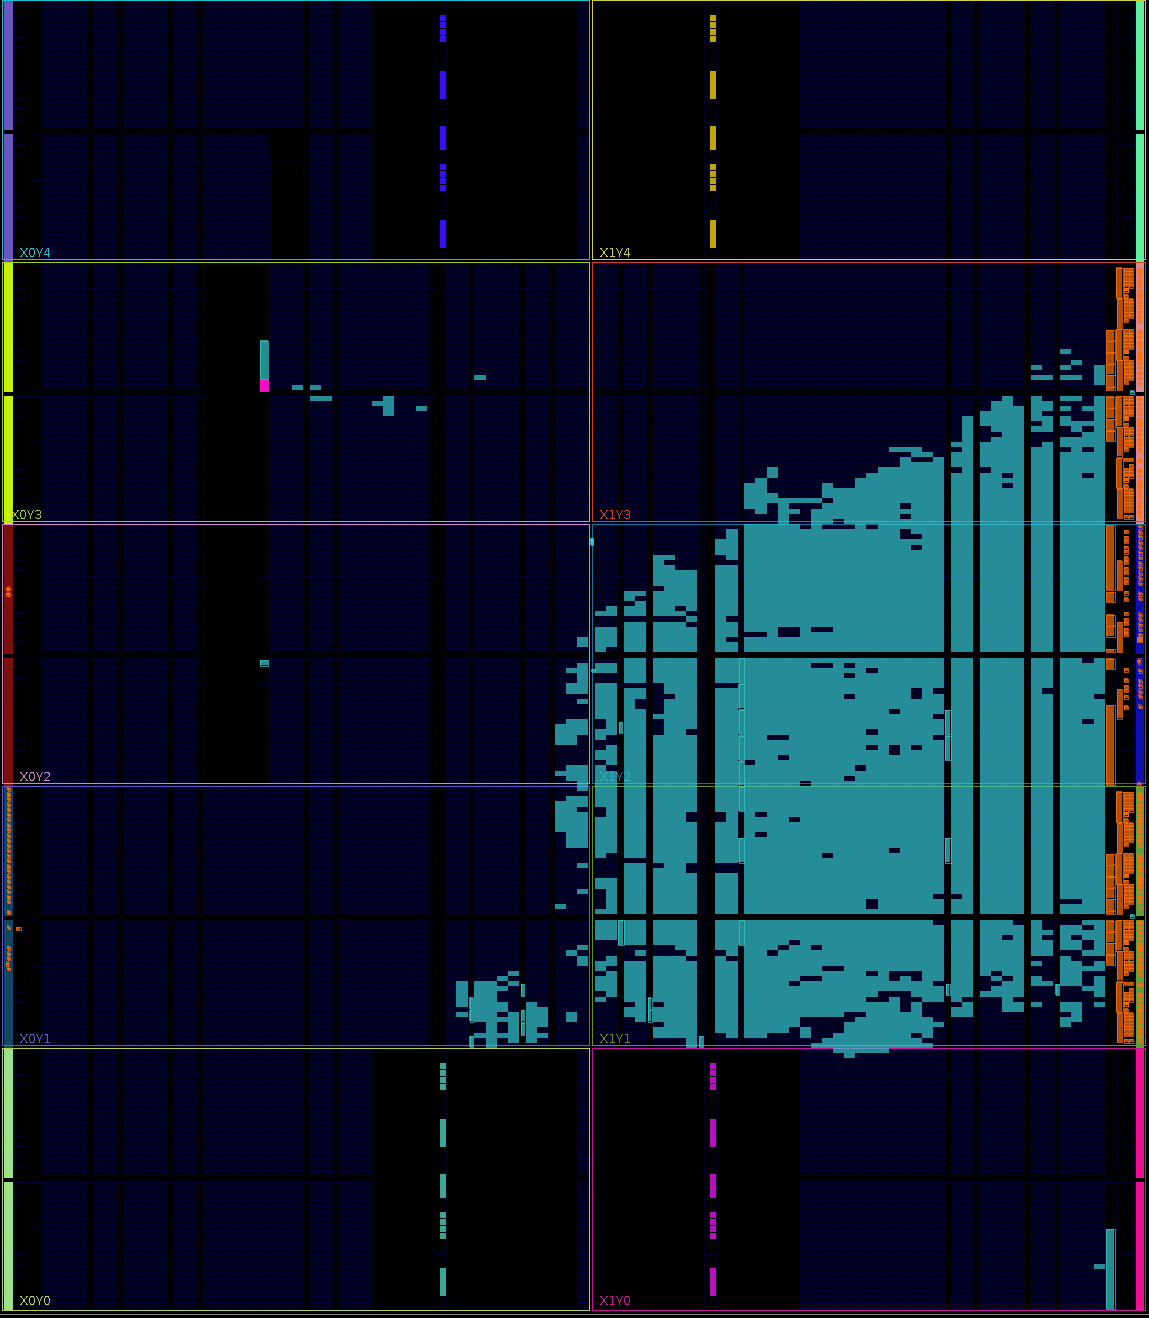
\includegraphics[scale=0.15]{implementation_result.png}
  \captionof{figure}{Результат имплементации системы}
  \label{fig:bootstrap:compilation:implementation_result}
\end{center}

Задать соответствие выводов микросхемы и выходов имплементированной схемы можно во вкладке \en{I/O Planning},
при этом стоит учесть описание назначения каждого вывода. Пример планировки выводов микросхемы
приведён на рисунке~\ref{fig:bootstrap:compilation:io_planning}

\begin{center}
  \centering
  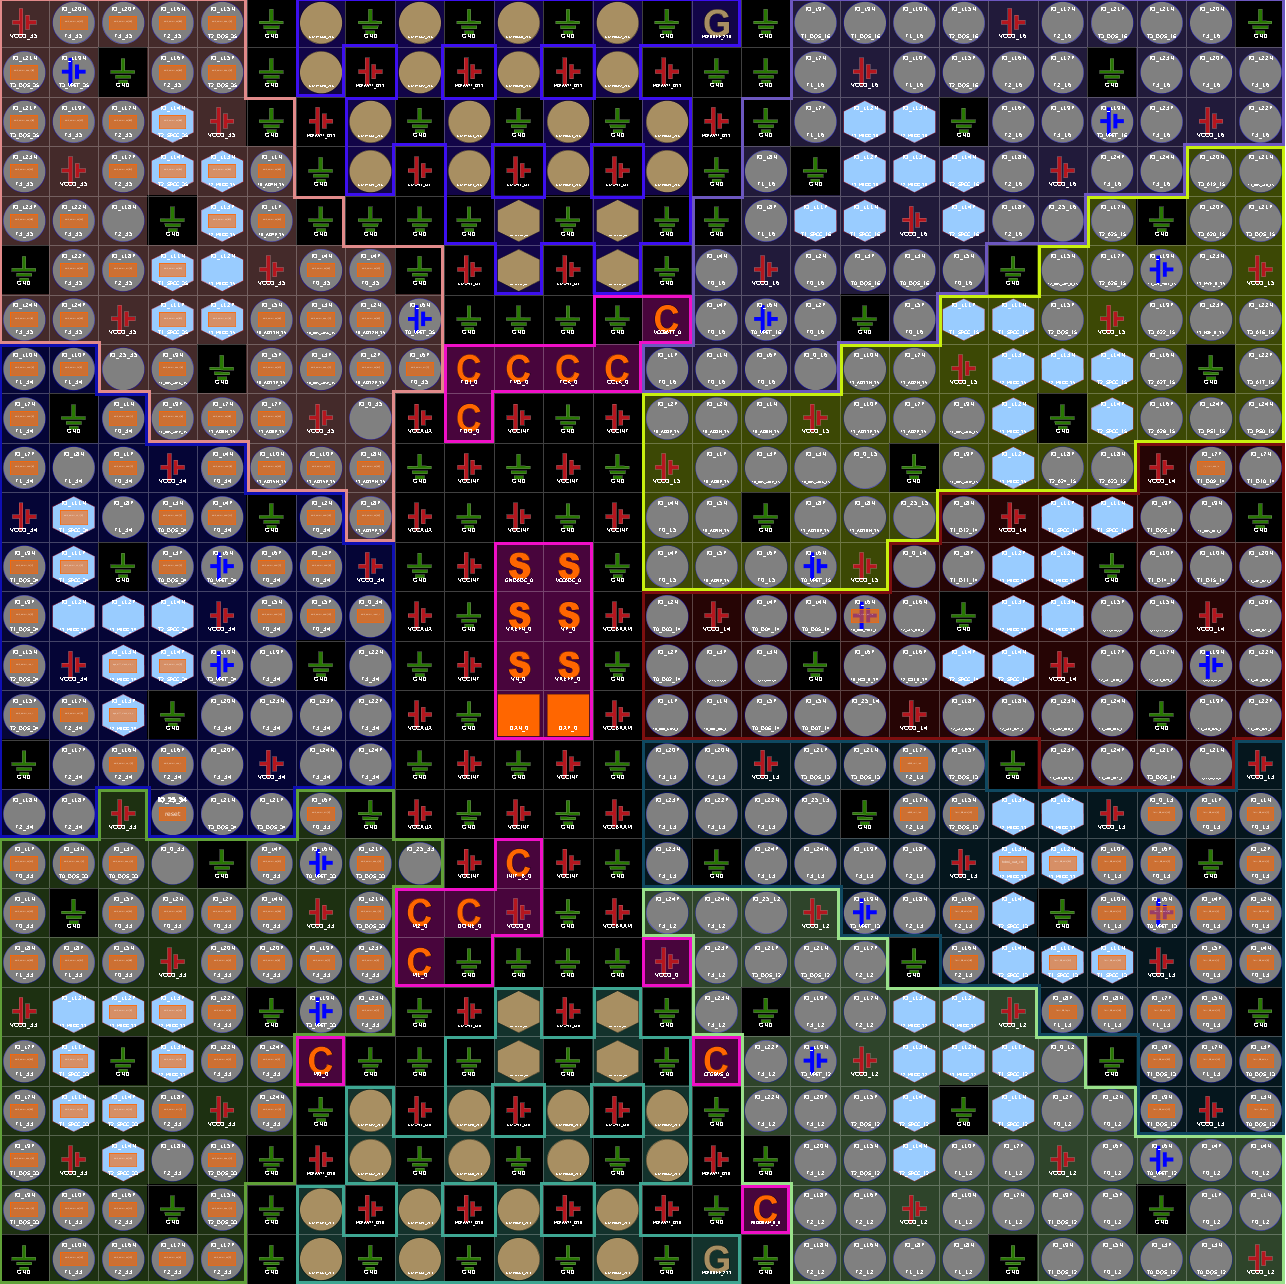
\includegraphics[scale=0.17]{io_planning.png}
  \captionof{figure}{Планировка назначения выводов микросхемы}
  \label{fig:bootstrap:compilation:io_planning}
\end{center}

Для запуска результата имплементации на микросхеме необходимо сгенерировать бистрим ---
поток битов, описывающих функциональное назначение блоков микросхемы и взаимосвязь
между ними. Процесс генерации битстрима схож с запуском синтеза.

\subsection{Запуск на отладочной плате}
\label{sec:bootstrap:board}

Далее будет описываться последовательность действий для отладочной платы
AC701. Для подготовки платы требуется выполнить следующие действия:
\begin{itemize}
  \item включить блок питания в сеть и подключить разъём к плате;
  \item подключить \en{Micro-USB} к соответствующему разъёму;
  \item подключить \en{Mini-USB} к конвертеру \en{USB to JTAG};
  \item перевести движковый переключатель питания в положение \en{On}.
\end{itemize}

После загорания на плате индикаторных светодиодов необходимо загрузить
битстрим и экспортировать аппаратную конфигурацию для последующего
применения в SDK.

Для загрузки битстрима необходимо нажать кнопку \en{Open Target},
после чего выбрать отладочную плату и начать загрузку. Экспорт
аппаратной конфигурации осуществляется в меню \en{File:Export:Export Hardware},
с выставленной опцией \en{Include Bitstream}.

После экспортирования конфигурации требуется запустить SDK из меню \en{File}.
Импорт проекта осуществляется в окне \en{Open Projects from File System} в меню \en{File}.
После успешного импорта проекта необходимо нажать пункт \en{Run Configurations} и
указать настройки согласно рисунку~\ref{fig:bootstrap:compilation:run_configuration}

\begin{center}
  \centering
  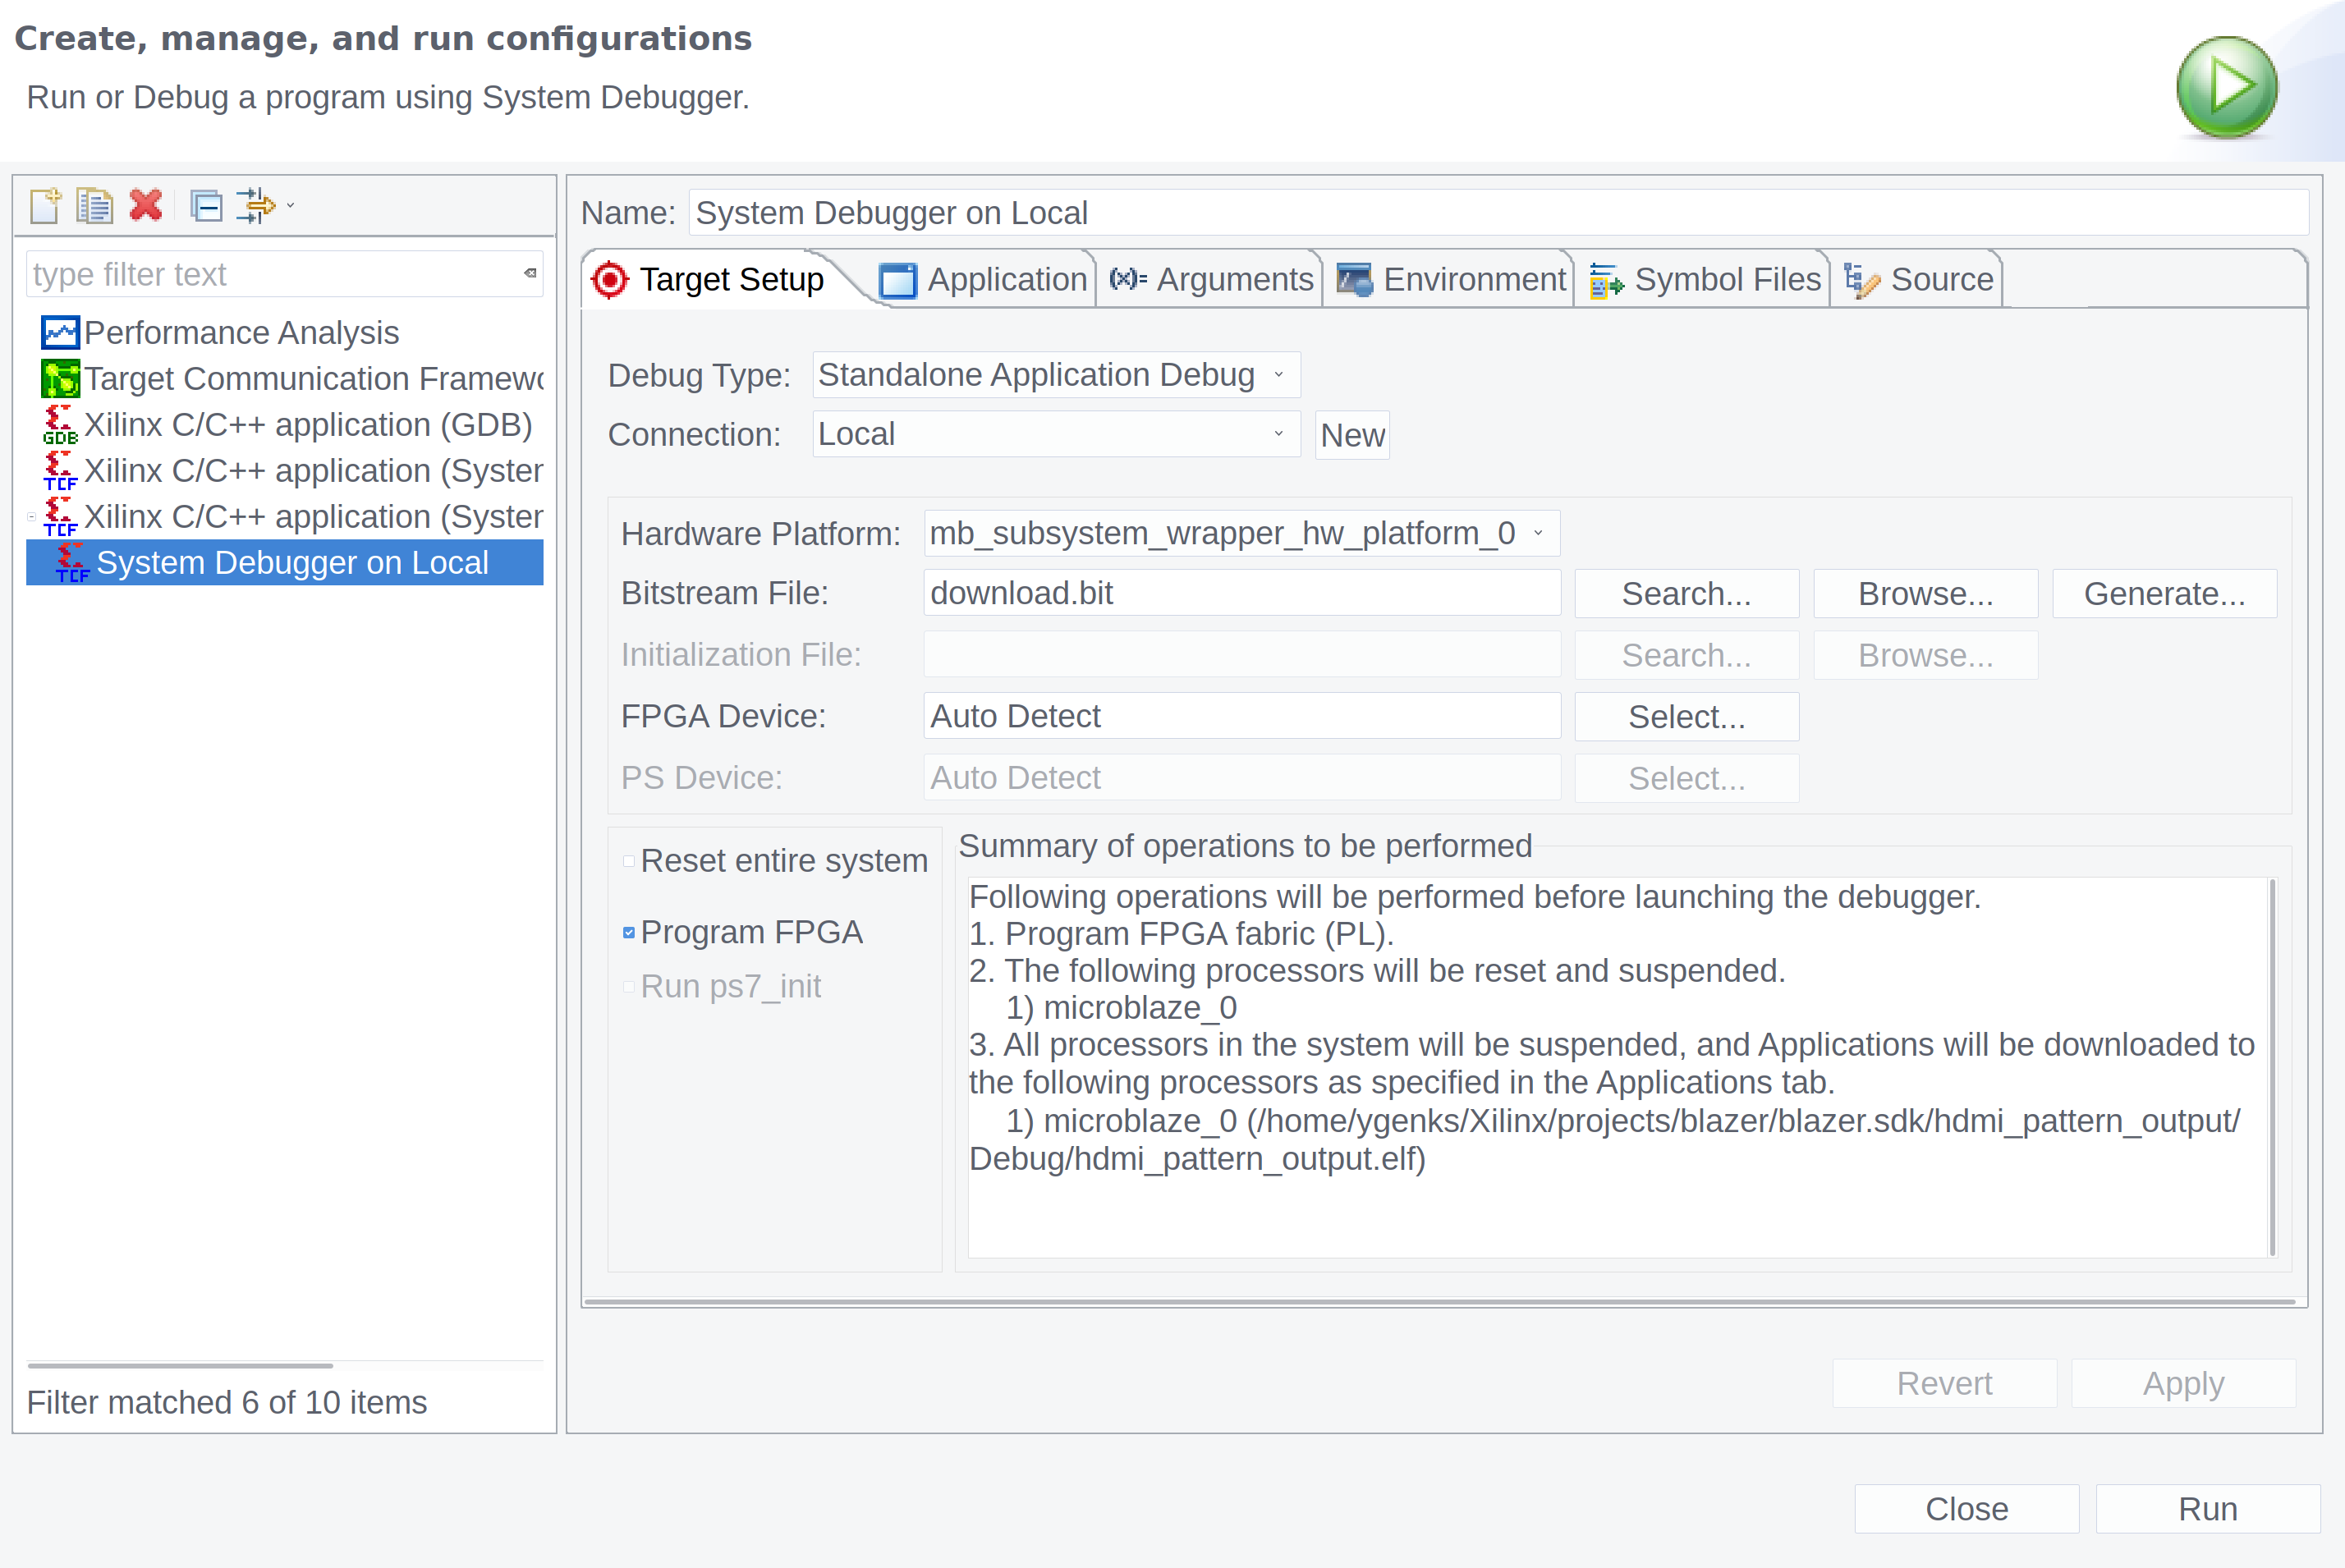
\includegraphics[scale=0.12]{run_configuration.png}
  \captionof{figure}{Конфигурация запуска}
  \label{fig:bootstrap:compilation:run_configuration}
\end{center}

После указания настроек для конфигурации запуска требуется нажать кнопку \en{Program FPGA},
указать настройки согласно рисунку~\ref{fig:bootstrap:compilation:program_fpga} и нажать
\en{Program}.

\begin{center}
  \centering
  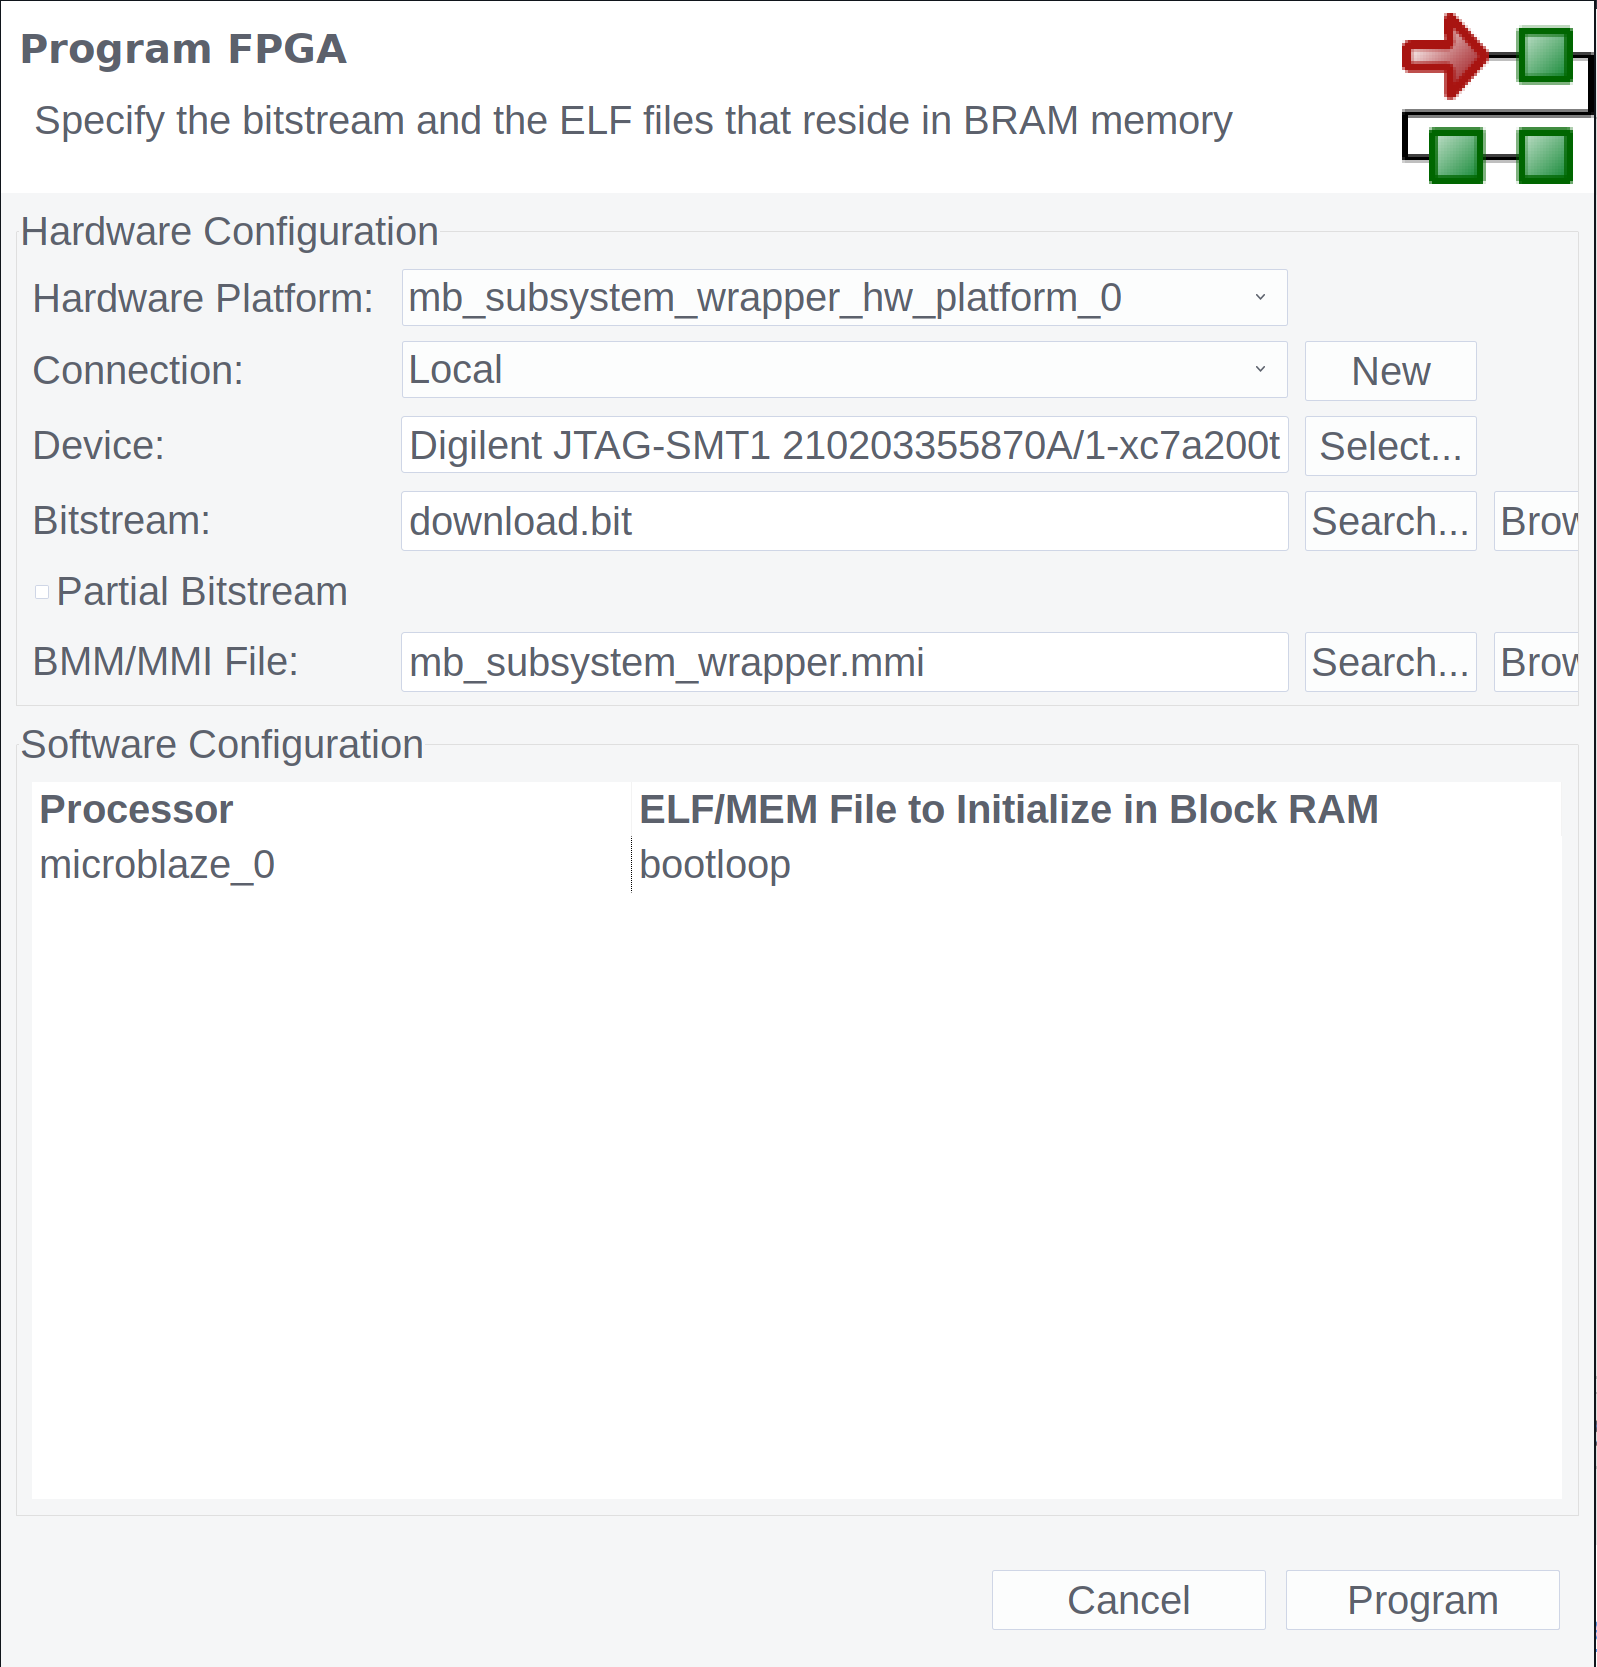
\includegraphics[scale=0.18]{program_fpga.png}
  \captionof{figure}{Загрузка битстрима в FPGA}
  \label{fig:bootstrap:compilation:program_fpga}
\end{center}

Для запуска проекта, в случае успешной загрузки битстрима, требуется нажать кнопку \en{Run} и
дождаться окончания сборки.


% \include{sec_ot}

\newdimen\origiwstr
\origiwstr=\fontdimen3\font
\fontdimen3\font=2\origiwstr
\section{ТЕХНИКО-ЭКОНОМИЧЕСКОЕ ОБОСНОВАНИЕ РАЗРАБОТКИ АППАРАТНОЙ СИСТЕМЫ ОБРАБОТКИ ВИДЕОПОТОКА}
\fontdimen3\font=\origiwstr
\label{sec:economics}


% \FPeval{\totalProgramSize}{15680}
% \FPeval{\totalProgramSizeCorrected}{8650}

% \FPeval{\normativeManDays}{224}

% \FPeval{\additionalComplexity}{0.12}
% \FPeval{\complexityFactor}{clip(1 + \additionalComplexity)}

% \FPeval{\stdModuleUsageFactor}{0.7}
% \FPeval{\originalityFactor}{0.7}

% \FPeval{\adjustedManDaysExact}{clip( \normativeManDays * \complexityFactor * \stdModuleUsageFactor * \originalityFactor )}
% \FPround{\adjustedManDays}{\adjustedManDaysExact}{0}

% \FPeval{\daysInYear}{365}
% \FPeval{\redLettersDaysInYear}{9}
% \FPeval{\weekendDaysInYear}{104}
% \FPeval{\vocationDaysInYear}{21}
% \FPeval{\workingDaysInYear}{ clip( \daysInYear - \redLettersDaysInYear - \weekendDaysInYear - \vocationDaysInYear ) }

% \FPeval{\developmentTimeMonths}{3}
% \FPeval{\developmentTimeYearsExact}{clip(\developmentTimeMonths / 12)}
% \FPround{\developmentTimeYears}{\developmentTimeYearsExact}{2}
% \FPeval{\requiredNumberOfProgrammersExact}{ clip( \adjustedManDays / (\developmentTimeYears * \workingDaysInYear) + 0.5 ) }

% % тут должно получаться 2 ))
% \FPtrunc{\requiredNumberOfProgrammers}{\requiredNumberOfProgrammersExact}{0}

% \FPeval{\tariffRateFirst}{600000}
% \FPeval{\tariffFactorFst}{3.04}
% \FPeval{\tariffFactorSnd}{3.48}


% \FPeval{\employmentFstExact}{clip( \adjustedManDays / \requiredNumberOfProgrammers )}
% \FPtrunc{\employmentFst}{\employmentFstExact}{0}

% \FPeval{\employmentSnd}{clip(\adjustedManDays - \employmentFst)}


% \FPeval{\workingHoursInMonth}{160}
% \FPeval{\salaryPerHourFstExact}{clip( \tariffRateFirst * \tariffFactorFst / \workingHoursInMonth )}
% \FPeval{\salaryPerHourSndExact}{clip( \tariffRateFirst * \tariffFactorSnd / \workingHoursInMonth )}
% \FPround{\salaryPerHourFst}{\salaryPerHourFstExact}{0}
% \FPround{\salaryPerHourSnd}{\salaryPerHourSndExact}{0}

% \FPeval{\bonusRate}{1.5}
% \FPeval{\workingHoursInDay}{8}
% \FPeval{\totalSalaryExact}{clip( \workingHoursInDay * \bonusRate * ( \salaryPerHourFst * \employmentFst + \salaryPerHourSnd * \employmentSnd ) )}
% \FPround{\totalSalary}{\totalSalaryExact}{0}

% \FPeval{\additionalSalaryNormative}{20}

% \FPeval{\additionalSalaryExact}{clip( \totalSalary * \additionalSalaryNormative / 100 )}
% \FPround{\additionalSalary}{\additionalSalaryExact}{0}

% \FPeval{\socialNeedsNormative}{0.5}
% \FPeval{\socialProtectionNormative}{34}
% \FPeval{\socialProtectionFund}{ clip(\socialNeedsNormative + \socialProtectionNormative) }

% \FPeval{\socialProtectionCostExact}{clip( (\totalSalary + \additionalSalary) * \socialProtectionFund / 100 )}
% \FPround{\socialProtectionCost}{\socialProtectionCostExact}{0}

% \FPeval{\taxWorkProtNormative}{4}
% \FPeval{\taxWorkProtCostExact}{clip( (\totalSalary + \additionalSalary) * \taxWorkProtNormative / 100 )}
% \FPround{\taxWorkProtCost}{\taxWorkProtCostExact}{0}
% \FPeval{\taxWorkProtCost}{0} % это считать не нужно, зануляем чтобы не менять формулы

% \FPeval{\stuffNormative}{3}
% \FPeval{\stuffCostExact}{clip( \totalSalary * \stuffNormative / 100 )}
% \FPeval{\stuffCost}{\stuffCostExact}

% \FPeval{\timeToDebugCodeNormative}{15}
% \FPeval{\reducingTimeToDebugFactor}{0.3}
% \FPeval{\adjustedTimeToDebugCodeNormative}{ clip( \timeToDebugCodeNormative * \reducingTimeToDebugFactor ) }

% \FPeval{\oneHourMachineTimeCost}{5000}

% \FPeval{\machineTimeCostExact}{ clip( \oneHourMachineTimeCost * \totalProgramSizeCorrected / 100 * \adjustedTimeToDebugCodeNormative ) }
% \FPround{\machineTimeCost}{\machineTimeCostExact}{0}

% \FPeval{\businessTripNormative}{15}
% \FPeval{\businessTripCostExact}{ clip( \totalSalary * \businessTripNormative / 100 ) }
% \FPround{\businessTripCost}{\businessTripCostExact}{0}

% \FPeval{\otherCostNormative}{20}
% \FPeval{\otherCostExact}{clip( \totalSalary * \otherCostNormative / 100 )}
% \FPround{\otherCost}{\otherCostExact}{0}

% \FPeval{\overheadCostNormative}{100}
% \FPeval{\overallCostExact}{clip( \totalSalary * \overheadCostNormative / 100 )}
% \FPround{\overheadCost}{\overallCostExact}{0}

% \FPeval{\overallCost}{clip( \totalSalary + \additionalSalary + \socialProtectionCost + \taxWorkProtCost + \stuffCost + \machineTimeCost + \businessTripCost + \otherCost + \overheadCost ) }

% \FPeval{\supportNormative}{30}
% \FPeval{\softwareSupportCostExact}{clip( \overallCost * \supportNormative / 100 )}
% \FPround{\softwareSupportCost}{\softwareSupportCostExact}{0}


% \FPeval{\baseCost}{ clip( \overallCost + \softwareSupportCost ) }

% \FPeval{\profitability}{35}
% \FPeval{\incomeExact}{clip( \baseCost / 100 * \profitability )}
% \FPround{\income}{\incomeExact}{0}

% \FPeval{\estimatedPrice}{clip( \income + \baseCost )}

% \FPeval{\localRepubTaxNormative}{3.9}
% \FPeval{\localRepubTaxExact}{clip( \estimatedPrice * \localRepubTaxNormative / (100 - \localRepubTaxNormative) )}
% \FPround{\localRepubTax}{\localRepubTaxExact}{0}
% \FPeval{\localRepubTax}{0}

% \FPeval{\ndsNormative}{20}
% \FPeval{\ndsExact}{clip( (\estimatedPrice + \localRepubTax) / 100 * \ndsNormative )}
% \FPround{\nds}{\ndsExact}{0}


% \FPeval{\sellingPrice}{clip( \estimatedPrice + \localRepubTax + \nds )}

% \FPeval{\taxForIncome}{18}
% \FPeval{\incomeWithTaxes}{clip(\income * (1 - \taxForIncome / 100))}
% \FPround\incomeWithTaxes{\incomeWithTaxes}{0}

%%%%%%%%%%%%%%%%%%%%%%%%%%%%%%%%%%%%%%%%%%%%%%%%%%

\subsection{Характеристика аппаратной системы обработки видеопотока}
\label{sec:economics:characteristics}

Обработка видеопотока --- сложная в техническом плане задача. Её решение сопровождается
применением широкого спектра инженерных средств. Изменчивость параметров видео во
времени не позволяют конструировать узкоспециализированные устройства или программы по его
обработке, поэтому часто применяется системный подход.

Достоинствами рассматриваемой системы являются модульность и гибкость, возможность
смены алгоритмов обработки изображений во время работы системы, поддержка работы в приложениях,
требующих предсказуемого времени работы его компонентов, а также обладает возможностью
обрабатывать видео выского разрешения (HDTV и выше).

Применение данной системы позвляет рационализировать затраты на оборудования для обработки видео,
позволяя потребителю дополнять существующий конвейер своими блоками обработки, не приобретая
для каждой новой операции отдельное устройство. В случае работы системы в встраиваемом виде
минизирует энергопотребление конечного продукта и его размеры, сохраняя при этом высокую скорость работы.

Система рассчитана на применение в различных отраслях, но особенно хорошо проявляет себя в машиностроении,
авиастроении, космической промышленности и разработке \en{embedded} устройств.

\subsection{Расчёт стоимостной оценки затрат}
\label{sec:economics:cost_estimation}

\subsubsection{Расчёт затрат на разработку аппаратной части}
\label{sec:economics:cost_estimation:hardware}

Расчёт затрат на зарботную плату разработчиков аппаратной части представлен в таблице~\ref{table:economics:cost_estimation:hardware:employee}

\begin{table}[ht]
  \caption{Расчёт основной зарботной платы исполнителей}
  \label{table:economics:cost_estimation:hardware:employee}
  \begin{tabular}{| >{\centering}m{0.4\textwidth}
                  | >{\centering}m{0.18\textwidth}
                  | >{\centering}m{0.15\textwidth}
                  | >{\centering\arraybackslash}m{0.15\textwidth}|}
   \hline
    Категория исполнителя & Эффективный фонд времени работы, дн. & Дневная тарифная ставка, руб. & Тарифная заработная плата, руб. \\
   \hline
    Инженер-проекта & $ 20 $ & $ 80 $ & $ 1600 $ \\
   \hline
    Инженер-системотехник & $ 20 $ & $ 60 $ & $ 1200 $ \\
   \hline
    Всего & & & $ 2800 $ \\
   \hline
    Премия (50 \%) & & & $ 1400 $ \\
   \hline
    Основная заработная плата & & & $ 4200 $  \\
   \hline
  \end{tabular}
\end{table}

Расчёт затрат на разработку аппаратной части представлен в таблице~\ref{table:economics:cost_estimation:hardware:employee_total}

\begin{table}[ht]
  \caption{Расчёт затрат на разработку аппаратной части}
  \label{table:economics:cost_estimation:hardware:employee_total}
  \begin{tabular}{| >{\centering}m{0.3\textwidth}
                  | >{\centering}m{0.4\textwidth}
                  | >{\centering\arraybackslash}m{0.2\textwidth}|}
   \hline
    Наименование статьи затрат & Расчёт & Значение, руб. \\
   \hline
    Основная заработная плата разработчиков & См. таблицу~\ref{table:economics:cost_estimation:hardware:employee} & $ 4200 $ \\
   \hline
    Дополнительная зарплата & $ \dfrac{4200 \cdot 20}{100} $ & $ 840 $ \\
   \hline
    Отчисления на социальные нужды & $ \dfrac{(4200 + 840) \cdot 34,6}{100} $ & $ 1743 $ \\
   \hline
  \end{tabular}
\end{table}

Расчёт затрат на создание прототипа системы обработки видеопотока представлен в таблице~\ref{table:economics:cost_estimation:hardware:prerequisites}

\begin{table}[ht]
  \caption{Расчёт затрат на комплектующие и средства разработки}
  \label{table:economics:cost_estimation:hardware:prerequisites}
  \begin{tabular}{| >{\centering}m{0.3\textwidth}
                  | >{\centering}m{0.15\textwidth}
                  | >{\centering}m{0.15\textwidth}
                  | >{\centering}m{0.15\textwidth}
                  | >{\centering\arraybackslash}m{0.15\textwidth}|}
  \hline
    Наименование оборудования или ПО & Тип, марка & Количество, шт. & Цена за единицу, руб. & Стоимость, руб. \\
  \hline
    Xilinx Artix-7 FPGA Evaluation Kit & AC701 & $ 1 $ & $ 2619 $ & $ 2619 $ \\
  \hline
    Модуль камеры & MT9T031 & $ 1 $ & $ 43 $ & $ 43 $ \\
  \hline
    САПР Vivado Design Suite & HL Design Edition & $ 1 $ & $ 2023 $ & $ 2023 $ \\
  \hline
    Всего & &  &  & $ 4685 $ \\
  \hline
    Транспортно-заготовительные расходы для комплектующих (20 \%)  & & & & $ 937 $ \\
  \hline
    Всего с транспортно-заготовительными расходами & & & & $ 5622 $ \\
  \hline
  \end{tabular}
\end{table}

Данные затраты являются единовременными затратами на проектирование, в дальнейшем предприятие может использовать
спроектированную систему на базе любой микросхемы FPGA седьмой серии компании Xilinx. В данном случае
необходимо спроектировать минимальную схему, содержащую следующую периферию:

\begin{itemize}
  \item модуль КМОП или ПЗС матрицы с микроконтроллером;
  \item устройство вывода HDMI;
  \item I2C контроллер;
  \item DDR-память для хранения кадров поступающих из камеры;
\end{itemize}

\subsubsection{Расчёт затрат на разработку программной части}
\label{sec:economics:cost_estimation:software}

Разработка программной части включает в себя написание конфигурационного кода
для контроллеров HDMI, I2C и модуля камеры, проектирование API для
передачи кадров в оперативную память и последующую их передачу на HDMI-порт.

Расчёт затрат на зарботную плату разработчиков программной части представлен в таблице~\ref{table:economics:cost_estimation:software:employee}

\begin{table}[ht]
  \caption{Расчёт основной зарботной платы исполнителей}
  \label{table:economics:cost_estimation:software:employee}
  \begin{tabular}{| >{\centering}m{0.4\textwidth}
                  | >{\centering}m{0.18\textwidth}
                  | >{\centering}m{0.15\textwidth}
                  | >{\centering\arraybackslash}m{0.15\textwidth}|}
   \hline
    Категория исполнителя & Эффективный фонд времени работы, дн. & Дневная тарифная ставка, руб. & Тарифная заработная плата, руб. \\
   \hline
    Ведущий инженер-программист & $ 15 $ & $ 80 $ & $ 1200 $ \\
   \hline
    Инженер-программист 2.к & $ 15 $ & $ 60 $ & $ 900 $ \\
   \hline
    Всего & & & $ 2100 $ \\
   \hline
    Премия (50 \%) & & & $ 1050 $ \\
   \hline
    Основная заработная плата & & & $ 3150 $  \\
   \hline
  \end{tabular}
\end{table}

Расчёт затрат на разработку программной части представлен в таблице~\ref{table:economics:cost_estimation:software:employee_total}

\begin{table}[ht]
  \caption{Расчёт затрат на разработку программной части}
  \label{table:economics:cost_estimation:software:employee_total}
  \begin{tabular}{| >{\centering}m{0.3\textwidth}
                  | >{\centering}m{0.4\textwidth}
                  | >{\centering\arraybackslash}m{0.2\textwidth}|}
   \hline
    Наименование статьи затрат & Расчёт & Значение, руб. \\
   \hline
    Основная заработная плата разработчиков & См. таблицу~\ref{table:economics:cost_estimation:software:employee} & $ 3150 $ \\
   \hline
    Дополнительная зарплата & $ \dfrac{3150 \cdot 20}{100} $ & $ 630 $ \\
   \hline
    Отчисления на социальные нужды & $ \dfrac{(3150 + 630) \cdot 34,6}{100} $ & $ 1307 $ \\
   \hline
  \end{tabular}
\end{table}

\subsubsection{Расчёт капитальных вложений}
\label{sec:economics:capital_investment}

Капитальные вложения рассчитываются с учётом получения прибыли с продажи готовой системы,
а не минимально возможной платы, т.к. последнее потребует организации сложного производства.
Расчёт капитальных вложений проведён в соответствии с таблицей~\ref{table:economics:capital_investment_total}

\begin{table}[ht!]
  \caption{Капитальные вложения на разработку системы}
  \label{table:economics:capital_investment_total}
  \begin{tabular}{| >{\centering}m{0.4\textwidth}
                  | >{\centering}m{0.3\textwidth}
                  | >{\centering\arraybackslash}m{0.2\textwidth}|}
   \hline
    Наименование затрат & Расчёт & Сумма, руб. \\
   \hline
    Затраты на разработку аппаратной части & Таблица~\ref{table:economics:cost_estimation:hardware:employee_total} & $ 6783 $ \\
   \hline
    Затраты на разработку программной части & Таблица~\ref{table:economics:cost_estimation:software:employee_total}  & $ 5087 $ \\
   \hline
    Затраты на комплектующие и средства разработки & Таблица~\ref{table:economics:cost_estimation:hardware:prerequisites}  & $ 5622 $ \\
   \hline
    Всего &  & $ 17492 $ \\
   \hline
    Накладные расходы (50 \%) & $ \dfrac{17492 \cdot 50}{100} $ & $ 8746 $ \\[1cm]
   \hline
    Всего затрат на разработку & $ 17492 + 8746 $ & $ 26238 $ \\
   \hline
    Прибыль (50 \%) & $ \dfrac{26238 \cdot 50}{100} $ & $ 13119 $ \\[1cm]
   \hline
    Отпускная цена & $ 26238 + 13119 $ & $ 39357 $ \\
   \hline
    Налог на добавленную стоимость (20 \%) & $ \dfrac{39357 \cdot 20}{100} $ & $ 7871,4 $ \\[1cm]
   \hline
    Отпускная цена с НДС & $ 39357 + 7871,4 $ & $ 47228,4 $ \\
   \hline
  \end{tabular}
\end{table}


\subsection{Расчёт экономической эффективности разработки системы обработки видеопотока}
\label{sec:economics:efficiency}

Экономическим эффектом у предприятия-разработчика системы является чистая прибыль, остающаяся в распоряжении организации, которая составит:

\begin{equation}
  \label{eq:economics:income}
  \text{П} = 13119 - \dfrac{13119 \cdot 18}{100} = \SI{10757,58}{\text{руб.}}
\end{equation}

Рентабельность затрат на разработку данной системы для организации-разработчика составит:

\begin{equation}
  \label{eq:economics:profit}
  \text{P} = \dfrac{10757,58}{26238} * 100\% = 41\% % какого хрена совпало с методой???
\end{equation}

На основании полученных результатов экономического обоснования можно сделать вывод,
что затраты на разработку и внедрение данной системы являются экономически эффективными
как для предприятия-разработчика, так и для предприятия-заказчика системы. После выполнения
работ предприятие-разработчик получает чистую прибыль в размере 10757,58 руб., при этом
рентабельность разработки и установки составит 41\%.


% \include{sec_final}

% Зачем: Изменение надписи для списка литературы
% Почему: Пункт 2.8.1 Требований по оформлению пояснительной записки.
\renewcommand{\bibsection}{\sectioncentered*{СПИСОК ИСПОЛЬЗОВАННЫХ ИСТОЧНИКОВ}}
\phantomsection\pagebreak% исправляет нумерацию в документе и исправляет гиперссылки в pdf
\addcontentsline{toc}{section}{СПИСОК ИСПОЛЬЗОВАННЫХ ИСТОЧНИКОВ}

% Зачем: Печать списка литературы. База данных литературы - файл bibliography_database.bib

\bibliography{bibliography_database}


\appendix
\addcontentsline{toc}{section}{ПРИЛОЖЕНИЕ А}
% \addtocounter{page}{1}
\newpage
\addcontentsline{toc}{section}{ПРИЛОЖЕНИЕ Б}
лолкек


% \includepdf позволяет включить в результирующий pdf документ часть другого pdf документа, сделанного
% например не с помощью TeX. Бывает полезно, если какие-то диаграммны нарисованы, например, с помощью 
% Microoft Office и сохранены в pdf.
%\includepdf[pages={-}]{documents_list.pdf}

\end{document}